\documentclass[a4paper,12pt]{report}
\usepackage{a4wide}

%\documentclass[a5paper,10pt]{book}
%\usepackage[top=23mm, bottom=18mm, left=15mm, right=25mm]{geometry}
%\geometry{papersize={170mm,220mm}}


\usepackage[utf8x]{inputenc}
\usepackage[danish]{babel}

\usepackage{xr-hyper} %Externe hyper-ref
\usepackage[colorlinks=true, hyperindex=true, linkcolor=minmblaa, citecolor=minmblaa, urlcolor=minmblaa]{hyperref}
\hypersetup{colorlinks=true,filecolor=minmblaa,bookmarksnumbered=true} %Til hyperreferencer. Referencer med farver
\usepackage{needspace} % giver mulighed for at kræve at der skal være et antal tomme linier på siden før ellers indsættes et sideskift.
\usepackage{framed} %Bokse
\usepackage{wrapfig}

\usepackage{amsmath,amsfonts,amssymb,amsthm,mathtools} %Matematikpakker

\setlength{\parindent}{0mm} %Ingen Indhak i første linje i afsnit

\usepackage{color} %Farvepakke

\usepackage{array}
\usepackage{colortbl}
\usepackage{multirow} %Til at flette rækker i tabeller.

\usepackage{verbatim,mhchem}



	% DOWNLOAD FRA: http://sarovar.org/frs/?group_id=52&release_id=97
	% Læg i directory for hoved TEX fil
%\usepackage[draft]{pdfdraftcopy}
%\draftstring{Licens: Kasper Langt Mellemnavn Skårhøj}
%\draftfontsize{30}
	%\draftfontfamily{hlh}
	%\draftangle{45}
	%\definecolor{mycolor}{rgb}{.825,.855,1}
	%\draftcolor{mycolor}
	%\draftfontattrib



% = Sidehoved =
\usepackage{fancyhdr}
\pagestyle{fancy}
\renewcommand{\sectionmark}[1]{\markright{\protect\titlegraphic{dturoed}\textcolor{dtugraa}{\thesection~\MakeUppercase{#1}}}} % \thesection.\
\fancyhead{}
\fancyfoot{}
\fancyhead[R]{\titlefont\thepage}
\fancyhead[C]{}
\fancyhead[L]{\titlefont \small eNote \MakeUppercase{~\thechapter}~\hspace*{1ex}\rightmark}
\renewcommand\headrulewidth{0pt}
\fancypagestyle{plain}{\fancyfoot[C]{}}% {\titlefont\footnotesize\thepage}}
\setlength{\headheight}{15pt}


% = Længder
%\newlength{\envtblsep}\setlength{\envtblsep}{1\FrameSep}
\newlength{\obsl}\setlength{\obsl}{\textwidth-1.2cm-13.2pt}

% Includes:

% =     Fonts (select one)    =
\usepackage{mathpazo}\linespread{1.05} % Palatino needs more leading (space between lines)
\usepackage{bm} % bold math, must be loaded after the fontpackages

% % Til overskrifter
\DeclareTextFontCommand{\th}{\fontencoding{T1}\fontfamily{phv}\fontseries{b}\selectfont}
\newcommand\titlefont{\fontencoding{T1}\fontfamily{phv}\selectfont}


% =     PGF grafik      =
\usepackage{tikz}
\newcommand\titlegraphic[1]{%
\tikz[baseline] %
\draw[thick,color=#1]
(0pt  ,-0.25em) -- (0pt  ,0.85em)
(2.5pt,-0.25em) -- (2.5pt,0.85em)
(5pt  ,-0.25em) -- (5pt  ,0.85em)
(7.5pt,-0.25em) -- (7.5pt,0.85em);\hspace*{0.8ex} %
}

\newcommand\titlegraphicwide[1]{%
\tikz[baseline] %
\draw[line width=0.8mm,color=#1]
(0pt  ,-0.25em) -- (0pt  ,0.85em)
(4.5pt,-0.25em) -- (4.5pt,0.85em)
(9pt  ,-0.25em) -- (9pt  ,0.85em)
(13.5pt,-0.25em) -- (13.5pt,0.85em);\hspace*{0.8ex} %
}


% =      Title Layout      =
\usepackage{titlesec}
\makeatletter
\titleformat{\chapter}
	[display] % Shape
	{\titlefont\Huge\flushleft} % Title and label format
	{\titlefont\LARGE\bfseries \titlegraphicwide{dturoed}\textcolor{dtugraa}{\@chapapp~\thechapter}} % label
	{0.9em} % label/title separation
	{} % before code
	[] % after code
\makeatother
\titleformat{\section}
	[hang] % Shape
	{\titlefont\Large\flushleft} % Title and label format
	{\thesection} % label
	{0.9em} % label/title separation
	{} % before code
	[] % after code
\titleformat{\subsection}
	[hang] % Shape
	{\titlefont\large} % Title and label format
	{\thesubsection} % label
	{0.9em} % label/title separation
	{} % before code
	[] % after code
\titlespacing{\subsection}{0pt}{*6}{*1.5}
\titleformat{\subsubsection}
	[hang] % Shape
	{\titlefont} % Title and label format
	{\thesubsubsection} % label
	{0.9em} % label/title separation
	{} % before code
	[] % after code



% = Farver
\definecolor{dturoed}{rgb}{0.6, 0.0, 0.0}
\definecolor{dtugraa}{rgb}{0.5, 0.5, 0.5}	% Lidt mørkere. Korrekt = 0.4
\definecolor{mingroenstreg}{rgb}{0.4,0.8,0}	% Sekundærfarve 14 : 102/204/0	(Forårsgrøn) -> Eksempler
\definecolor{mingroen}{rgb}{0.32,0.64,0}		% Sekundærfarve 14, 80% mørkere (tekst)
\definecolor{minorangestreg}{rgb}{1,0.6,0}		% Sekundærfarve 1 : 255/153/0	(Orange) -> Opgaver
\definecolor{minorange}{rgb}{0.8,0.48,0}		% Sekundærfarve 1 , 80% mørkere (tekst)

\definecolor{minblaa}{rgb}{0.2,0.4,0.8}	% Sekundærfarve 13 , 51/102/204 	( Blå -> Definitioner etc)
\definecolor{minmblaa}{rgb}{0.16,0.32,0.64}	% Sekundærfarve 13 , 80% mørkere (tekst)
\definecolor{thmbackground}{rgb}{0.97,.97, 0.99}	% Farve 13 - lys baggrund

\definecolor{mingraastreg}{rgb}{.5,.5,.5}
\definecolor{hvadbackground}{rgb}{0.97,.97, 0.97}
\definecolor{sumgul}{rgb}{1,1,.8}

\definecolor{hjmopgfarve}{rgb}{.96,1,.96}


% = Counter
\newcounter{evncount}[chapter]
\setcounter{evncount}{0}
\renewcommand{\theevncount}{\thechapter.\arabic{evncount}}
\renewcommand{\theequation}{\thechapter-\arabic{equation}}


% = Eksempler = example =
\newenvironment{example}[1][]{
	\refstepcounter{evncount}
	\setlength{\obsl}{\textwidth-1.2cm-13.2pt-9pt} % fix width of the info envirnment%
	\def\FrameCommand{ 
		\textcolor{mingroenstreg}{\vrule width 4pt} 
		\hspace{5pt} 
	}%
	\MakeFramed{\advance\hsize-\width \FrameRestore}%
	\needspace{3\baselineskip}
	\titlegraphic{mingroen}
	\textcolor{mingroen}{
		\th{Eksempel \theevncount \hspace*{5mm} #1}
	} 
	\vspace*{3mm}%
	\begin{small}
	\par
}
{
	\end{small}
	\endMakeFramed
}


% = Opgaver = exercise =
\newenvironment{exercise}[1][]{
	\refstepcounter{evncount}
	\setlength{\obsl}{\textwidth-1.2cm-13.2pt-9pt}% fix width of the info envirnment%
	\def\FrameCommand{
		\textcolor{minorangestreg}{\vrule width 4pt}
		\hspace{5pt}
	}%
	\MakeFramed{\advance\hsize-\width \FrameRestore}%
	\needspace{3\baselineskip}
	\titlegraphic{minorange}
	\textcolor{minorange}{
		\th{Opgave \theevncount \hspace*{5mm} #1}
	} 
	\vspace*{3mm}%
	\begin{small}
	\par
}
{
	\end{small}
	\endMakeFramed
}


% = Bevis
\newenvironment{bevis}{
	\setlength{\obsl}{\textwidth-1.2cm-13.2pt-9pt} % fix width of the info envirnment%
	\def\FrameCommand{
		\textcolor{mingraastreg}{\vrule width 4pt} 
		\hspace{5pt}
	}%
	\MakeFramed{\advance\hsize-\width \FrameRestore}%
	\needspace{3\baselineskip}
	\titlegraphic{black}
	\textcolor{black}{
		\th{Bevis}
	}
	\vspace*{3mm}%
	\begin{small}
	\par
}
{
	\bevisslut 
	\end{small}
	\endMakeFramed
}


% = Definition =
\newenvironment{definition}[1][]{
	\vspace{4mm}
	\pagebreak[1]
	\setlength{\obsl}{\textwidth-1.2cm-2\FrameSep-13.2pt}%
	\def\FrameCommand{
		\fboxsep=\FrameSep\fcolorbox{minblaa}{thmbackground}
	}
	\begin{minipage}{\textwidth}
	\MakeFramed{\advance\hsize-\width\FrameRestore}
	\refstepcounter{evncount}
	\titlegraphic{minblaa}
	\textcolor{minmblaa}{
		\th{Definition \theevncount \hspace*{5mm} #1}
	}
	\vspace*{3mm}
	\par
}
{
	\endMakeFramed 
	\end{minipage}
	\vspace{4mm}
}


% = Theorem =
\newenvironment{theorem}[1][]{
	\vspace{4mm}
	\pagebreak[1]%
	\setlength{\obsl}{\textwidth-1.2cm-2\FrameSep-13.2pt}%
	\def\FrameCommand{
		\fboxsep=\FrameSep\fcolorbox{minblaa}{thmbackground}
	}%
	\begin{minipage}{\textwidth}
	\MakeFramed{\advance\hsize-\width\FrameRestore}%
	\refstepcounter{evncount}
	\titlegraphic{minblaa}
	\textcolor{minmblaa}{
		\th{Sætning \theevncount \hspace*{5mm} #1}
	}
	\vspace*{3mm}
	\par
}
{
	\endMakeFramed 
	\end{minipage}
	\vspace{4mm}
}


% = Lemma =
\newenvironment{lemma}[1][]{
	\vspace{4mm}
	\pagebreak[1]
	\setlength{\obsl}{\textwidth-1.2cm-2\FrameSep-13.2pt}%
	\def\FrameCommand{
		\fboxsep=\FrameSep \fcolorbox{minblaa}{thmbackground}
	}
	\begin{minipage}{\textwidth} 
	\MakeFramed{\advance\hsize-\width \FrameRestore}
	\refstepcounter{evncount}
	\titlegraphic{minblaa}
	\textcolor{minmblaa}{
		\th{Hjælpesætning \theevncount \hspace*{5mm} #1}
	}
	\vspace*{3mm}
	\par
}
{
	\endMakeFramed 
	\end{minipage}
	\vspace{4mm}
}


% = Corollary =
\newenvironment{corollary}[1][]{
	\vspace{4mm}
	\pagebreak[1]
	\setlength{\obsl}{\textwidth-1.2cm-2\FrameSep-13.2pt}%
	\def\FrameCommand{
		\fboxsep=\FrameSep \fcolorbox{minblaa}{thmbackground}
	}
	\begin{minipage}{\textwidth} 
	\MakeFramed{\advance\hsize-\width \FrameRestore}
	\refstepcounter{evncount}
	\titlegraphic{minblaa}
	\textcolor{minmblaa}{
		\th{Følgesætning \theevncount \hspace*{5mm} #1}
	}
	\vspace*{3mm}
	\par
}
{
	\endMakeFramed 
	\end{minipage}
	\vspace{4mm}
}


% = Metode = method
\newenvironment{method}[1][]{
	\vspace{4mm}
	\pagebreak[1]
	\setlength{\obsl}{\textwidth-1.2cm-2\FrameSep-13.2pt}%
	\def\FrameCommand{
		\fboxsep=\FrameSep \fcolorbox{black}{hvadbackground}
	}
	\begin{minipage}{\textwidth} 
	\MakeFramed{\advance\hsize-\width \FrameRestore}
	\refstepcounter{evncount}
	\titlegraphic{black}
	\textcolor{black}{
		\th{Metode \theevncount \hspace*{5mm} #1}
	}
	\vspace*{3mm}
	\par
}
{
	\endMakeFramed
	\end{minipage}
	\vspace{4mm}
}


% = Forklaring = explain =
\newenvironment{explain}[1][]{
	\vspace{4mm}
	\pagebreak[1]
	\setlength{\obsl}{\textwidth-1.2cm-2\FrameSep-13.2pt}%
	\def\FrameCommand{
		\fboxsep=\FrameSep \fcolorbox{black}{hvadbackground}
	}
	\MakeFramed{\advance\hsize-\width \FrameRestore}
	\refstepcounter{evncount}
	\titlegraphic{black}
	\textcolor{black}{
		\th{Forklaring \theevncount \hspace*{5mm} #1}
	}
	\vspace*{3mm}
	\par
}
{
	\endMakeFramed
	\vspace{4mm}
}


% = Bemærkning = remark =
\newenvironment{remark}[1][]{
	\vspace{4mm}
	\pagebreak[1]
	\setlength{\obsl}{\textwidth-1.2cm-2\FrameSep-13.2pt}%
	\def\FrameCommand{
		\fboxsep=\FrameSep \fcolorbox{black}{hvadbackground}
	}
	\begin{minipage}{\textwidth} 
	\MakeFramed{\advance\hsize-\width \FrameRestore}
	\refstepcounter{evncount}
	\titlegraphic{black}
	\textcolor{black}{
		\th{Bemærkning \theevncount \hspace*{5mm} #1}
	}
	\vspace*{3mm}
	\par
}
{
	\endMakeFramed 
	\end{minipage}
	\vspace{4mm}
}







% = OBS! = obs =
\newenvironment{obs}{\vspace{4mm}\par%
\begin{tabular}{m{1.2cm}<{\hspace*{2mm}}@{}|m{\obsl}@{}}\hspace*{-4pt}\raggedleft
\includegraphics[width=1.1cm]{../Strukturfiler/FIGS/Alert01} & \begin{minipage}{\obsl}}{\end{minipage}\\ \end{tabular}\vspace{4mm}\par}


% = INFO = info =
\newenvironment{info}{\vspace{4mm}\par%
\begin{tabular}{m{1.2cm}<{\hspace*{2mm}}@{}|m{\obsl}@{}}\hspace*{-4pt}\raggedleft
\includegraphics[width=1.1cm]{../Strukturfiler/FIGS/Info01} & \begin{minipage}{\obsl}}{\end{minipage}\\ \end{tabular}\vspace{4mm}\par}


% = THINK= think =
\newenvironment{think}{\vspace{4mm}\par%
\begin{tabular}{m{1.2cm}<{\hspace*{2mm}}@{}|m{\obsl}@{}}\hspace*{-4pt}\raggedleft
\includegraphics[width=0.7cm]{../Strukturfiler/FIGS/ChessPiece} & \begin{minipage}{\obsl}}{\end{minipage}\\ \end{tabular}\vspace{4mm}\par}


% = AHA= aha =
\newenvironment{aha}{\vspace{4mm}\par%
\begin{tabular}{m{1.2cm}<{\hspace*{2mm}}@{}|m{\obsl}@{}}\hspace*{-4pt}\raggedleft
\includegraphics[width=1.1cm]{../Strukturfiler/FIGS/Think} & \begin{minipage}{\obsl}}{\end{minipage}\\ \end{tabular}\vspace{4mm}\par}


% = BUILDUP= build =
\newenvironment{build}{\vspace{4mm}\par%
\begin{tabular}{m{1.2cm}<{\hspace*{2mm}}@{}|m{\obsl}@{}}\hspace*{-4pt}\raggedleft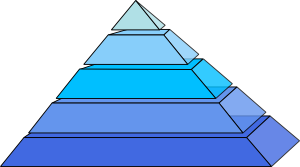
\includegraphics[width=1.1cm]{../Strukturfiler/FIGS/BluePyramid} & \begin{minipage}{\obsl}}{\end{minipage}\\ \end{tabular}\vspace{4mm}\newline}


% = Forudsætning = basis
\newenvironment{basis}{\begin{flushleft} \begin{itshape} }{\end{itshape} \end{flushleft}}


% = Opsummering =
\newenvironment{summary}{\clearpage\pagecolor{sumgul}\section{Opsummering}}{\newpage\pagecolor{white}}











% = Counter
\newcounter{opgavecount}[section]
\setcounter{opgavecount}{0}
\newcounter{spgcount}[opgavecount]
\setcounter{spgcount}{0}
\renewcommand{\thespgcount}{\alph{spgcount})}



% = EXERCISE = (DIVIDER)

\newcommand{\exercisebegin}[1][]{\bigskip\needspace{3\baselineskip}\refstepcounter{opgavecount}\titlegraphic{mingroen}\textcolor{mingroen}{\th{Opgave \theopgavecount \hspace*{1cm} #1}}\medskip\par}

% = QUIZEXERCISE = (DIVIDER)

\newcommand{\quizexercisebegin}[1][]{\bigskip\needspace{3\baselineskip}\refstepcounter{opgavecount}\titlegraphic{mingroen}\textcolor{mingroen}{\th{Quiz-Opgave \theopgavecount \hspace*{1cm} #1}}\medskip\par}

% = QUESTION =

\newenvironment{question}{\refstepcounter{spgcount}\begin{itemize}\item[\thespgcount]}{\end{itemize}\hspace*{\fill}}

% = VINK =

\newenvironment{vink}{\begin{tabular}{m{.9cm}<{\hspace*{2mm}}@{}|m{\obsl}@{}}\hspace*{-4pt}\raggedleft
\includegraphics[width=.9cm]{../Strukturfiler/FIGS/Think} & \begin{minipage}{\obsl}}{\end{minipage}\\ \end{tabular}\medskip\\}
	
% = FACIT =

\newenvironment{facit}{\begin{tabular}{m{.9cm}<{\hspace*{2mm}}@{}|m{\obsl}@{}}\hspace*{-4pt}\raggedleft
\includegraphics[width=.9cm]{../Strukturfiler/FIGS/Check} & \begin{minipage}{\obsl}}{\end{minipage}\\ \end{tabular}\medskip\\}








\newcommand{\afsnit}[1]{\bigskip\th{\titlegraphic{mingroen}\textcolor{mingroen}{#1}} \\ \rule[7pt]{.4\textwidth}{1pt} \vspace*{-2.5mm}\par}

% (DIVIDER):
\newcommand{\ugedagdatotitel}[4]{\pagebreak[4]\section{Semesteruge #1 -- #2 Dag \hspace*{1mm} (#3)} \vspace*{-4mm} \rule[5pt]{\textwidth}{1pt}\vspace*{-2.5mm} \begin{center}\large{\th{#4}}\end{center} \fancyhead[C]{\th{Semesteruge #1}}}

\newenvironment{skema}[1]{\definecolor{shadecolor}{rgb}{0.96,.98, 1.0} \setlength{\FrameSep}{6pt} \renewcommand{\FrameHeightAdjust}{10pt} \vspace*{-4pt}\begin{shaded} \begin{tabular}{#1}}{\end{tabular} \end{shaded} \vspace*{-7pt}}


% ========================

% MAKROER

%\newenvironment{matr}[1][]{\hspace*{-.8mm}\left[\hspace*{-1mm}\begin{array}{#1}}{\end{array}\hspace*{-1mm}\right]\hspace*{-.8mm}}
\newcommand{\bevisslut}{\begin{scriptsize} \begin{flushright} $ \blacksquare $ \end{flushright} \end{scriptsize}}

\newcommand{\tref}[2]{\hyperref[#1]{#2 \ref*{#1}}}
\newcommand{\thref}[2]{\hyperref[#1]{#2}}

\newcommand{\refA}[1]{\colorbox{yellow}{\ref{#1}}}
\newcommand{\hrefA}[2]{\colorbox{yellow}{\href{#1}{#2}}}
\newcommand{\trefA}[2]{\colorbox{yellow}{\hyperref[#1]{#2 \ref*{#1}}}}
\newcommand{\threfA}[2]{\colorbox{yellow}{\hyperref[#1]{#2}}}

\newenvironment{matr}[1]{\hspace*{-.8mm}\begin{bmatrix}\hspace*{-1mm}\begin{array}{#1}}{\end{array}\hspace*{-1mm}\end{bmatrix}\hspace*{-.8mm}}
\newcommand{\transp}{\hspace*{-.6mm}^{\top}}

\newcommand{\maengde}[2]{\left\lbrace \hspace*{-1mm} \begin{array}{c|c} #1 & #2 \end{array} \hspace*{-1mm} \right\rbrace}

\newenvironment{eqnalign}[1]{\setlength{\arraycolsep}{1.3pt}\begin{equation}\begin{array}{#1}}{\end{array}\end{equation}\par}
\newcommand{\eqnl}{\setlength{\arraycolsep}{1.3pt}}

\newcommand{\matind}[3]{{_\mathrm{#1}\mathbf{#2}_\mathrm{#3}}}
\newcommand{\vekind}[2]{{_\mathrm{#1}\mathbf{#2}}}
\newcommand{\jac}[2]{{\mathrm{Jacobi}_\mathbf{#1} (#2)}}
\newcommand{\diver}[2]{{\mathrm{div}\mathbf{#1} (#2)}}
\newcommand{\rot}[1]{{\mathbf{rot}\mathbf{(#1)}}}

\newcommand{\am}{\mathrm{am}}
\newcommand{\gm}{\mathrm{gm}}
\newcommand{\E}{\mathrm{E}}
\newcommand{\Span}{\mathrm{span}}
\newcommand{\mU}{\mathbf{U}}

\newcommand{\ms}{\medskip\\}
\newcommand{\bs}{\bigskip\\}

\newcommand{\mA}{\mathbf{A}}
\newcommand{\mB}{\mathbf{B}}
\newcommand{\mC}{\mathbf{C}}
\newcommand{\mD}{\mathbf{D}}
\newcommand{\mE}{\mathbf{E}}
\newcommand{\mF}{\mathbf{F}}
\newcommand{\mK}{\mathbf{K}}
\newcommand{\mI}{\mathbf{I}}
\newcommand{\mM}{\mathbf{M}}
\newcommand{\mN}{\mathbf{N}}
\newcommand{\mQ}{\mathbf{Q}}
\newcommand{\mT}{\mathbf{T}}
\newcommand{\mV}{\mathbf{V}}
\newcommand{\mW}{\mathbf{W}}
\newcommand{\mX}{\mathbf{X}}
\newcommand{\ma}{\mathbf{a}}
\newcommand{\mb}{\mathbf{b}}
\newcommand{\mc}{\mathbf{c}}
\newcommand{\md}{\mathbf{d}}
\newcommand{\me}{\mathbf{e}}
\newcommand{\mn}{\mathbf{n}}
\newcommand{\mr}{\mathbf{r}}
\newcommand{\mv}{\mathbf{v}}
\newcommand{\mw}{\mathbf{w}}
\newcommand{\mx}{\mathbf{x}}
\newcommand{\mxb}{\mathbf{x_{bet}}}
\newcommand{\my}{\mathbf{y}}
\newcommand{\mz}{\mathbf{z}}
\newcommand{\reel}{\mathbb{R}}
\newcommand{\mL}{\bm{\Lambda}} %Lambda-matrix
\newcommand{\mnul}{\bm{0}}
\newcommand{\trap}[1]{\mathrm{trap}(#1)}
\newcommand{\Det}{\operatorname{Det}}
\newcommand{\adj}{\operatorname{adj}}
\newcommand{\Ar}{\operatorname{Areal}}
\newcommand{\Vol}{\operatorname{Vol}}
\newcommand{\Rum}{\operatorname{Rum}}
\newcommand{\diag}{\operatorname{\bf{diag}}}
\newcommand{\bidiag}{\operatorname{\bf{bidiag}}}
\newcommand{\spanVec}[1]{\mathrm{span}\{#1\}}
\newcommand{\Div}{\operatorname{Div}}
\newcommand{\Rot}{\operatorname{\mathbf{Rot}}}

\newcommand{\Jac}{\operatorname{Jacobi}}
\newcommand{\Tan}{\operatorname{Tan}}
\newcommand{\Ort}{\operatorname{Ort}}
\newcommand{\Flux}{\operatorname{Flux}}
\newcommand{\Cmass}{\operatorname{Cm}}
\newcommand{\Imom}{\operatorname{Im}}
\newcommand{\Pmom}{\operatorname{Pm}}
\newcommand{\IS}{\operatorname{I}}
\newcommand{\IIS}{\operatorname{II}}
\newcommand{\IIIS}{\operatorname{III}}
\newcommand{\Le}{\operatorname{L}}
\newcommand{\app}{\operatorname{app}}
\newcommand{\M}{\operatorname{M}}
\newcommand{\re}{\mathrm{Re}}
\newcommand{\im}{\mathrm{Im}}

\newcommand{\compl}{\mathbb{C}} %de komplekse tal
\newcommand{\e}{\mathrm{e}} %eksponentialfunktionen. lodret 'e', og altså ikke kursiv ligesom andre bogstaver.





% Medialink: SCREEN: (QRcode) + thumbnail image + link på kodenummer (til qr.dtu.dk)
\newcommand{\onlinemedia}[3]{
	\begin{wrapfigure}{r}{3.2cm} 
		\vspace{-30pt} 
		\vspace{#1pt} 
		\begin{flushright} 
			\includegraphics[width=3cm]{qr/#2.png} 
			\tiny 
			\href{http://qr.dtu.dk/#2}{#2: #3}
			\normalsize  
		\end{flushright} 
		\vspace{-10pt} 
	\end{wrapfigure}
}
\newcommand{\onlinemediathumb}[3]{
	\begin{wrapfigure}{r}{3.2cm} 
		\vspace{-30pt} 
		\vspace{#1pt} 
		\begin{flushright} 
			\includegraphics[width=3cm]{qr/#2.png} 
			\includegraphics[width=3cm]{qr/#2_thumb.png} 
			\tiny 
			\href{http://qr.dtu.dk/#2}{#2: #3}
			\normalsize  
		\end{flushright} 
		\vspace{-10pt} 
	\end{wrapfigure}
}



% Index:
\usepackage{makeidx}
\makeindex
\newcommand\ind[2]{\index{#1}\textbf{\textit{\textcolor{black}{#2}}}}

% ###SERVER_EXCLUDE_BEGIN###
\externaldocument[NUID17-]{../../enoten/TN01-Talrum/Talrum}
\externaldocument[NUID1-]{../../enoten/TN02-Ligningssystemer/TNdriver}
\externaldocument[NUID2-]{../../enoten/TN03-Matricer_og_Matrixalgebra/Matricer_og_matrixalgebra}
\externaldocument[NUID3-]{../../enoten/TN04-Kvadratiske_matricer/TNdriver}
\externaldocument[NUID11-]{../../enoten/TN05-Determinanter/Determinanter}
\externaldocument[NUID12-]{../../enoten/TN06-GeometriskeVektorer/GeometriskeVektorer}
\externaldocument[NUID18-]{../../enoten/TN07-Vektorrum/VektorRum}
\externaldocument[NUID21-]{../../enoten/TN08-LinAfbildninger/LinAfbildninger}
\externaldocument[NUID23-]{../../enoten/TN09-Egenvaerdier_og_egenvektorer/TNdriver}
\externaldocument[NUID24-]{../../enoten/TN10-Diagonalisering_med_egenvektorer/TNdriver}
\externaldocument[NUID10-]{../../enoten/TN11-1.ordens_differentialligninger/TNdriver}
\externaldocument[NUID13-]{../../enoten/TN12-1.ordens_differentialligningssystemer/TNdriver}
\externaldocument[NUID14-]{../../enoten/TN13-2.ordens_differentialligninger/TNdriver}
\externaldocument[NUID27-]{../../enoten/TN14-Elemenataere_funktioner/Elementaere_Funktioner}
\externaldocument[NUID28-]{../../enoten/TN15-Funktioner2Variable/Funktioner_To_Variable}
\externaldocument[NUID29-]{../../enoten/TN16-Gradienter_og_Tangentplaner/Gradienter_og_Tangentplaner}
\externaldocument[NUID32-]{../../enoten/TN17-Taylor_formler/Taylor_Formler}
\externaldocument[NUID33-]{../../enoten/TN18-Taylor_2Var/Taylor_2Var}
\externaldocument[NUID34-]{../../enoten/TN19-SymMat/SymmetriskeMatricer}
\externaldocument[NUID35-]{../../enoten/TN20-KegleSnit/Keglesnit}
\externaldocument[NUID36-]{../../enoten/TN21-Riemann_Integral/Riemann_01}
\externaldocument[NUID37-]{../../enoten/TN22-Plan_Int/Plan_Int_01}
\externaldocument[NUID39-]{../../enoten/TN23-Flade_Int/Flade_Rum_Int_01}
\externaldocument[NUID40-]{../../enoten/TN24-Vektorfelter/Vektorfelter_01}
\externaldocument[NUID41-]{../../enoten/TN25-Flux/Flux_02}
\externaldocument[NUID42-]{../../enoten/TN26-Gauss/Gauss_01}
\externaldocument[NUID128-]{../../enoten/TN27-Stokes/Stokes_01}
\externaldocument[NUID43-]{../../enoten/TN29-KomplekseTal/KomplekseTal}

\externaldocument[NUID6-]{../../E-math-opgaver/Opgaver/opgU123}
\externaldocument[NUID19-]{../../E-math-opgaver/Opgaver/opgU45}
\externaldocument[NUID20-]{../../E-math-opgaver/Opgaver/opgU678}
\externaldocument[NUID25-]{../../E-math-opgaver/Opgaver/opgU910SD}
\externaldocument[NUID31-]{../../E-math-opgaver/OpgaverF11-U123/opgF123}
% \externaldocument[NUID9-]{../../E-math-opgaver/Opgaver/Dagsordner E10}
% ###SERVER_EXCLUDE_END###


% Begin document and set alternative chapter title:
\begin{document}
\renewcommand{\chaptername}{eNote}

\setcounter{chapter}{17} %SÆT DETTE TAL TIL 1 MINDRE END DET AKTUELLE TRANSFERNOTE-NUMMER!!

%%%%%%%%%%%%%%%%%%%%%%%%%%%%%%%%%%%%%%%%%%%%%
%%%%%%%%%%%%%%%%%%%%%%%%%%%%%%%%%%%%%%%%%%%%%
%%% HERFRA SKAL DU SKRIVE ELLER INDSÆTTE %%%%
%%% DEN FIL DU ØNSKER %%%%%%%%%%%%%%%%%%%%%%%
%%%%%%%%%%%%%%%%%%%%%%%%%%%%%%%%%%%%%%%%%%%%%
%%%%%%%%%%%%%%%%%%%%%%%%%%%%%%%%%%%%%%%%%%%%%


% REF: TransferNote \ref{TN4-tn4} \nameref{TN4-tn4}
%
% \tref{NUID14-thm.koma}{sætning}
%
% \tref{NUID28-tn15}{eNote}
%  \mathring{M}
%
% 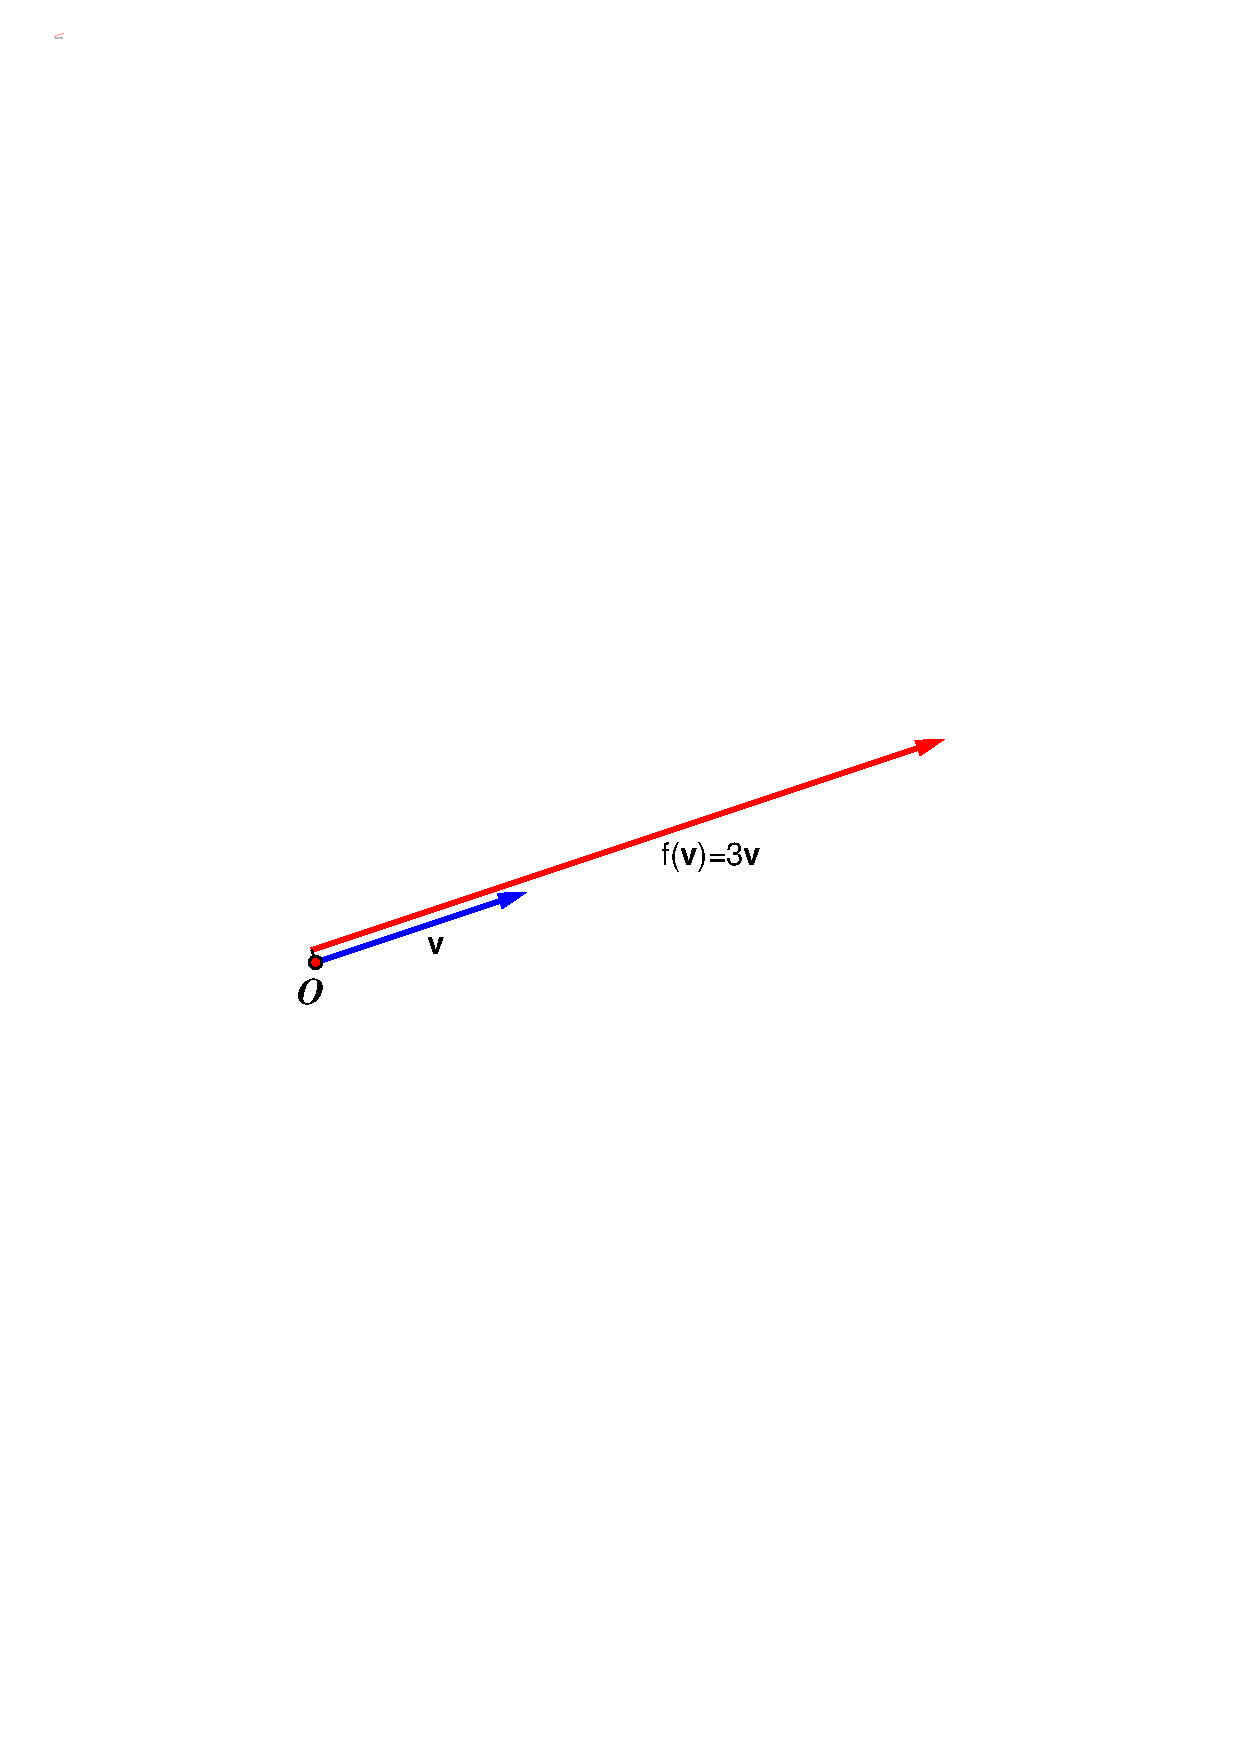
\includegraphics[trim=5cm 12cm 5cm 12cm,width=0.40\textwidth,clip]{skalering.pdf}
%
%
%

\chapter{Taylor's grænseformel for funktioner af to variable} \label{tn18}

\begin{basis}
 I \tref{NUID32-tn17}{eNote} har vi studeret Taylor's grænseformel for én variabel og fundet approksimerende polynomier af vilkårlig høj grad til givne funktioner. For funktioner af to variable gælder en tilsvarende formel, som vi dog vil nøjes med at udvikle til approksimation med andengrads-polynomier. Vi kan også her benytte Taylor's grænseformel til at undersøge funktionsværdierne i og omkring ethvert punkt hvor funktionen er glat. Specielt vil vi i første omgang benytte formlen for funktioner af to variable til at finde og undersøge lokale og globale minima og maksima for funktionerne.
\end{basis}

%%%%%%%%%%%%%%%%%%%%%%%%%%%%%%%%%%%%%%%%%%%%%%%%%%%%%%%%%%%%%
%%%%%%%%%%%%%%%%%%%%%%%%%%%%%%%%%%%%%%%%%%%%%%%%%%%%%%%%%%%%%
%%%%%%%%%%%%%%%%%%%%%%%%%%%%%%%%%%%%%%%%%%%%%%%%%%%%%%%%%%%%%



\section{Højere-ordens afledede} \label{secTaylor2Var}
Vi vil i denne eNote undersøge funktioner $f(x, y)$ af to variable i et område $M$ som er en delmængde af definitionsmængden for $f(x,y)$ i planen, $M \subset \mathcal{D}m(f) \subset \mathbb{R}^{2}$.\\


%%%%%%%%%%%%%%%%%%%%%%%%%%%%%%%%%%%%%%%%%%%%%%%%%%%%%%%%%%%%%
%%%%%%%%%%%%%%%%%%%%%%%%%%%%%%%%%%%%%%%%%%%%%%%%%%%%%%%%%%%%%
%%%%%%%%%%%%%%%%%%%%%%%%%%%%%%%%%%%%%%%%%%%%%%%%%%%%%%%%%%%%%



Vi vil antage, at funktionen kan differentieres partielt vilkårligt mange gange, altså at alle de afledede funktioner eksisterer for ethvert $(x,y)$ i det indre af $M$: $f'_{x}(x, y)$, $f'_{y}(x, y)$, $f''_{xx}(x, y)$, $f''_{xy}(x, y)$, $f''_{yy}(x, y)$, $f'''_{xyx}(x,y)$ osv. Disse højere afledede vil vi bruge til at konstruere (koefficienterne i) de approksimerende polynomier  af to variable præcis på samme måde som vi konstruerede dem for funktioner af \'{e}n variabel.

\begin{definition}
Hvis en funktion $f(x,y)$  kan differentieres partielt  vilkårligt mange gange i ethvert punkt $(x,y)$ i det indre $\mathring{M}$ af et givet område $M$ i planen, så siger vi, at funktionen er \ind{glat funktion}{glat} i $\mathring{M}$.
\end{definition}

\begin{example}[Højere-ordens afledede af nogle elementære funktioner] \label{exampDiffn}
Her er nogle første- og anden-ordens afledede af nogle kendte  funktioner af to variable. Læg mærke til, at $f''_{yx}(x,y)$ ikke optræder eksplicit i tabellen -- det er fordi $f''_{yx}(x,y)= f''_{xy}(x,y)$ for alle $(x,y)$ når funktionerne er glatte, som antaget, se \tref{NUID28-tn15}{eNote}. Funktionen $\rho_{(0,0)}(x,y) = \sqrt{x^{2} + y^{2}}$ betegner afstandsfunktionen fra $(0,0)$ til $(x,y)$; den er kun glat for $(x,y) \neq (0,0)$ som det også fremgår af de viste første- og anden-ordens partielle afledede af $\rho_{(0, 0)}(x,y)$ i tabellen. Funktionen $\rho_{(0,0)}^{2}(x,y) = x^{2} + y^{2}$ er derimod (som det også fremgår af tabellen) en glat funktion i hele definitionsområdet, dvs. for alle $(x,y) \in \mathbb{R}^{2}$. Det er kvadratet på afstanden fra et {\textit{vilkårligt punkt}} $(x_{0}, y_{0})$ tilsvarende også, dvs. funktionen: $$\rho_{(x_{0}, y_{0})}^{2}(x,y) = (x-x_{0})^{2} + (y-y_{0})^{2}\quad .$$

\begin{footnotesize}
\begin{equation*} \label{eqTabelHighOrderDeriv}
\begin{array}{|c|c|c|c|c|c|}
  \hline
  f(x,y) & f'_{x}(x,y) & f'_{y}(x,y) & f''_{xx}(x,y) & f''_{xy}(x,y) & f''_{yy}(x,y) \\ \hline \hline
    \e^{x} &  \e^{x} &  0&  \e^{x}& 0 &  0 \\ \hline
  \e^{x+y} &  \e^{x+y} &  \e^{x+y}&  \e^{x+y}& \e^{x+y} &  \e^{x+y} \\ \hline
   \e^{x^{2} + y^{2}} & 2\cdot x \cdot \e^{x^{2} + y^{2}} &   2\cdot y \cdot \e^{x^{2} + y^{2}}&  (2 + 4\cdot x^{2})\cdot\e^{x^{2} + y^{2}} & 4\cdot x \cdot y \cdot \e^{x^{2} + y^{2}}  &  (2+ 4\cdot y^{2})\cdot\e^{x^{2} + y^{2}}\\ \hline
   \e^{x\cdot y} & y\cdot\e^{x\cdot y} & x\cdot\e^{x\cdot y} & y^{2}\cdot \e^{x\cdot y}& \e^{x\cdot y}  +x \cdot y\cdot \e^{x\cdot y} &  x^{2}\cdot \e^{x\cdot y}\\ \hline
      \rho_{(0,0)}(x,y) & \frac{x}{\sqrt{x^{2} + y^{2}}} &  \frac{y}{\sqrt{x^{2} + y^{2}}} & \frac{y^{2}}{(x^{2} + y^{2})^{3/2}}  & -\frac{x\cdot y}{(x^{2} + y^{2})^{3/2}}   &   \frac{x^{2}}{(x^{2} + y^{2})^{3/2}}   \\ \hline
        \rho_{(0,0)}^{2}(x,y) & 2\cdot x &  2\cdot y & 2& 0& 2  \\ \hline
       \rho_{(x_{0}, y_{0})}^{2}(x,y)& 2\cdot (x-x_{0}) &  2\cdot (y-y_{0}) & 2 & 0& 2  \\ \hline \hline
\end{array}
\end{equation*}
\end{footnotesize}

\end{example}

I eksemplet \ref{exampDiffn} ovenfor er de partielle afledede sat på linje i tabellen. I det følgende vi\-ser det sig smart at {\textit{samle}} eller {\textit{pakke}}  de partielle afledede, dels de to første-ordens afledede til en vektor, gradientvektoren for $f(x,y)$ i $(x_{0}, y_{0})$, som også indføres og benyttes i \tref{NUID28-tn15}{eNote}:

\begin{equation}
\bm{\nabla}f(x_{0}, y_{0}) = (f'_{x}(x_{0}, y_{0}), f'_{y}(x_{0}, y_{0})) \quad ,
\end{equation}
og dels de tre anden-ordensafledede i en matrix $\mathbf{H}f(x_{0}, y_{0})$ -- den såkaldte Hesse-matrix for funktionen $f(x,y)$ i punktet $(x_{0}, y_{0})$, som er bestemt ved
\begin{equation}
\mathbf{H}f(x_{0}, y_{0}) = \left[
                              \begin{array}{cc}
                                f''_{xx}(x_{0}, y_{0}) & f''_{xy}(x_{0}, y_{0}) \\
                                f''_{yx}(x_{0}, y_{0}) & f''_{yy}(x_{0}, y_{0}) \\
                              \end{array}
                            \right] \quad .
\end{equation}

\begin{obs}
Bemærk specielt at denne matrix er symmetrisk fordi $f''_{xy}(x_{0}, y_{0}) = f''_{yx}(x_{0}, y_{0})$. Den har derfor nogle særlige egenskaber, som er afgørende i den geometriske analyse af funktioner til anden orden.
\end{obs}

\begin{example}[Gradienter og Hesse-matricer]\label{exampGradHessElem}
Ud fra tabellen aflæser vi følgende gradienter og Hesse-matricer for de givne elementære glatte funktioner i punktet $(x_{0}, y_{0})$:

\begin{center}
\begin{tabular}{|c|c|c|} \hline
$ f(x,y) $ & $ \bm{\nabla}f(x, y) $ & $ \mathbf{H}f(x, y) $ \\ \hline \hline
$ \e^{x} $ & $ (\e^{x}, 0) $ & $ \left[ \begin{array}{cc} \e^{x} & 0 \\ 0 & 0 \\ \end{array} \right] $ \\ \hline
$ \e^{x+y} $ & $ (\e^{x+y},\e^{x+y}) $ & $ \left[ \begin{array}{cc}\e^{x+y} & \e^{x+y} \\  \e^{x+y} & \e^{x+y} \\ \end{array} \right] $ \\ \hline
$ \rho^{2}_{(0,0)}(x,y) = x^{2} + y^{2} $ & $ (2\cdot x, 2 \cdot y) $ & $ \left[\begin{array}{cc} 2 & 0 \\  0 & 2 \\ \end{array}\right] $ \\ \hline
$ (x-x_{0}) \cdot \rho^{2}_{(x_{0}, y_{0})}(x,y) $ & \begin{minipage}{4.3cm} $ (3\cdot (x-x_{0})^{2} + (y-y_{0})^{2}, $ \\ $ 2 \cdot (x-x_{0})\cdot(y-y_{0})) $ \end{minipage} & $ \left[ \begin{array}{cc} 6\cdot (x-x_{0}) & 2\cdot(y-y_{0}) \\ 2\cdot(y-y_{0})  & 2\cdot(x-x_{0})  \\ \end{array} \right] $ \\ \hline \hline
\end{tabular}
\end{center}
\end{example}

\begin{aha}
Bemærk, at funktionen $f(x,y) = (x-x_{0}) \cdot \rho^{2}_{(x_{0}, y_{0})}(x,y)$ har gradientvektoren $\bm{0}$ og Hesse-matricen $\bm{0}$ når de udregnes i selve basispunktet $(x_{0}, y_{0})$ for afstandsfunktionen $\rho_{(x_{0}, y_{0})}(x,y)$.
\end{aha}


\begin{exercise}\label{exercGradHess}
Bestem gradienten $\bm{\nabla}f(x,y)$ og Hesse-matricen $\mathbf{H}f(x,y)$ i ethvert punkt $(x,y) \in \mathbb{R}^{2}$ for hver af følgende funktioner:
\begin{equation}
f(x,y)= \cos(x+y)\quad , \quad f(x,y)= \cos(x\cdot y)  \quad , \quad f(x,y)= x^{3} + y^{2} + x\cdot y \quad .
\end{equation}
\end{exercise}

\section{Approksimation af funktioner af to variable}

Vi vil nu sammenligne funktionen $f(x,y)$  med et vilkårligt andengrads-polynomium i de to variable $x$ og $y$ og bestemme koefficienterne i polynomiet ved at
kræve, at forskellen skal være lille i og omkring punktet $x_{0}$. \\

Det polynomium, vi vil afprøve og sammenligne med,
er følgende:
\begin{equation}
\begin{aligned}
a &+ b_{1}\cdot (x-x_{0}) + b_{2}\cdot (y-y_{0}) \\
&+ \left( \frac{h_{11}}{2}\right)\cdot (x-x_{0})^{2} + h_{12}\cdot (x-x_{0})\cdot (y-y_{0}) + \left(\frac{h_{22}}{2}\right) \cdot (y-y_{0})^{2} \quad .
\end{aligned}
\end{equation}

Vi vil vælge koefficienterne  $a$, $b_{1}$, $b_{2}$, $h_{11}$, $h_{12}$, og $h_{22}$,  så præcise at restfunktionen $R(x,y)= R_{2, (x_{0}, y_{0})}(x,y)$ i forhold til $f(x,y)$ bliver så (numerisk) lille som muligt i og omkring punktet $(x_{0}, y_{0})$ -- på samme måde som vi motiverede Taylor's formler for funktioner af \'{e}n variabel i \tref{NUID32-tn17}{eNote}:
\begin{equation} \label{eqTaylorRaw}
\begin{aligned}
f(x,y) = a
&+ b_{1}\cdot (x-x_{0}) + b_{2}\cdot (y-y_{0}) \\
&+ \left( \frac{h_{11}}{2}\right)\cdot (x-x_{0})^{2} + h_{12}\cdot (x-x_{0})\cdot (y-y_{0}) + \left(\frac{h_{22}}{2}\right) \cdot (y-y_{0})^{2} \\
&+ R(x,y) \quad .
\end{aligned}
\end{equation}

\begin{think}
Det polynomium af anden grad, som vi prøver at approksimere med i (\ref{eqTaylorRaw}), er et helt generelt andengradspolynomium; {\textit{ethvert}} andengradspolynomium kan skrives på denne form også selv om værdierne af $x_{0}$ og $y_{0}$ er givet på forhånd. Bemærk, at der er $6$ koefficienter, der endnu ikke er bestemt: $a$, $b_{1}$, $b_{2}$, $h_{11}$, $h_{12}$, og $h_{22}$. Og mængden af andengradspolynomier i to variable er netop et $6$-dimensionalt vektorrum! \\

Kunsten er at finde de bedste værdier af disse  $6$ koefficienter, således at $R(x,y)$ bliver numerisk lille i og tæt på punktet $(x_{0}, y_{0})$.
\end{think}

Restfunktionen $R(x,y)$ kan skrives som forskellen mellem $f(x,y)$ og polynomiet:
\begin{equation} \label{eqRestFunk}
\begin{aligned}
R(x,y) &= f(x,y) - a - b_{1}\cdot (x-x_{0}) - b_{2}\cdot (y-y_{0}) \\
&- \left(\frac{h_{11}}{2}\right)\cdot (x-x_{0})^{2} -  h_{12}\cdot (x-x_{0})\cdot (y-y_{0}) - \left(\frac{h_{22}}{2}\right)\cdot (y-y_{0})^{2} \quad.
\end{aligned}
\end{equation}

Vi vil nu stille følgende naturlige krav til restfunktionen --  krav som sikrer, at restfunktionen  er meget lille i og omkring $(x_{0}, y_{0})$ og dermed, at {\textit{polynomiet}} vi får frem på den måde er meget tæt på funktionen $f(x,y)$.\\

Det første krav er naturligvis, at restfunktionen er $0$ i $(x_{0}, y_{0})$.
Vi indsætter kravet i ligningen (\ref{eqRestFunk}) og får:
\begin{equation}
R(x_{0}, y_{0}) = 0 \quad \textrm{giver} \quad 0 = f(x_{0}, y_{0}) - a \quad,
\end{equation}
hvorved konstantleddet i det approksimerende polynomium allerede er bestemt:
\begin{equation}
a = f(x_{0}, y_{0}) \quad .\\
\end{equation}

Det næste krav er selvfølgelig at $R'_{x}(x_{0}, y_{0}) = R'_{y}(x_{0}, y_{0}) = 0$ således at $\bm{\nabla}R(x_{0}, y_{0}) = (0,0)$, hvilket geometrisk betyder, at grafen for restfunktionen har vandret tangentplan -- identisk med $(x,y)$-planen -- i $(x_{0}, y_{0})$.
Indsættes disse krav til $R(x,y)$ i ligningen (\ref{eqRestFunk}) får vi at
\begin{equation}
\begin{aligned}
R'_{x}(x_{0}, y_{0}) &= 0 \quad \textrm{som giver} \quad 0 = f'_{x}(x_{0}, y_{0}) - b_{1} \quad, \\ \\
R'_{y}(x_{0}, y_{0}) &= 0 \quad \textrm{som giver} \quad 0 = f'_{y}(x_{0}, y_{0}) - b_{2} \quad,
\end{aligned}
\end{equation}
hvorved koefficienterne $b_{1} = f'_{x}(x_{0}, y_{0})$ og $b_{2} = f'_{x}(x_{0}, y_{0})$ også er bestemte. Vi har:
\begin{equation}
(b_{1}, b_{2}) = \bm{\nabla}f(x_{0}, y_{0}) \quad.\\
\end{equation}

Det sidste krav til $R(x,y)$ vi vil anvende er at alle de tre anden-ordens partielle afledede af $R(x,y)$ også er $0$ i $(x_{0}, y_{0})$:

Indsættes disse $3$ krav til $R(x,y)$ i ligningen (\ref{eqRestFunk}) får vi at
\begin{equation}
\begin{aligned}
R''_{xx}(x_{0}, y_{0}) &= 0 \quad \textrm{som giver} \quad 0 = f''_{xx}(x_{0}, y_{0}) - h_{11} \quad, \\ \\
R''_{xy}(x_{0}, y_{0}) &= 0 \quad \textrm{som giver} \quad 0 = f''_{xy}(x_{0}, y_{0}) - h_{12} \quad, \\ \\
R''_{yy}(x_{0}, y_{0}) &= 0 \quad \textrm{som giver} \quad 0 = f''_{yy}(x_{0}, y_{0}) - h_{22} \quad.
\end{aligned}
\end{equation}
Dermed er de sidste $3$ koefficienter i det søgte polynomium fundet. \\

Vi kan skrive resultatet således -- når vi stadig husker på, at $f''_{xy}(x_{0}, y_{0}) = f''_{xy}(x_{0}, y_{0}) = h_{12}$:
\begin{equation}
\left[
  \begin{array}{cc}
    h_{11} & h_{12} \\
    h_{12} & h_{22}\\
  \end{array}
\right] = \left[
  \begin{array}{cc}
    f''_{xx}(x_{0}, y_{0}) & f''_{xy}(x_{0}, y_{0}) \\
    f''_{yx}(x_{0}, y_{0}) & f''_{yy}(x_{0}, y_{0})\\
  \end{array}
\right] = \mathbf{H}f(x_{0}, y_{0}) \quad .
\end{equation}

Vi har dermed indset, at de stillede krav til restfunktionen {\textit{kan opfyldes}}, og at
det resulterende andengradspolynomium, der opfylder kravene, derefter netop fortjener at blive kaldt {\textit{det approksimerende polynomium af anden grad}} for $f(x,y)$ med udviklingspunkt $(x_{0}, y_{0})$:

\begin{definition}[Approksimerende andengrads-polynomium]\label{defApp2Pol}
Lad $f(x,y)$ betegne en glat funktion i et område $M$ i $\mathbb{R}^{2}$ som indeholder punktet $(x_{0}, y_{0}) \in \mathring{M}$. Polynomiet
\begin{equation}
\begin{aligned}
P_{2, (x_{0}, y_{0})}(x,y) &= f(x_{0}, y_{0}) + f'_{x}(x_{0}, y_{0})\cdot (x-x_{0}) + f'_{y}(x_{0}, y_{0})\cdot (y-y_{0}) \\
&\phantom{abcdefghij}+ \frac{1}{2}\cdot f''_{xx}(x_{0}, y_{0})\cdot (x-x_{0})^{2}  \\
&\phantom{abcdefghij}+ f''_{xy}(x_{0}, y_{0})\cdot (x-x_{0})\cdot (y-y_{0}) \\
&\phantom{abcdefghij}+ \frac{1}{2} \cdot f''_{yy}(x_{0}, y_{0}) \cdot (y-y_{0})^{2}
\end{aligned}
\end{equation}
kaldes det \ind{approksimerende polynomium}{approksimerende polynomium} af anden grad for funktionen $f(x,y)$ med udviklingspunkt $(x_{0}, y_{0})$.
\end{definition}

Ligesom for funktioner af \'{e}n variabel er det nu rimeligt at forvente, at med de benyttede krav til restfunktionen $R(x,y) = R_{2, (x_{0}, y_{0})}(x,y)$  må den være numerisk sammenlignelig med en {\textit{potens af afstandsfunktionen}} $\rho_{(x_{0}, y_{0}})(x,y)$ til det betragtede punkt $(x_{0}, y_{0})$. For eksempel kan vi se af det sidste eksempel i \ref{exampGradHessElem} at alle de krav, vi har stillet til $R(x,y)$, er opfyldte for funktionen $(x-x_{0})\cdot \rho^{2}_{(x_{0}, y_{0})}(x,y)$.\\

Det er præcis indholdet af følgende sætning som udtrykker netop dette ved hjælp af en epsilonfunktion, som selvfølgelig sædvanligvis ikke er så simpel som $(x - x_{0})$:

\begin{lemma}[Restfunktion med epsilon-led]\label{lemmaRestfunk2var}
Givet en glat funktion $f(x,y)$. Så kan restfunktionen $R_{2, (x_{0}, y_{0})}(x,y)$  skrives på følgende form:
\begin{equation}
R_{2, (x_{0}, y_{0})}(x,y) = \rho^{2}_{(x_{0}, y_{0})}(x,y)\cdot \varepsilon_{f}(x-x_{0}, y-y_{0}) \quad ,
\end{equation}
hvor $\varepsilon_{f}(x-x_{0}, y-y_{0})$ er en epsilonfunktion af $(x-x_{0}, y-y_{0})$, dvs.
\begin{equation}
\varepsilon_{f}(x-x_{0}, y-y_{0}) \to 0 \quad \textrm{for} \quad (x, y) \to (x_{0}, y_{0}) \quad .
\end{equation}
\end{lemma}

Vi har nu alle ingredienserne til hovedsætningen i denne eNote:

\begin{theorem}[Taylor's grænseformel for funktioner af to variable] \label{thmTaylor2Var}
Enhver glat funktion $f(x,y)$ af to variable kan opdeles i et approksimerende andengrads-polynomium  med givet udviklingspunkt $(x_{0}, y_{0})$ og en restfunktion  med epsilon-led således:
\begin{equation} \label{eqTaylorLimit}
\begin{aligned}
f(x,y) &= P_{2, (x_{0}, y_{0})}(x,y) + R_{2, (x_{0}, y_{0})}(x,y) \\ \\
&= f(x_{0}, y_{0}) + f'_{x}(x_{0}, y_{0})\cdot (x-x_{0}) + f'_{y}(x_{0}, y_{0})\cdot (y-y_{0}) \\
&\phantom{abcdefghij}+ \frac{1}{2}\cdot f''_{xx}(x_{0}, y_{0})\cdot (x-x_{0})^{2}  \\
&\phantom{abcdefghij}+ f''_{xy}(x_{0}, y_{0})\cdot (x-x_{0})\cdot (y-y_{0}) \\
&\phantom{abcdefghij}+ \frac{1}{2} \cdot f''_{yy}(x_{0}, y_{0}) \cdot (y-y_{0})^{2} \\
&+\rho^{2}_{(x_{0}, y_{0})}(x,y)\cdot \varepsilon_{f}(x-x_{0}, y-y_{0}) \quad .
\end{aligned}
\end{equation}
\end{theorem}



Ved at bruge gradienten af $f(x,y)$ og Hesse-matricen for $f(x,y)$ kan vi skrive Taylor's grænseformel
(\ref{eqTaylorLimit}) på en mere kompakt form, som vi vil benytte i det følgende med henblik på den geometriske analyse  af $f(x,y)$ i og omkring udviklingspunktet $(x_{0}, y_{0})$:

\begin{theorem}[Taylor's grænseformel, kompakt, geometrisk]
Enhver glat funktion $f(x,y)$ af to variable er en sum af et approksimerende andengrads-polynomium med givet udviklingspunkt $(x_{0}, y_{0})$ og en restfunktion således:
\begin{equation} \label{eqTaylorLimitGeo}
\begin{aligned}
f(x,y) &= f(x_{0}, y_{0}) + \bm{\nabla}f(x_{0}, y_{0}) \bm{\cdot} (x-x_{0}, y-y_{0}) \\
&\phantom{abcdefghij}+ \frac{1}{2}\cdot \left[
                                          \begin{array}{cc}
                                            x-x_{0} & y-y_{0} \\
                                          \end{array}
                                        \right] \cdot \bm{H}f(x_{0}, y_{0})\cdot \left[
                                                                                   \begin{array}{c}
                                                                                         x-x_{0}  \\
                                                                                         y-y_{0}  \\
                                                                                   \end{array}
                                                                                 \right]\\
&\phantom{abcdefghij}+\rho^{2}_{(x_{0}, y_{0})}(x,y)\cdot \varepsilon_{f}(x-x_{0}, y-y_{0}) \quad ,
\end{aligned}
\end{equation}
hvor
\begin{equation}
\begin{aligned}
\bm{\nabla}f(x_{0}, y_{0}) &= (f'_{x}(x_{0}, y_{0}), f'_{y}(x_{0}, y_{0}))  \quad  \textrm{og} \\ \\
\mathbf{H}f(x_{0}, y_{0}) &= \left[
                              \begin{array}{cc}
                                f''_{xx}(x_{0}, y_{0}) & f''_{xy}(x_{0}, y_{0}) \\
                                f''_{yx}(x_{0}, y_{0}) & f''_{yy}(x_{0}, y_{0}) \\
                              \end{array}
                            \right] \quad .
\end{aligned}
\end{equation}
\end{theorem}
\begin{bevis}
En direkte udregningen af følgende matrixprodukt viser, at (\ref{eqTaylorLimitGeo}) er ækvivalent med
(\ref{eqTaylorLimit}), og det er det eneste nye i sætningen:
\begin{equation}
\begin{aligned}
& \left[
                                          \begin{array}{cc}
                                            x-x_{0} & y-y_{0} \\
                                          \end{array}
                                        \right] \cdot \bm{H}f(x_{0}, y_{0})\cdot \left[
                                                                                   \begin{array}{c}
                                                                                         x-x_{0}  \\
                                                                                         y-y_{0}  \\
                                                                                   \end{array}
                                                                                 \right] \\
& = \left[
                                          \begin{array}{cc}
                                            x-x_{0} & y-y_{0} \\
                                          \end{array}
                                        \right] \cdot  \left[
                              \begin{array}{cc}
                                f''_{xx}(x_{0}, y_{0}) & f''_{xy}(x_{0}, y_{0}) \\
                                f''_{yx}(x_{0}, y_{0}) & f''_{yy}(x_{0}, y_{0}) \\
                              \end{array}
                            \right] \cdot &\left[
                                                                                   \begin{array}{c}
                                                                                         x-x_{0}  \\
                                                                                         y-y_{0}  \\
                                                                                   \end{array}
                                                                                 \right] \\
&= \phantom{abcdefghij}f''_{xx}(x_{0}, y_{0})\cdot (x-x_{0})^{2}  \\
&\phantom{abcdefghij}+ 2 \cdot f''_{xy}(x_{0}, y_{0})\cdot (x-x_{0})\cdot (y-y_{0}) \\
&\phantom{abcdefghij}+ f''_{yy}(x_{0}, y_{0}) \cdot (y-y_{0})^{2} \quad .
\end{aligned}
\end{equation}
\end{bevis}

Det approksimerende andengrads-polynomium for $f(x,y)$ med udviklingspunkt $(x_{0}, y_{0})$ er derfor
på kompakt form:
\begin{equation}
\begin{aligned}
P_{2, (x_{0}, y_{0})}(x,y) &= f(x_{0}, y_{0}) + \bm{\nabla}f(x_{0}, y_{0}) \bm{\cdot} (x-x_{0}, y-y_{0}) \\
&+ \frac{1}{2}\cdot \left[
                                          \begin{array}{cc}
                                            x-x_{0} & y-y_{0} \\
                                          \end{array}
                                        \right] \cdot \bm{H}f(x_{0}, y_{0})\cdot \left[
                                                                                   \begin{array}{c}
                                                                                         x-x_{0}  \\
                                                                                         y-y_{0}  \\
                                                                                   \end{array}                                                                                \right] \quad .
\end{aligned}
\end{equation}

\begin{aha}
Læg mærke til, at det approksimerende førstegrads-polynomium for $f(x,y)$ net\-op er den {\textit{lineære del}} (lineariseringen) af det approksimerende anden\-grads\-po\-ly\-no\-mi\-um:
\begin{equation}
P_{1, (x_{0}, y_{0})}(x,y) = f(x_{0}, y_{0}) + \bm{\nabla}f(x_{0}, y_{0}) \bm{\cdot} (x-x_{0}, y-y_{0}).
\end{equation}
I \tref{NUID29-tn16}{eNote} har vi set, at den geometriske tolkning af $P_{1, (x_{0}, y_{0})}(x,y)$ er at
grafen for det approksimerende førstegrads-polynomium  $P_{1, (x_{0}, y_{0})}(x,y)$  (dvs. planen $z = P_{1, (x_{0}, y_{0})}(x,y)$ i $(x,y,z)$-rummet), netop er {\textit{tangentplanen til graf-fladen}} for $f(x,y)$ i punktet $(x_{0}, y_{0}, f(x_{0}, y_{0}))$.
\end{aha}

\begin{definition}[Stationære punkter for funktioner af to variable]\label{defStatPunkts}
Lad $f(x,y)$ betegne en glat funktion i et område $M$ i $\mathcal{D}m(f) \subset \mathbb{R}^{2}$.
Ved et \ind{stationært punkt}{stationært punkt} for $f(x,y)$ vil vi forstå ethvert punkt $(x_{0}, y_{0})$ i $\mathring{M}$ hvor gradienten for $f(x,y)$ er $(0, 0)$.\\

 I et stationært punkt for $f(x,y)$ har vi altså:
\begin{equation}
\bm{\nabla}f(x_{0}, y_{0}) = \left(f'_{x}(x_{0}, y_{0}), f'_{y}(x_{0}, y_{0}) \right) = (0, 0) \quad.
\end{equation}

\end{definition}

\begin{aha}
Geometrisk betyder definition \ref{defStatPunkts}, at $(x_{0}, y_{0})$ er et stationært punkt i $\mathring{M}$ for $f(x,y)$ hvis tangentplanen til grafen for $f(x,y)$ igennem punktet $(x_{0}, y_{0}, f(x_{0}, y_{0}))$ er vandret, altså  parallel med $(x,y)$-planen, således at enheds-normalvektoren til graf-fladen i punktet $(x_{0}, y_{0}, f(x_{0}, y_{0}))$ er $\mathbf{N}_{(x_{0}, y_{0})}(f) = (0,0,1)$.
\end{aha}


%%%%%%%%%%%%%%%%%%%%%%%%%%%%%%%%%%%%%%%%%%%%%%%%%%%%%%%%%%%%%
%%%%%%%%%%%%%%%%%%%%%%%%%%%%%%%%%%%%%%%%%%%%%%%%%%%%%%%%%%%%%
%%%%%%%%%%%%%%%%%%%%%%%%%%%%%%%%%%%%%%%%%%%%%%%%%%%%%%%%%%%%%



\section{Funktionsundersøgelser} \label{secFunkUnders}

Ligesom for kontinuerte funktioner af \'{e}n variabel gælder det for kontinuerte funktioner af to variable, at hvis det aktuelle område for funktionsundersøgelsen er tilstrækkelig pæn, så er funktionsværdierne $f(x,y)$ begrænsede i området:

\begin{theorem}[Hovedsætning for kontinuerte funktioner af to variable] \label{thmHovedsaetnKontTo}
Lad $f(x,y)$ betegne en funktion som er kontinuert i hele sin definitionsmængde $\mathcal{D}m(f) \subset \mathbb{R}^{2}$.
Lad $M$ være en begrænset, afsluttet, og sammenhængende mængde i $\mathcal{D}m(f)$. \\

Så er værdimængden for funktionen $f(x,y)$ i mængden $M$ et
begrænset, afsluttet, og sammenhængende interval $[\, A \, , \, B \, ] \subset \mathbb{R}$. Vi kan skrive således:
\begin{equation}
\mathcal{V}m(f_{|_{M}}) = f(M) = \{ f(x)\, | \, x\in M \} =  [\, A \, , \, B \, ] \quad ,
\end{equation}
hvor der stadig tillades den mulighed at $A = B$ og det sker naturligvis netop når $f(x,y)$ er konstant i hele $M$.
\end{theorem}

Præcis som for funktioner af \'{e}n variabel definerer vi nu:

\begin{definition} [Globalt minimum og globalt maksimum]
Når en funktion $f(x,y)$ har værdimængden $\mathcal{V}m(f_{|_{M}}) = f(M) = [\, A \, , \, B \, ]$ i en mængde $M$ siger vi, at
\begin{enumerate}
\item $A$ er den \ind{globale minimumværdi}{globale minimumværdi} for $f(x,y)$ i $M$, og hvis $f(x_{0}, y_{0})= A$ for $(x_{0}, y_{0}) \in M$ så er $(x_{0}, y_{0})$ et \ind{globalt minimumpunkt}{globalt minimumpunkt} for $f(x,y)$ i $M$.
\item $B$ er den \ind{globale maksimumværdi}{globale maksimumværdi} for $f(x,y)$ i $M$, og hvis $f(x_{0}, y_{0})= B$ for $(x_{0}, y_{0}) \in M$ så er $(x_{0}, y_{0})$ et \ind{globalt maksimumpunkt}{globalt maksimumpunkt} for $f(x,y)$ i $M$.
\end{enumerate}
\end{definition}

En helt naturlig og meget ofte forekommende opgave går ud på at finde de globale maksimum- og minimum-værdier for givne funktioner $f(x,y)$ i givne mængder og områder $M$ i $\mathbb{R}^{2}$ og samtidig dermed at bestemme de $(x,y)$-punkter i $M$  for hvilke
disse maksimum- og minimum-værdier {\textit{antages}} -- altså bestemme minimum- og maksimum-punkterne. \\

 For at løse den opgave er følgende igen en uvurderlig hjælp (på samme måde som ved undersøgelsen af funktioner af \'{e}n variabel):

\begin{lemma}[Maksima og minima i stationære punkter]\label{lemmaMaksMin2Var}
Lad $(x_{0}, y_{0})$ være et globalt maksimum- eller minimum-punkt for $f(x,y)$ i $M$. \\

 Antag, at  $(x_{0}, y_{0})$ ikke er et punkt på randen af området $M$, dvs. vi antager, at $(x_{0}, y_{0})$ er et indre punkt i $M$. Antag yderligere, at $f(x,y)$ er differentiabel i punktet $(x_{0}, y_{0})$.\\

 Så er
$(x_{0}, y_{0})$ et \ind{stationært punkt}{stationært punkt} for $f(x,y)$ i $(x_{0}, y_{0}) \in \mathring{M}$:
\begin{equation}
(f'_{x}(x_{0}, y_{0}), f'_{y}(x_{0}, y_{0})) = \bm{\nabla}f(x_{0}, y_{0}) = \mathbf{0} = (0,0) \quad .
\end{equation}
\end{lemma}
\begin{bevis}
Beviset følger det tilsvarende argument for funktioner af \'{e}n variabel. Kort fortalt: Hvis $\bm{\nabla}f(x_{0}, y_{0}) \neq (0,0)$ så {\textit{stiger}} funktionsværdierne effektivt i retningen $\bm{\nabla}f(x_{0}, y_{0})$ fra $(x_{0}, y_{0})$ og funktionsværdierne {\textit{aftager}} effektivt i den modsatte retning $-\bm{\nabla}f(x_{0}, y_{0})$ fra $(x_{0}, y_{0})$ og $(x_{0}, y_{0})$ kan i så fald hverken være et minimum- eller et maksimum-punkt.
\end{bevis}


Hermed har vi undersøgelsesmetoden for funktioner af to variable:

\begin{method}[Undersøgelsesmetode]\label{metodeVm2Var}
Lad $f(x,y)$ være en kontinuert funktion og $M$ et afsluttet, begrænset, og sammenhængende område i definitionsmængden $\mathcal{D}m(f) \subset \mathbb{R}^{2}$.\\

Maksimum- og minimum-værdierne for funktionen $f(x,y)$, altså $A$ og $B$ i værdimængden $[A, B]$ for $f(x,y)$ i $M$  findes ved at finde og sammenligne funktionsværdierne i følgende punkter:
\begin{enumerate}
\item Randpunkterne for mængden $M$.
\item Undtagelsespunkter, dvs. de punkter i det indre af $M$ hvor funktionen $f(x,y)$ {\textit{ikke}} er differentiabel.
\item De stationære punkter, dvs. samtlige de punkter $(x_{0}, y_{0})$ i det indre af $M$ hvor funktionen $f(x,y)$ {\textit{er}} differentiabel og $(f'_{x}(x_{0}, y_{0}), f'_{y}(x_{0}, y_{0}) = \bm{\nabla}f(x_{0}, y_{0}) = \mathbf{0} = (0,0) $.
\end{enumerate}
\end{method}

\begin{think}
Ved denne undersøgelsesmetode findes naturligvis ikke blot de globale maksimum- og minimum-værdier $A$ og $B$ men også de $(x,y)$-punkter i $M \subset \mathbb{R}^{2}$ for hvilke
det globale maksimum $B$ og det globale minimum $A$ {\textit{antages}}, altså maksimum- og minimum-punkterne i det aktuelle område.
\end{think}






\begin{example}[Funktionsundersøgelse, værdimængde]\label{exampUndersog2Var}
Lad $f(x,y) = 1 + x^{2} - x\cdot y^{2}$. Vi vil  undersøge funktionen i det afsluttede begrænsede cirkulære område $M$ i planen som er afgrænset af cirklen med radius $1$ og centrum i $(0, 0)$, se figur \ref{figCirkVaerdi}.
\begin{equation}
\bm{\nabla}f(x, y) = (2\cdot x + y^{2}, 2\cdot y \cdot x) \quad .
\end{equation}

Funktionen er differentiabel i hele sin definitionsmængde $\mathcal{D}m(f) = \mathbb{R}^{2}$. I det indre af $M$, som er den åbne cirkelskive med radius $1$ og centrum i $(0,0)$ har funktionen netop \'{e}t stationært punkt $(x_{0}, y_{0}) = (0, 0)$ og værdien af $f(x_{0}, y_{0})$ er $f(0,0) = 1$. Da der ikke er undtagelsespunkter for $f(x,y)$ i den åbne cirkelskive mangler vi blot at undersøge funktionen på randen af området, altså funktionsværdierne på cirklen med radius $1$ og centrum i $(0,0)$.
Vi parametriserer den aktuelle  cirkel i planen på sædvanlig måde:
\begin{equation}
\mathbf{r}(u) = (\cos(u), \sin(u)) \quad, \quad u \in [-\pi, \pi] \quad ,
\end{equation}
og indsætter cirklens punkter i funktionsudtrykket og får dermed følgende sammensatte funktion, som angiver funktionsværdierne på cirklen når $u$ gennemløber intervallet $[-\pi, \pi]$:
\begin{equation}
h(u) = f(\mathbf{r}(u)) = 1+ \cos^{2}(u) - \cos(u)\cdot\sin^{2}(u) \quad .
\end{equation}
Vi differentierer $h(u)$ og finder:
\begin{equation}
h'(u) = -\sin(u)\cdot(2\cdot \cos(u) + 3\cdot \cos^{2}(u) -1)
\end{equation}
som giver $h'(u) = 0$ for $u= 0$, $u= \pm\pi$, og $u= \pm\arccos(1/3)$. I disse stationære punkter for funktionen
$h(u)$ antager $h(u)$ værdierne: $h(0) = 2$, $h(\pm \pi) = 2$, og $h(\pm\arccos(1/3)) = 22/27$. \\

Ved at sammenligne alle kandidatværdierne for henholdsvis  maksimum- og minimumværdi for $f(x,y)$ som givet ved metoden \ref{metodeVm2Var} konkluderer vi, at værdimængden for $f(x,y)$ i den givne cirkelskive er:
\begin{equation}
f(M) = \left[\, \frac{22}{27}\, , \,  2\, \right] \quad,
\end{equation}
og maksimumpunkter og minimumpunkter findes alle på randen af cirkelområdet og er henholdsvis: maksimumpunkterne er  $(\cos(0), \sin(0)) = (1,0)$ og $(\cos(\pm\pi), \sin(\pm\pi)) = (-1,0)$ og minimumpunkterne er $(\cos(\pm\arccos(1/3)), \sin(\pm\arccos(1/3))) = (1/3, \pm 2\sqrt{2}/3)$.
\end{example}


\begin{figure}[ht]
\centerline{ 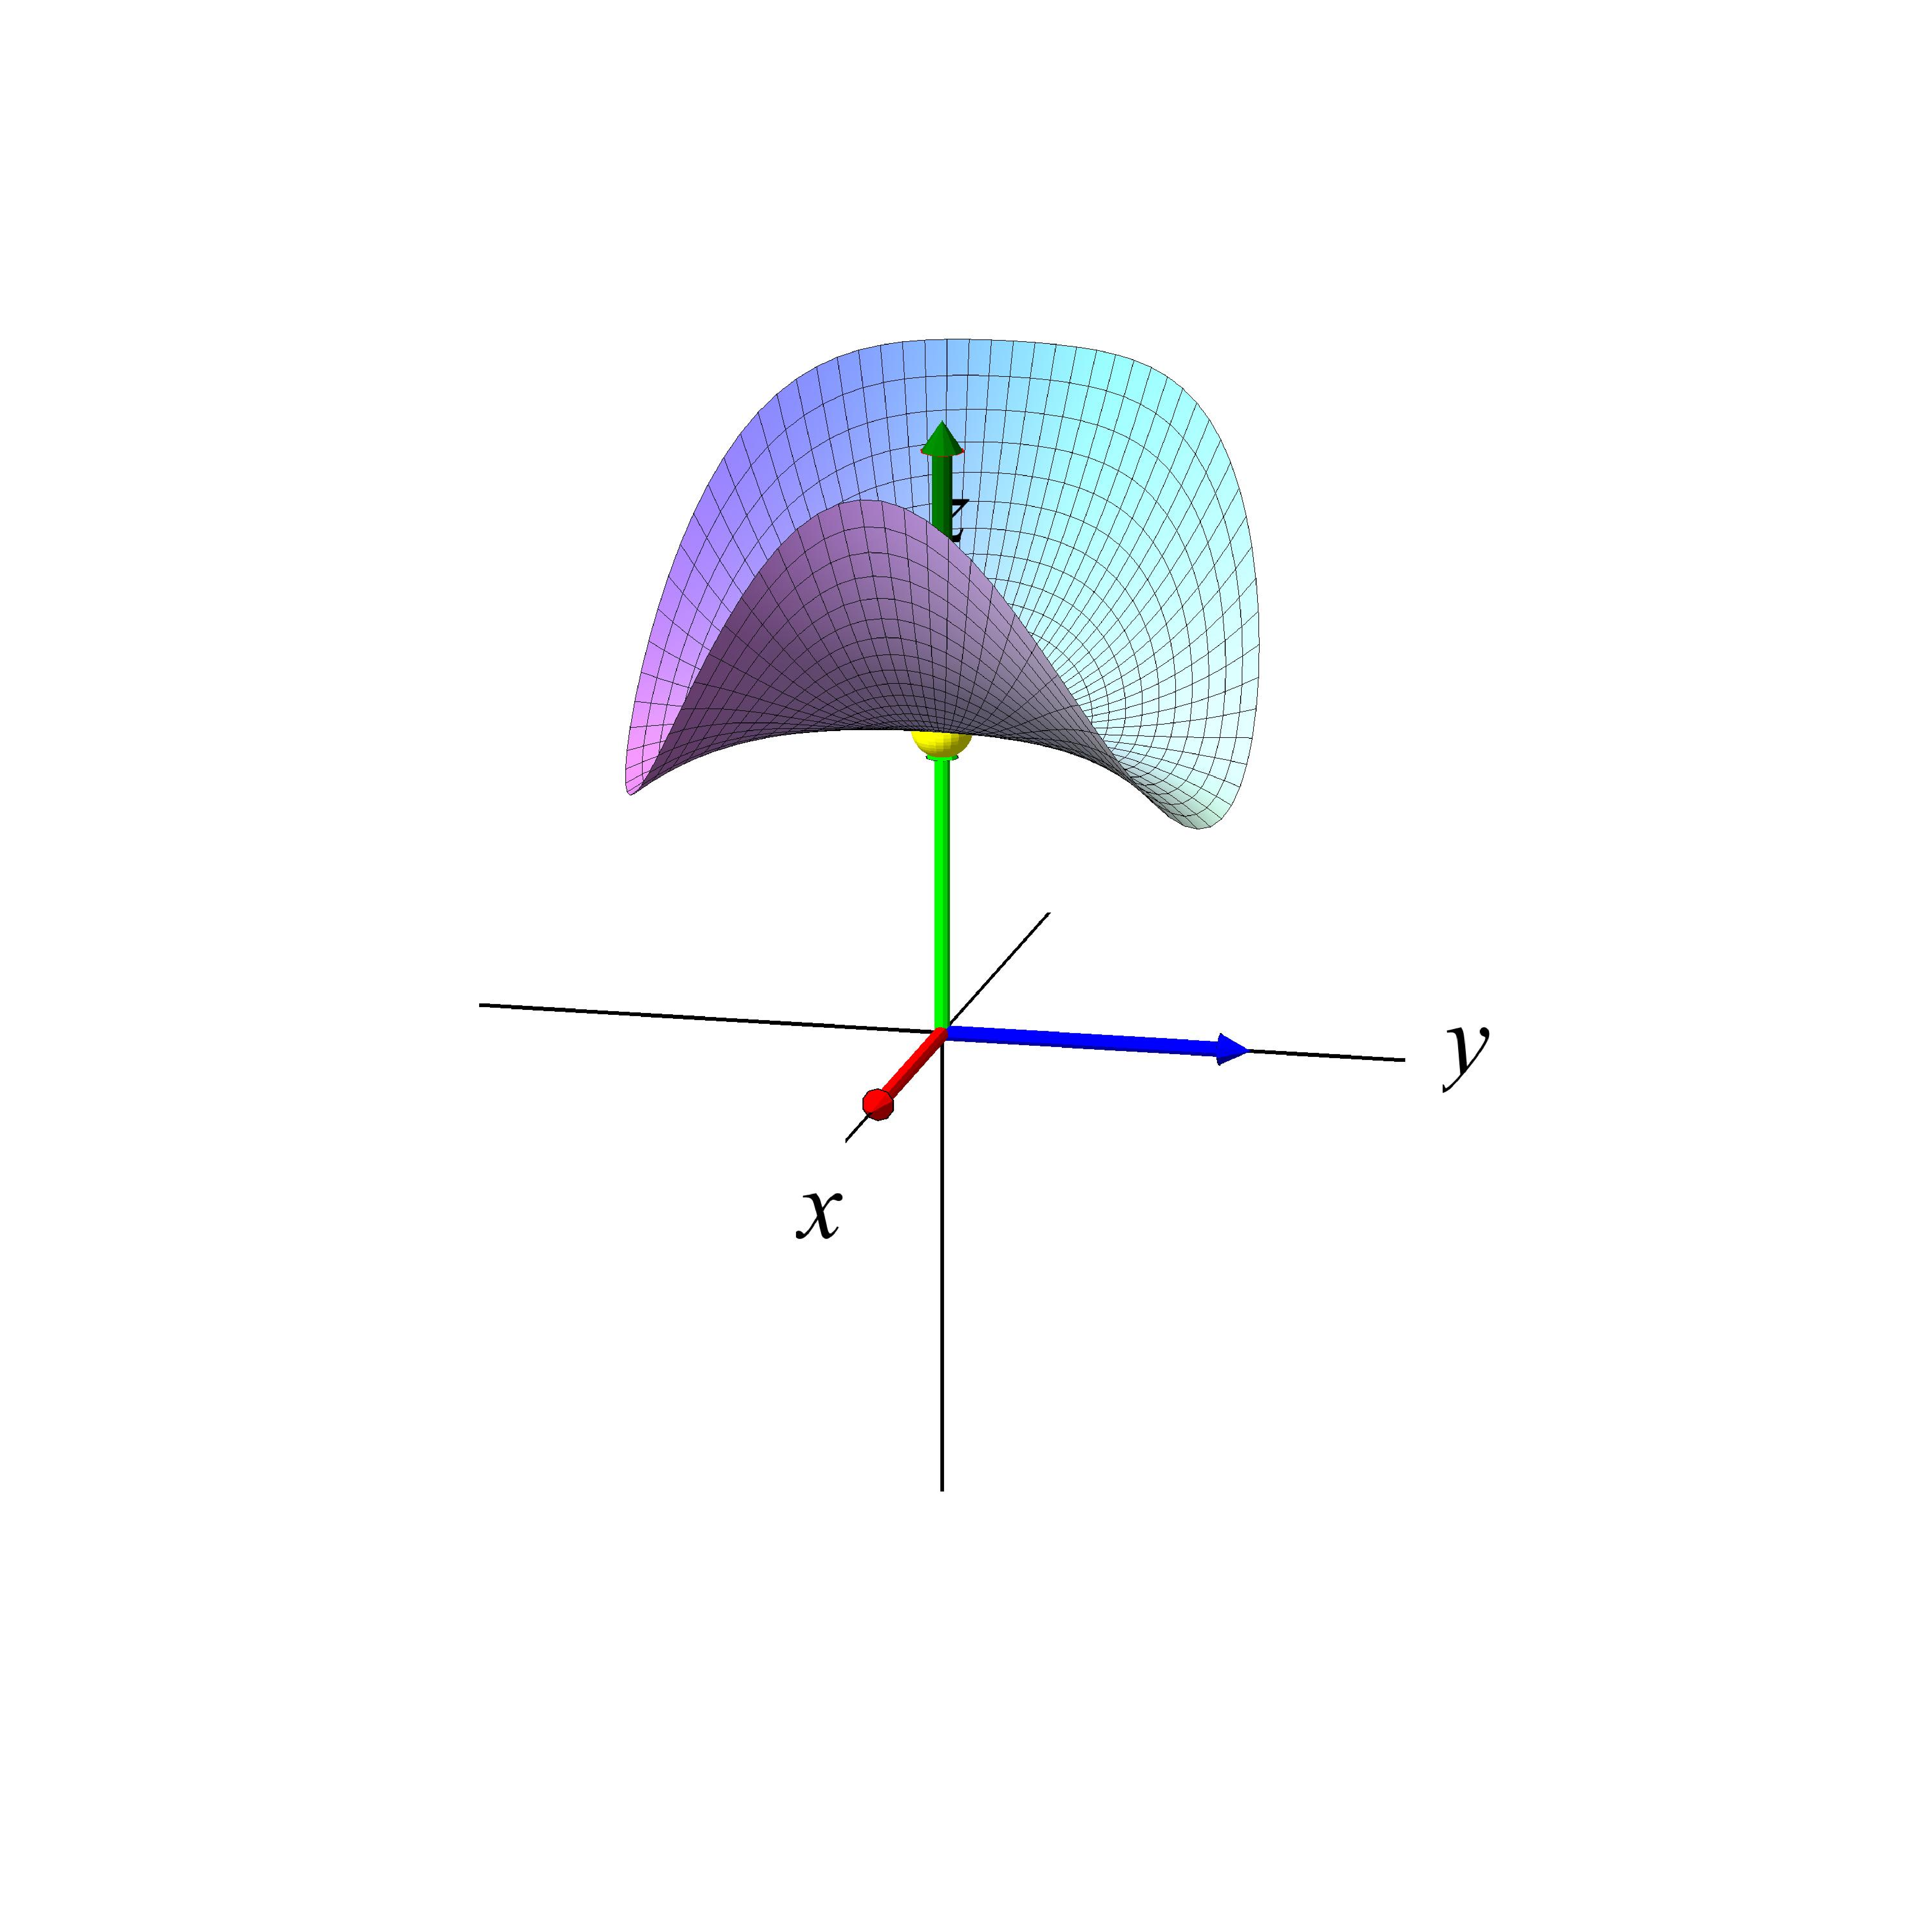
\includegraphics[height=75mm]{plotVar2Fig6.pdf} 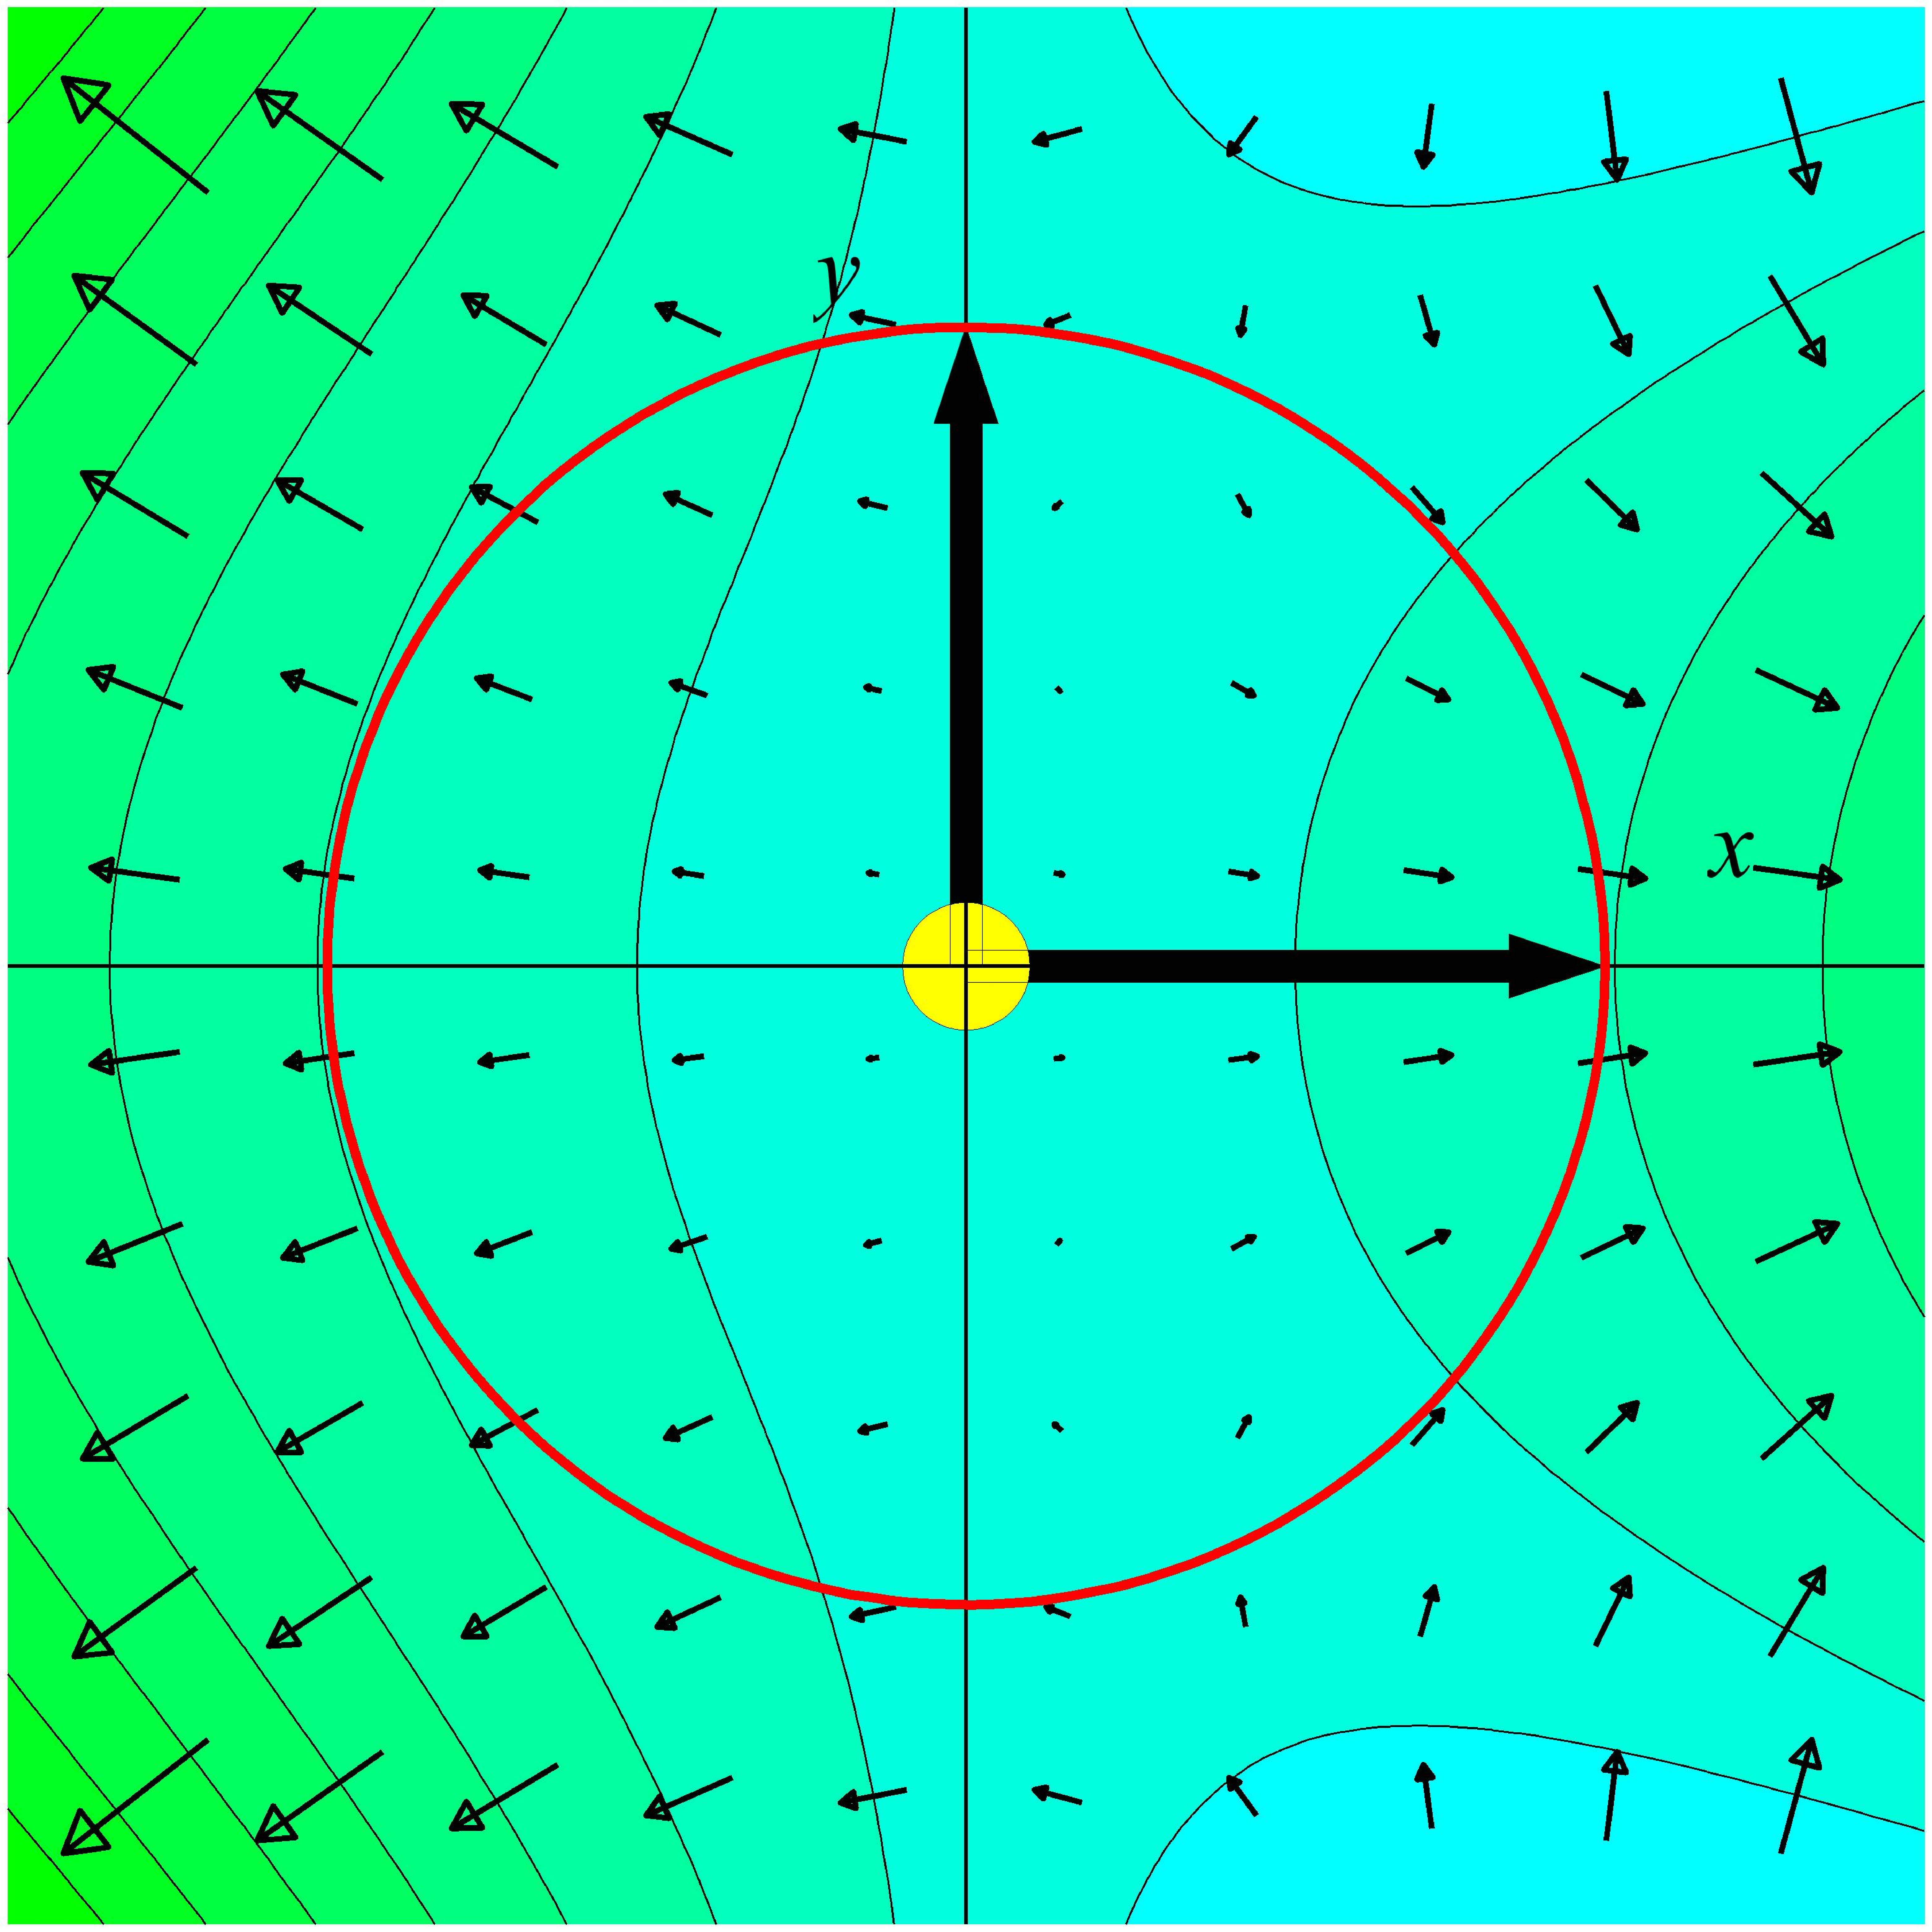
\includegraphics[height=75mm]{plotNivBdry6.pdf}}
\begin{center}
\caption{Grafen for funktionen $f(x,y)= 1 + x^{2} - x\cdot y^{2}$. Til højre inspiceres niveaukurver og gradientvektorfeltet for funktionen. Den røde cirkel er randen af det cirkulære område, der betragtes i eksempel \ref{exampUndersog2Var}. Det ses, at gradientvektorfeltet for $f(x,y)$ er {\textit{ortogonal på cirklen}} præcis i de $4$ fundne punkter hvor 'højde'-funktonen $h(u)$ har $h'(u)=0$ nemlig $(\pm 1,0)$ og $(1/3, \pm 2\sqrt{2}/3)$.} \label{figCirkVaerdi}
\end{center}
\end{figure}







\begin{definition}[Lokale minima og lokale maksima] \label{defLokMaxMin2Var}
Lad $f(x,y)$ betegne en funktion i et område $M$  som indeholder et givet indre punkt $(x_{0}, y_{0}) \in \mathring{M}$.
\begin{enumerate}
\item  Hvis $f(x,y) \geq f(x_{0}, y_{0})$ for alle $(x, y)$ i en (gerne lille) omegn om $(x_{0}, y_{0})$ dvs. for alle $(x, y)$ tilstrækkelig tæt på $(x_{0}, y_{0})$, så kaldes $f(x_{0}, y_{0})$ en  \ind{lokal minimumværdi}{lokal minimumværdi} for $f(x,y)$ i $M$, og $(x_{0}, y_{0})$ er et \ind{lokalt minimumpunkt}{lokalt minimumpunkt} for $f(x,y)$ i $M$. Hvis der faktisk gælder $f(x,y) > f(x_{0}, y_{0})$ for alle $(x, y)$ i omegnen fraregnet punktet $(x_{0}, y_{0})$ selv, så kaldes $f(x_{0}, y_{0})$ en \ind{egentlig lokal minimumværdi}{egentlig lokal minimumværdi}.
\item Hvis $f(x,y) \leq f(x_{0}, y_{0})$ for alle $(x,y)$ i en (gerne lille) omegn om $(x_{0}, y_{0})$, så kaldes $f(x_{0}, y_{0})$ en  \ind{lokal maksimumværdi}{lokal maksimumværdi} for $f(x,y)$ i $M$, og $(x_{0}, y_{0})$ er et \ind{lokalt maksimumpunkt}{lokalt maksimumpunkt} for $f(x,y)$ i $M$. Hvis der faktisk gælder at $f(x, y) < f(x_{0}, y_{0})$ for alle $(x,y)$ i omegnen (fraregnet $(x_{0}, y_{0})$ selv), så kaldes $f(x_{0}, y_{0})$ en \ind{egentlig lokal maksimumværdi}{egentlig lokal maksimumværdi}.
\end{enumerate}
\end{definition}


%%%%%%%%%%%%%%%%%%%%%%%%%%%%%%%%%%%%%%%%%%%%%%%%%%%%%%%%%%%%%
%%%%%%%%%%%%%%%%%%%%%%%%%%%%%%%%%%%%%%%%%%%%%%%%%%%%%%%%%%%%%
%%%%%%%%%%%%%%%%%%%%%%%%%%%%%%%%%%%%%%%%%%%%%%%%%%%%%%%%%%%%%




\section{Speciel undersøgelse i stationære punkter} \label{secSpecStat}


Hvis den funktion vi vil undersøge er glat i sine stationære punkter, så kan vi kvalificere metoden \ref{metodeVm2Var} endnu bedre, idet det approksimerende andengrads-polynomium med udviklingspunkt i et stationært punkt $(x_{0}, y_{0})$ kan hjælpe med at afgøre, om værdien af $f(x,y)$ i det stationære punkt er en kandidat til at være en global maksimumværdi eller global minimumværdi. \\

\begin{think}
Et egentligt lokalt minimumpunkt i det indre af $M$ kan begribeligvis ikke være et globalt maksimumpunkt for $f(x,y)$ i $M$ og et egentligt lokalt maksimumpunkt i det indre af $M$ kan ikke være et globalt minimumpunkt for $f(x,y)$ i $M$.
\end{think}

Til den lokale analyse af  $f(x,y)$ omkring et stationært punkt vil vi bruge {\textit{egenværdierne}} for Hesse-matricen $\mathbf{H}f(x_{0}, y_{0})$ for $f(x,y)$ i det
stationære punkt. Som nævnt er symmetrien af $\mathbf{H}f(x_{0}, y_{0})$ en vigtig egenskab, for som vi nu skal se betyder det, at $\mathbf{H}f(x_{0}, y_{0})$ kan {\textit{diagonaliseres ved en similartransformation}}, som indført og behandlet i  eNote 10. \\

Følgende sætning om symmetriske matricer er også helt central for rigtig mange andre anvendelser. Som det vises i eNote 19 kan resultatet generaliseres til vilkårlige symmetriske matricer. For $2 \times 2$-matricer er beviset rimelig simpelt, så vi går igennem begrundelserne nedenfor -- som en opvarmning til det generelle resultat.

\begin{theorem}[Diagonalisering af symmetriske $2\times 2$-matricer] \label{thmSymDiag}
Enhver  symmetrisk $2 \times 2$-matrix $\mathbf{A}$ har reelle egenværdier $\lambda_{1}$ og $\lambda_{2}$ og $\mathbf{A}$ kan diagonaliseres ved en $2 \times 2$-similartransformation $\mathbf{D}$ (basisskiftematrix) hvori de to søjlevektorer er ortogonale enheds-egenvektorer for $\mathbf{A}$. \\

Det betyder at $\mathbf{D}^{-1} = \mathbf{D}^{\top}$ og
\begin{equation}
\begin{aligned}
\bm{\Lambda} &= \left[
                 \begin{array}{cc}
                  \lambda_{1}& 0 \\
                   0 & \lambda_{2} \\
                 \end{array}
               \right] \quad , \\
\mathbf{A} &= \mathbf{D}\cdot \bm{\Lambda}\cdot \mathbf{D}^{-1} = \mathbf{D}\cdot \bm{\Lambda}\cdot \mathbf{D}^{\top}\quad , \textrm{og}\\
\bm{\Lambda} &= \mathbf{D}^{-1}\cdot \mathbf{A}\cdot \mathbf{D} = \mathbf{D}^{\top}\cdot \mathbf{A}\cdot \mathbf{D}\quad .
\end{aligned}
\end{equation}
\end{theorem}
\begin{bevis}
For det første kan vi direkte se, at enhver  symmetrisk $2 \times 2$-matrix har {\textit{reelle egenværdier}}: Det karakteristiske polynomium for den symmetriske matrix
\begin{equation}
\mathbf{A} = \left[
               \begin{array}{cc}
                 a & b \\
                 b & c \\
               \end{array}
             \right]
\end{equation}
 er
\begin{equation}
\mathbf{K}_{\mathbf{A}}(\lambda) = (a-\lambda)\cdot(c-\lambda) - b^{2} = \lambda^{2} - \lambda\cdot (a + c) + (a\cdot c - b^{2})  \quad ,
\end{equation}
der har rødderne (egenværdierne)
\begin{equation}
\begin{aligned}
\lambda_{1} &= \frac{1}{2}\left(a + c + \sqrt{(a-c)^{2} + 4\cdot b^{2} }  \right)  \quad \textrm{og} \\  \lambda_{2} &=   \frac{1}{2}\left(a + c - \sqrt{(a-c)^{2} + 4\cdot b^{2}} \right) \quad ,
\end{aligned}
\end{equation}
som begge er reelle tal. \\

De to egenværdier er ens netop når $a=c$ og $b=0$, dvs. når $\mathbf{A}$ allerede {\textit{er}} på diagonalform
og er et produkt af enhedsmatricen -- muligvis $\mathbf{0}$-matricen. I de tilfælde kan vi vælge $\mathbf{D}= \mathbf{E}$. \\

Hvis $\lambda_{1} \neq \lambda_{2}$ får vi også direkte fra eNote 10, sætning 10.4, at der {\textit{findes}} en similartransformation $\mathbf{D}$ der diagonaliserer $\mathbf{A}$:
\begin{equation}
\bm{\Lambda} = \mathbf{D}^{-1}\cdot \mathbf{A}\cdot \mathbf{D} \quad .
\end{equation}
Søjlevektorerne i $\mathbf{D}$ er egenvektorer $\mathbf{v}_{1}$ og $\mathbf{v}_{2}$ hørende til henholdsvis $\lambda_{1}$ og  $\lambda_{2}$.\\

Vi vil vise, at $\mathbf{v}_{1}$ og $\mathbf{v}_{2}$ er ortogonale vektorer. Da $\mathbf{A}$ er symmetrisk har vi
\begin{equation} \label{eqSymmetriskA}
\mathbf{v}_{1}\bm{\cdot} \left(\mathbf{A} \mathbf{v}_{2}\right)  = \mathbf{v}_{2}\bm{\cdot} \left(\mathbf{A} \mathbf{v}_{1} \right) \quad;
\end{equation}
det kan ses ved en direkte udregning med vilkårlige vektorer $\mathbf{v}_{1}$ og $\mathbf{v}_{2}$.

Da $\mathbf{v}_{1}$ er en egentlig egenvektor for $\mathbf{A}$ hørende til $\lambda_{1}$ og tilsvarende $\mathbf{v}_{2}$ er en egentlig egenvektor for $\mathbf{A}$ hørende til $\lambda_{2}$ har vi derfor:
\begin{equation}
\begin{aligned}
\mathbf{A} \mathbf{v}_{2} &= \lambda_{2} \cdot \mathbf{v}_{2} \\
\mathbf{A} \mathbf{v}_{1} &= \lambda_{1} \cdot \mathbf{v}_{1} \quad ,
\end{aligned}
\end{equation}
som indsat i (\ref{eqSymmetriskA}) giver:
\begin{equation}
\lambda_{2} \cdot \mathbf{v}_{1}\bm{\cdot} \mathbf{v}_{2} = \lambda_{1} \cdot \mathbf{v}_{2}\bm{\cdot} \mathbf{v}_{1} \quad ,
\end{equation}
således at
\begin{equation}
 (\mathbf{v}_{1}\bm{\cdot} \mathbf{v}_{2})\cdot(\lambda_{1} - \lambda_{2}) = 0 \quad .
\end{equation}
Da $\lambda_{1} \neq \lambda_{2}$  kan denne ligning kun være opfyldt for $\mathbf{v}_{1}\bm{\cdot} \mathbf{v}_{2} = 0$.
De to egenvektorer er altså ortogonale som påstået i sætningen.

Vi kan dernæst gerne antage, at de to egenvektorer $\mathbf{v}_{1}$ og $\mathbf{v}_{2}$ er enhedsvektorer -- ellers dividerer vi blot med deres respektive længder, og det ændrer ikke deres ''egenvektor-egenskab''.  \\

De to enhedsegenvektorer benyttes som søjlevektorerne i similartransformationsmatricen $D$, som dermed opfylder følgende ligning :
\begin{equation}
\mathbf{D}^{\top}\cdot \mathbf{D} = \mathbf{E} \quad  ,
\end{equation}
og dermed
\begin{equation}
\mathbf{D}^{\top} = \mathbf{D}^{-1}
\end{equation}
som ønsket og påstået i sætningen .

\end{bevis}

Specielt er egenværdierne for Hesse-matricen altid to reelle tal og det er disse egenværdier vi nu vil benytte som hjælp til at afgøre, om et givet stationært punkt er et egentligt maksimum- eller minimum-punkt.

\begin{lemma}[Lokal analyse omkring et stationært punkt] \label{lemmaEkstrema2Var}
Lad $f(x,y)$ være en glat funktion og antag, at $(x_{0}, y_{0})$ er et stationært punkt for $f(x,y)$ i et åbent område $\mathring{M} \subset \mathcal{D}m(f) \subset \mathbb{R}^{2}$. Lad $\lambda_{1}(x_{0}, y_{0})$ og $\lambda_{2}(x_{0}, y_{0})$ betegne egenværdierne for Hesse-matricen for $f(x,y)$ i $(x_{0}, y_{0})$.
Så gælder følgende:
\begin{enumerate}
\item Hvis $\lambda_{1}(x_{0}, y_{0}) > 0 $ og $\lambda_{2}(x_{0}, y_{0}) >0$  så er  $f(x_{0}, y_{0})$ en egentlig lokal minimumværdi for $f(x,y)$ .
\item Hvis $\lambda_{1}(x_{0}, y_{0}) < 0 $ og $\lambda_{2}(x_{0}, y_{0}) <0$ så er $f(x_{0}, y_{0})$ en egentlig lokal maksimumværdi for $f(x,y)$.
\item Hvis $\lambda_{1}(x_{0}, y_{0})\cdot \lambda_{2}(x_{0}, y_{0}) < 0 $ så er $f(x_{0}, y_{0})$ hverken  lokal minimumværdi eller lokal maksimumværdi for $f(x,y)$.
\item Hvis $\lambda_{1}(x_{0}, y_{0})\cdot \lambda_{2}(x_{0}, y_{0}) =  0 $ så er dette ikke tilstrækkelig information til at sikre at $f(x_{0}, y_{0})$ er lokal minimumværdi eller lokal maksimumværdi for $f(x,y)$.
\end{enumerate}
\end{lemma}

\begin{bevis}
Fra Taylor's grænseformel har vi i det stationære punkt følgende fremstilling af $f(x,y)$:
\begin{equation}
f(x,y) = f(x_{0}, y_{0}) + \frac{1}{2}\cdot \left[
                                          \begin{array}{cc}
                                            x-x_{0} & y-y_{0} \\
                                          \end{array}
                                        \right] \cdot \mathbf{H}f(x_{0}, y_{0})\cdot \left[
                                                                                   \begin{array}{c}
                                                                                         x-x_{0}  \\
                                                                                         y-y_{0}  \\
                                                                                   \end{array}                                                                                \right] + R_{2}(x,y) \,.
\end{equation}
Vi diagonaliserer $\bm{H}f(x_{0}, y_{0})$ med similartransformationen $\mathbf{D}$, jvf. sætning \ref{thmSymDiag}, sådan at
\begin{equation}
\begin{aligned}
&f(x,y) = f(x_{0}, y_{0}) + \frac{1}{2}\cdot \left[
                                          \begin{array}{cc}
                                            x-x_{0} & y-y_{0} \\
                                          \end{array}
                                        \right] \cdot \mathbf{D}\cdot\ \left[
                                                                               \begin{array}{cc}
                                                                                 \lambda_{1} & 0 \\
                                                                                 0 & \lambda_{2} \\
                                                                               \end{array}
                                                                             \right] \cdot
                                          \mathbf{D}^{-1}  \cdot \left[
                                                                                   \begin{array}{c}
                                                                                         x-x_{0}  \\
                                                                                         y-y_{0}  \\
                                                                                   \end{array}                                                                                \right] + R_{2}(x,y)\\
&= f(x_{0}, y_{0}) + \frac{1}{2}\cdot \left( \left[
                                          \begin{array}{cc}
                                            x-x_{0} & y-y_{0} \\
                                          \end{array}
                                        \right] \cdot \mathbf{D}\right)\cdot\ \left[
                                                                               \begin{array}{cc}
                                                                                 \lambda_{1} & 0 \\
                                                                                 0 & \lambda_{2} \\
                                                                               \end{array}
                                                                             \right] \cdot
                                         \left( \mathbf{D}^{\top}  \cdot \left[
                                                                                   \begin{array}{c}
                                                                                         x-x_{0}  \\
                                                                                         y-y_{0}  \\
                                                                                   \end{array}                                                                                \right] \right) + R_{2}(x,y) \quad ,
\end{aligned}
\end{equation}
hvor vi bemærker, at følgende to vektorer er ens (pånær transponeringen)
\begin{equation}
\left( \left[
                                          \begin{array}{cc}
                                            x-x_{0} & y-y_{0} \\
                                          \end{array}
                                        \right] \cdot \mathbf{D}\right)^{\top} =
                                         \left( \mathbf{D}^{\top}  \cdot \left[
                                                                                   \begin{array}{c}
                                                                                         x-x_{0}  \\
                                                                                         y-y_{0}  \\
                                                                                   \end{array}                                                                                \right] \right) = \left[
                                                                                                       \begin{array}{c}
                                                                                                         \alpha \\
                                                                                                         \beta \\
                                                                                                       \end{array}
                                                                                                     \right] \quad .
\end{equation}
Det vil sige vi kan skrive på kort form:
\begin{equation} \label{eqAlpBet}
\begin{aligned}
f(x,y) &= f(x_{0}, y_{0}) + \frac{1}{2}\cdot \left[
                                          \begin{array}{cc}
                                            \alpha & \beta \\
                                          \end{array}
                                        \right] \cdot\ \left[
                                                                               \begin{array}{cc}
                                                                                 \lambda_{1} & 0 \\
                                                                                 0 & \lambda_{2} \\
                                                                               \end{array}
                                                                             \right]  \cdot \left[
                                                                                   \begin{array}{c}
                                                                                         \alpha  \\
                                                                                         \beta  \\
                                                                                   \end{array}                                                                                \right] + R_{2}(x,y) \\
&= f(x_{0}, y_{0}) + \frac{1}{2}\cdot \left( \lambda_{1}\cdot \alpha^{2} + \lambda_{2}\cdot \beta^{2} \right) + R_{2}(x,y)
\end{aligned}
\end{equation}
Hvis både  $\lambda_{1}$  og  $\lambda_{2}$ er positive og $\lambda_{1} \geq \lambda_{2} >0 $ fås direkte heraf at:

\begin{equation}
 f(x,y) \geq f(x_{0}, y_{0}) + \lambda_{2}\cdot \left( \alpha^{2} + \beta^{2} \right) + R_{2}(x,y) \quad .
\end{equation}
Men vi har også, at $\alpha^{2} + \beta^{2} = (x-x_{0})^{2} + (y-y_{0})^{2}$ fordi $\mathbf{D}$ er så skikkelig:
\begin{equation}
\begin{aligned}
\alpha^{2} + \beta^{2} &=  \left(\left[
                                          \begin{array}{cc}
                                            \alpha & \beta \\
                                          \end{array}
                                        \right]\cdot \mathbf{D}^{\top}\right)  \cdot \left(\mathbf{D} \cdot \left[
                                                                                   \begin{array}{c}
                                                                                         \alpha  \\
                                                                                         \beta  \\
                                                                                   \end{array}                                                                                \right]\right) \\
&= \left[
                                          \begin{array}{cc}
                                            x-x_{0} & y-y_{0} \\
                                          \end{array}
                                        \right]\cdot \left[
                                                                                   \begin{array}{c}
                                                                                         x- x_{0}  \\
                                                                                         y-y_{0}  \\
                                                                                   \end{array}                                                                                \right] \\
&= (x-x_{0})^{2} + (y-y_{0})^{2}  \\
&= \rho^{2}_{(x_{0}, y_{0})}(x,y) \quad .
\end{aligned}
\end{equation}
Hvis vi dernæst indfører restfunktionen $R_{2}(x,y)$ med epsilon-led, får vi sluttelig:
\begin{equation}
f(x,y) \geq f(x_{0}, y_{0}) +  \rho^{2}_{(x_{0}, y_{0})}(x,y) \cdot (\lambda_{2} + \varepsilon_{f}(x-x_{0}, y-y_{0})) \quad.
\end{equation}
Vi kan hermed konkludere, at for  alle $(x,y)$ tilstrækkelig tæt på (men forskellig fra) udviklingspunktet $(x_{0}, y_{0})$ er
$f(x,y) > f(x_{0}, y_{0})$ fordi $\lambda_{2} >0$ og $\varepsilon_{f}(x-x_{0}, y-y_{0}) \to 0$ for $(x,y) \to (x_{0}, y_{0})$. \\

Tilsvarende kan naturligvis sluttes, at $f(x,y) < f(x_{0}, y_{0})$ for  alle punkter $(x,y)$ tilstrækkeligt tæt på (men forskellig fra) $(x_{0}, y_{0})$ hvis begge egenværdierne er negative. \\

Hvis $\lambda_{1} > 0 $ og  $\lambda_{2} <0 $  så kan vi benytte (\ref{eqAlpBet}) direkte med $\beta = 0$ henholdsvis $\alpha = 0$  og derved opnå værdier af $f(x,y)$ som er større henholdsvis mindre end $f(x_{0}, y_{0})$ for de tilsvarende punkter $(x,y)$ tilstrækkeligt tæt på (men forskellig fra) $(x_{0}, y_{0})$ således at $f(x_{0}, y_{0})$ ikke kan være hverken lokal minimum- eller maksimum-værdi. Tilsvarende konklusion fås på samme måde for
$\lambda_{1} < 0 $ og  $\lambda_{2} > 0$.
Og det var det, vi skulle vise.
\end{bevis}


\begin{think}
Man kunne måske forledes til at tro, at hvis blot alle andenordens-afledede af $f(x,y)$ er positive i et stationært punkt $(x_{0}, y_{0})$ så må funktionen have et egentligt minimumpunkt i $(x_{0}, y_{0})$. Men {\textit{så}} simpelt er det ikke. For eksempel har følgende Hesse-matrix ikke positive egenværdier selv om alle elementerne er positive:
\begin{equation}
\mathbf{H}f(x,y) = \left[
  \begin{array}{cc}
    1 & 2 \\
    2 & 1 \\
  \end{array}
\right] \quad .
\end{equation}
Egenværdierne er henholdsvis  $\lambda_{1} = 3$ og $\lambda_{2} = -1$, så ifølge hjælpesætningen \ref{lemmaEkstrema2Var} kan vi konkludere, at  eventuelt stationært punkt for $f(x,y)$ ikke er hverken et lokalt  maksimum- eller minimum-punkt for $f(x,y)$.\\

Den viste matrix er den {\textit{konstante}} Hesse-matrix for funktionen
\begin{equation}
f(x,y)= \frac{1}{2}\cdot \left(x^{2} + y^{2} + 4\cdot x \cdot y\right) \quad .
 \end{equation}
 Funktionen har klart et stationært punkt i $(x_{0}, y_{0}) = (0,0)$ men tydeligvis ikke noget egentligt minimumpunkt i $(0,0)$,  som det også fremgår af figur \ref{figPosHess}. Den betragtede funktion er sit eget approksimerende polynomium af anden grad med udviklingspunkt i $(0,0)$.
\end{think}

\begin{figure}[ht]
\centerline{ 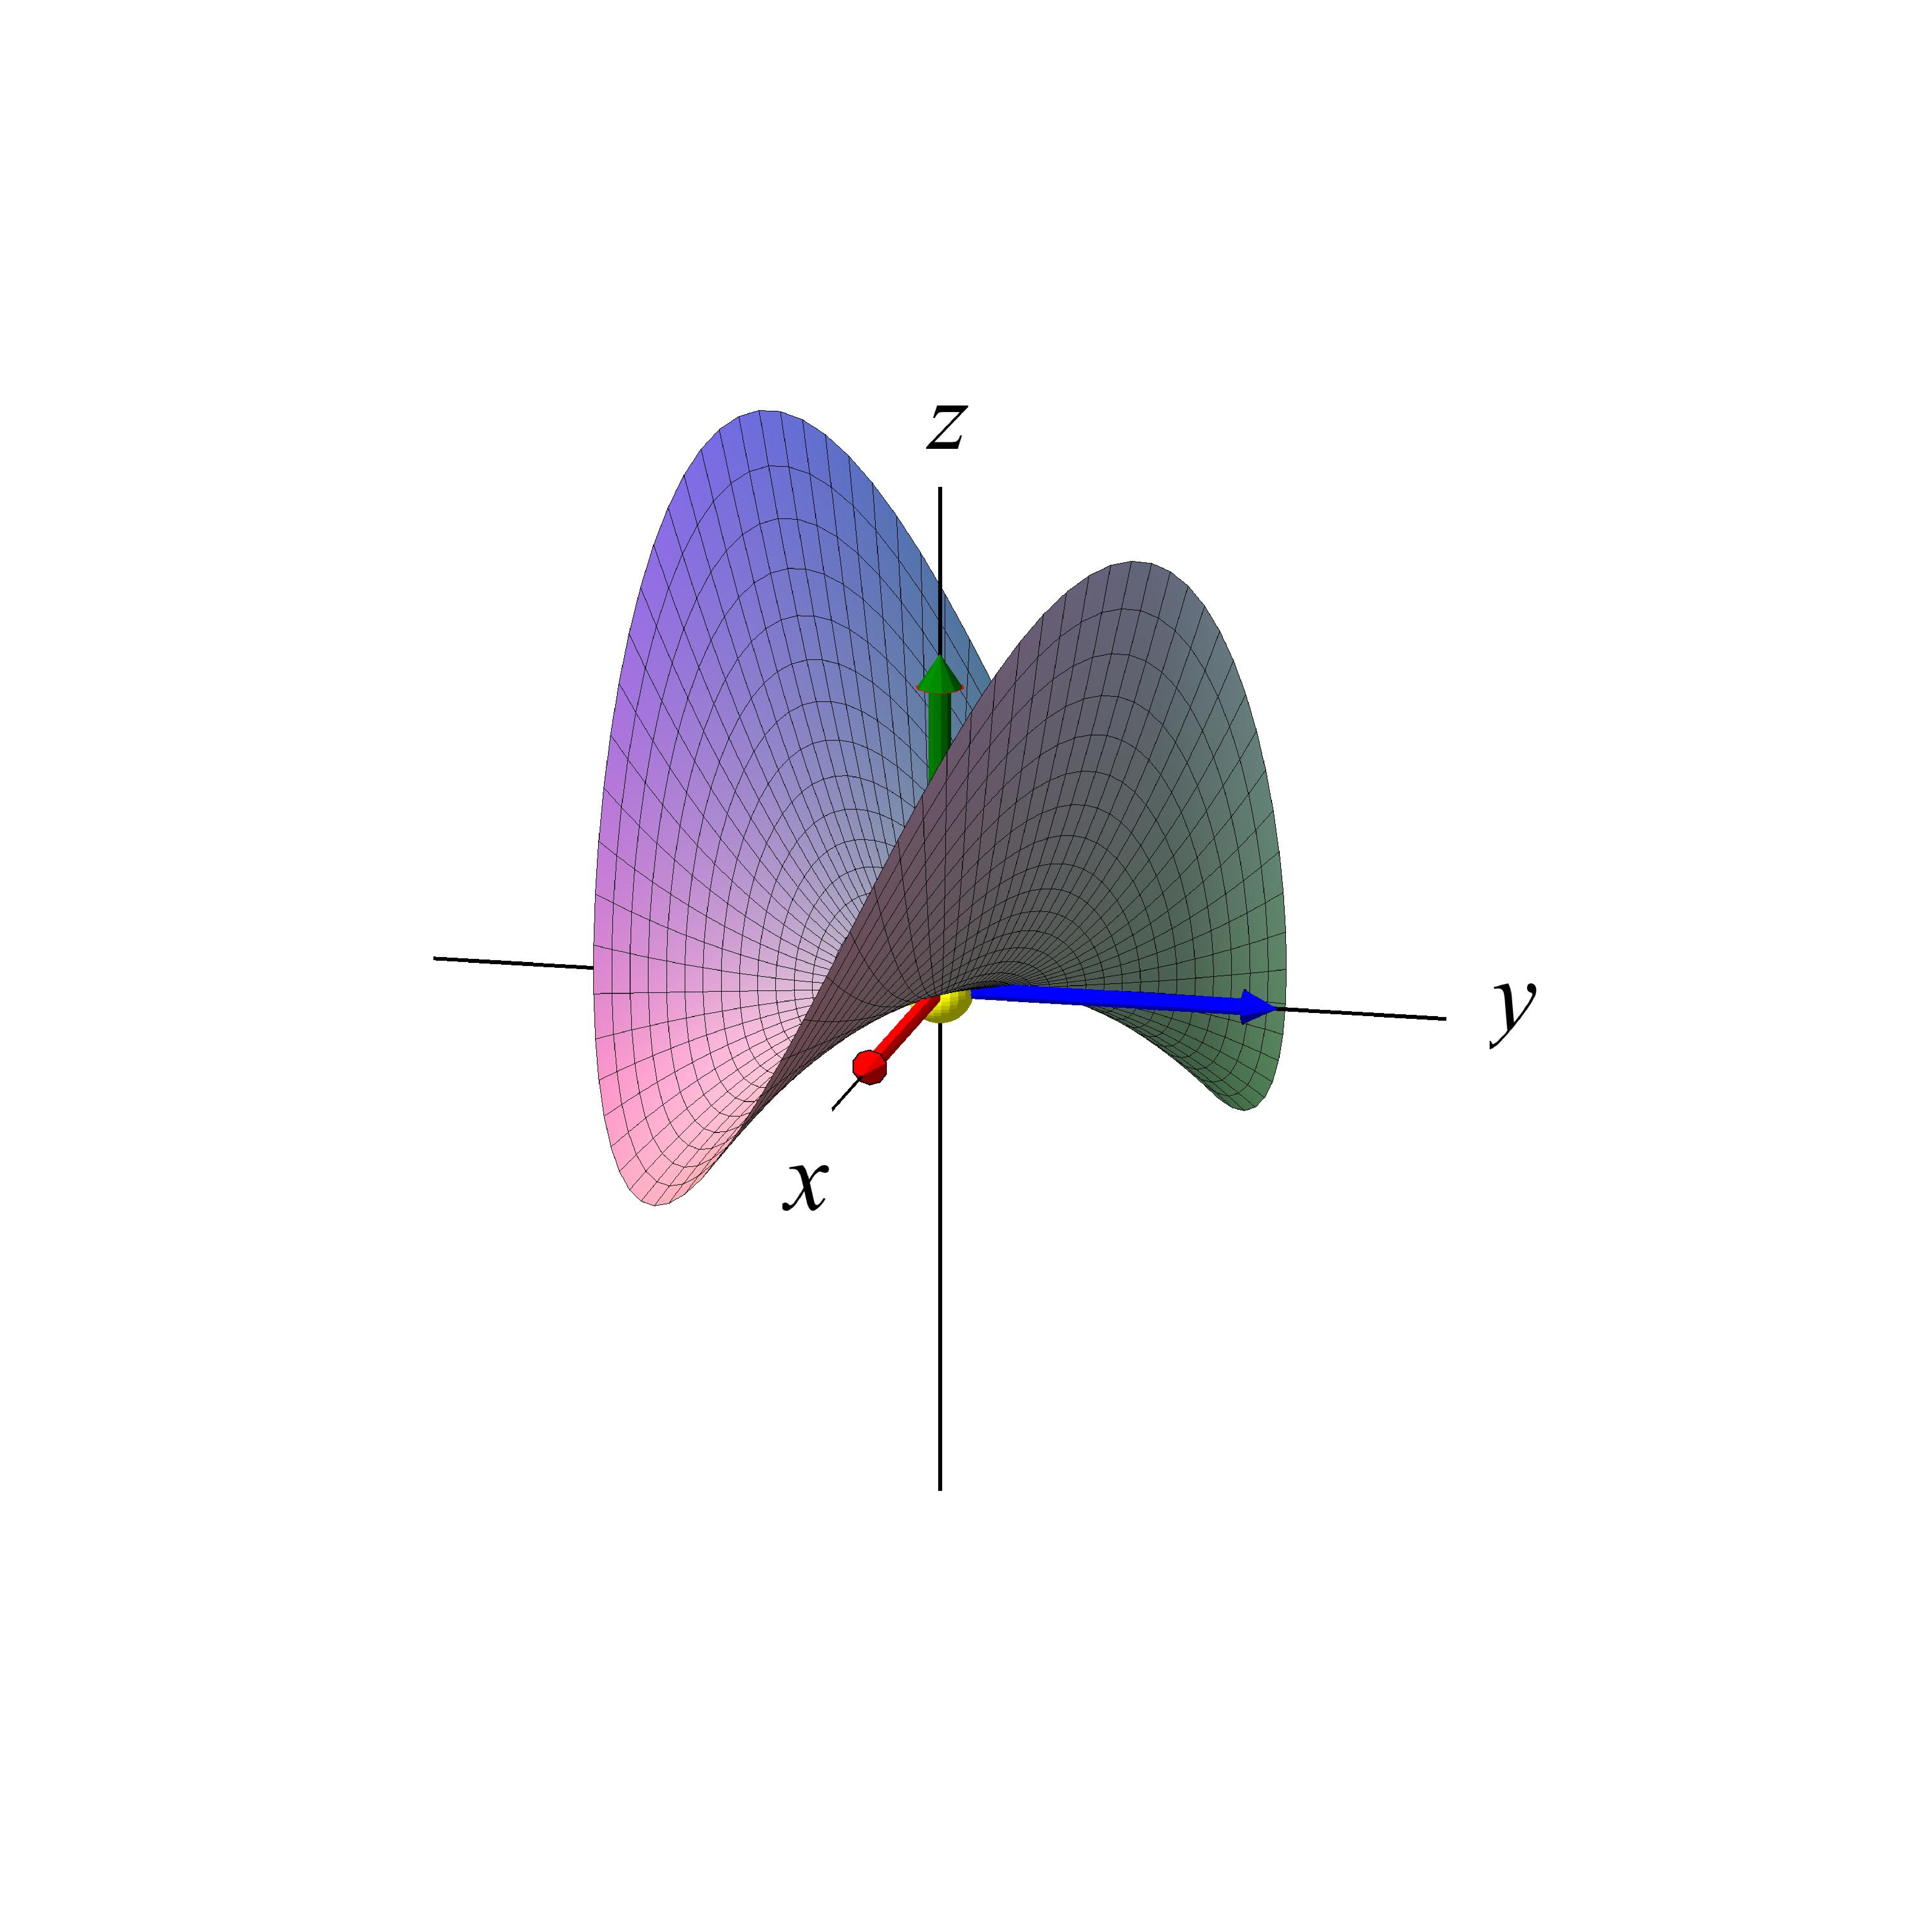
\includegraphics[height=65mm]{plotVar2Fig.pdf}  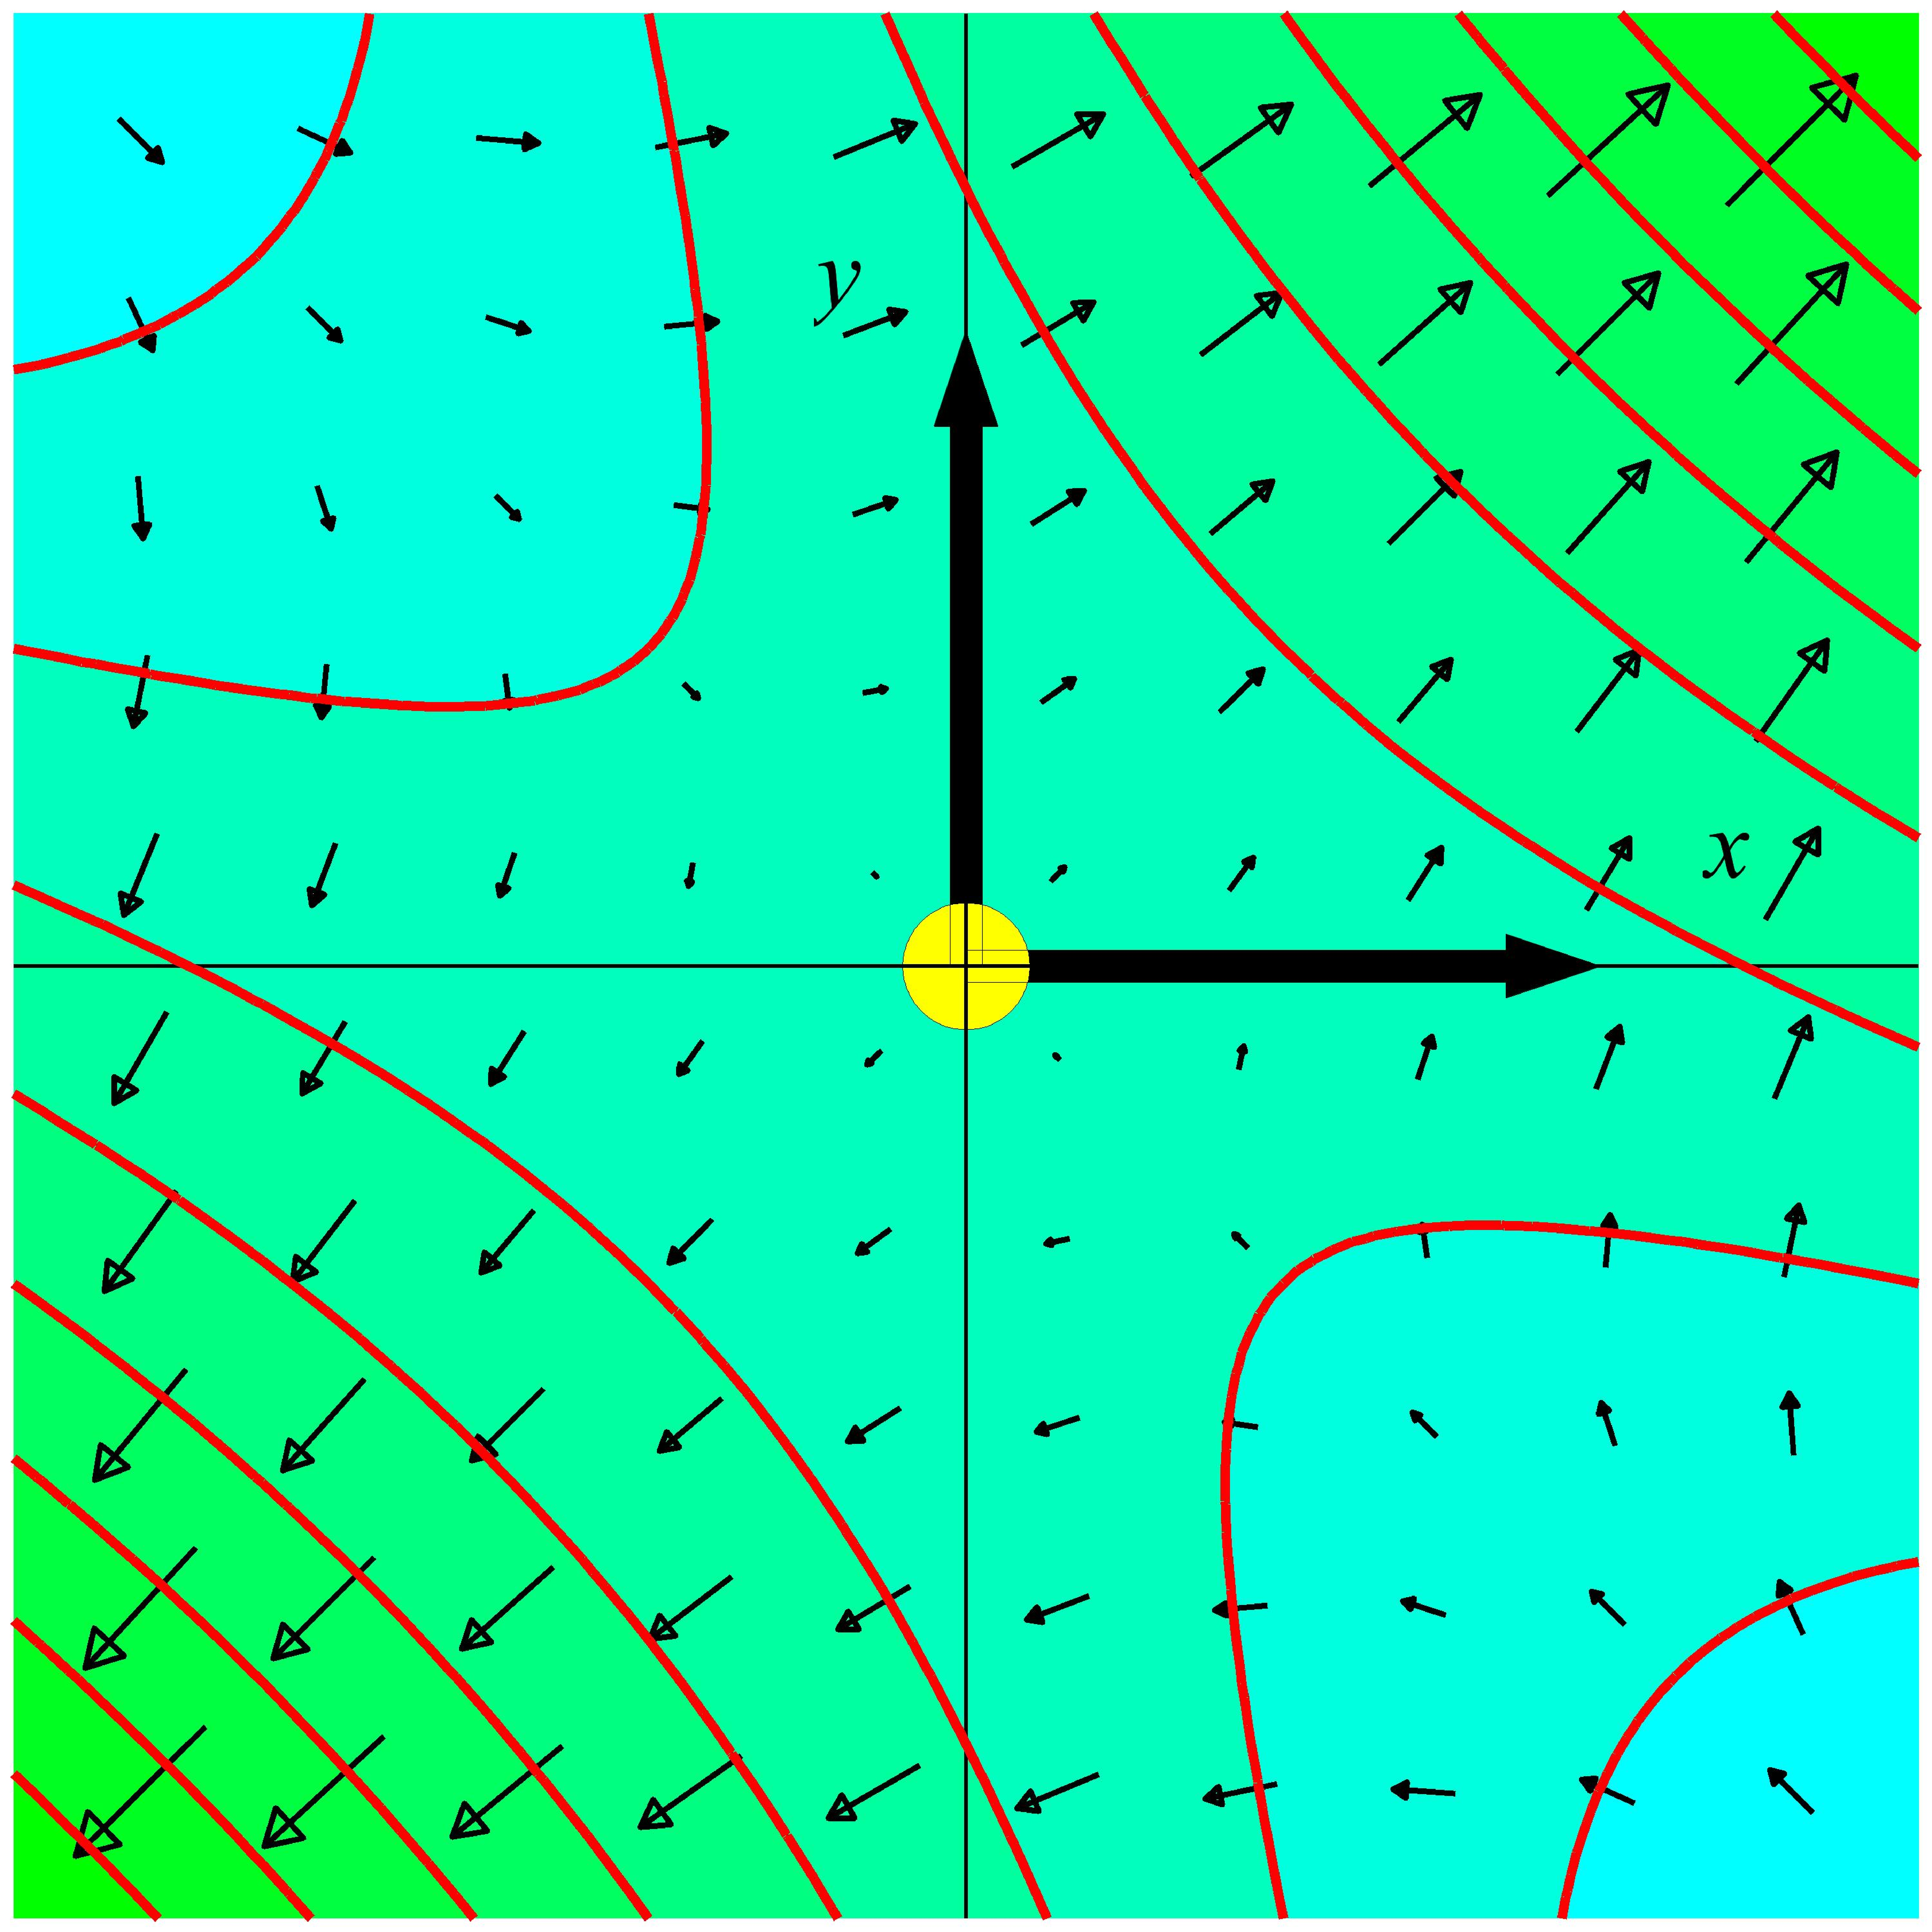
\includegraphics[height=35mm]{plotGrad.pdf} }
\begin{center}
\caption{Grafen for funktionen $f(x,y)= \frac{1}{2}\cdot \left(x^{2} + y^{2} + 4\cdot x \cdot y\right)$ er vist til venstre og funktionens niveaukurver med gradientvektorfelt til højre.} \label{figPosHess}
\end{center}
\end{figure}

\begin{example}[Inspektion af stationært punkt] \label{exampApprox3grad}
Lad funktionen $f(x,y)$ være givet ved
\begin{equation*}
f(x,y) = x^{3} + y^{2} + x\cdot y \quad , \quad \bm{\nabla}f(x,y) = (3\cdot x^{2} + y, x + 2\cdot y) \quad , \quad \mathbf{H}f(x, y) = \left[
                                                                                                  \begin{array}{cc}
                                                                                                    6\cdot x & 1 \\
                                                                                                    1 & 2 \\
                                                                                                  \end{array}
                                                                                                \right] \quad .
\end{equation*}
Så er $(0,0)$ et stationært punkt for $f(x,y)$ og egenværdierne for $\mathbf{H}f(0,0)$ er henholdsvis $\lambda_{1}(x_{0}, y_{0}) = 1 + \sqrt{2} > 0 $ og $\lambda_{2}(x_{0}, y_{0}) = 1 - \sqrt{2} < 0$. Se figur \ref{figPosHess3}. Der er tydeligvis hverken lokalt minimum eller lokalt maksimum i det stationære punkt i overensstemmelse med hjælpesætning\ref{lemmaEkstrema2Var}.
\end{example}


\begin{figure}[ht]
\centerline{ 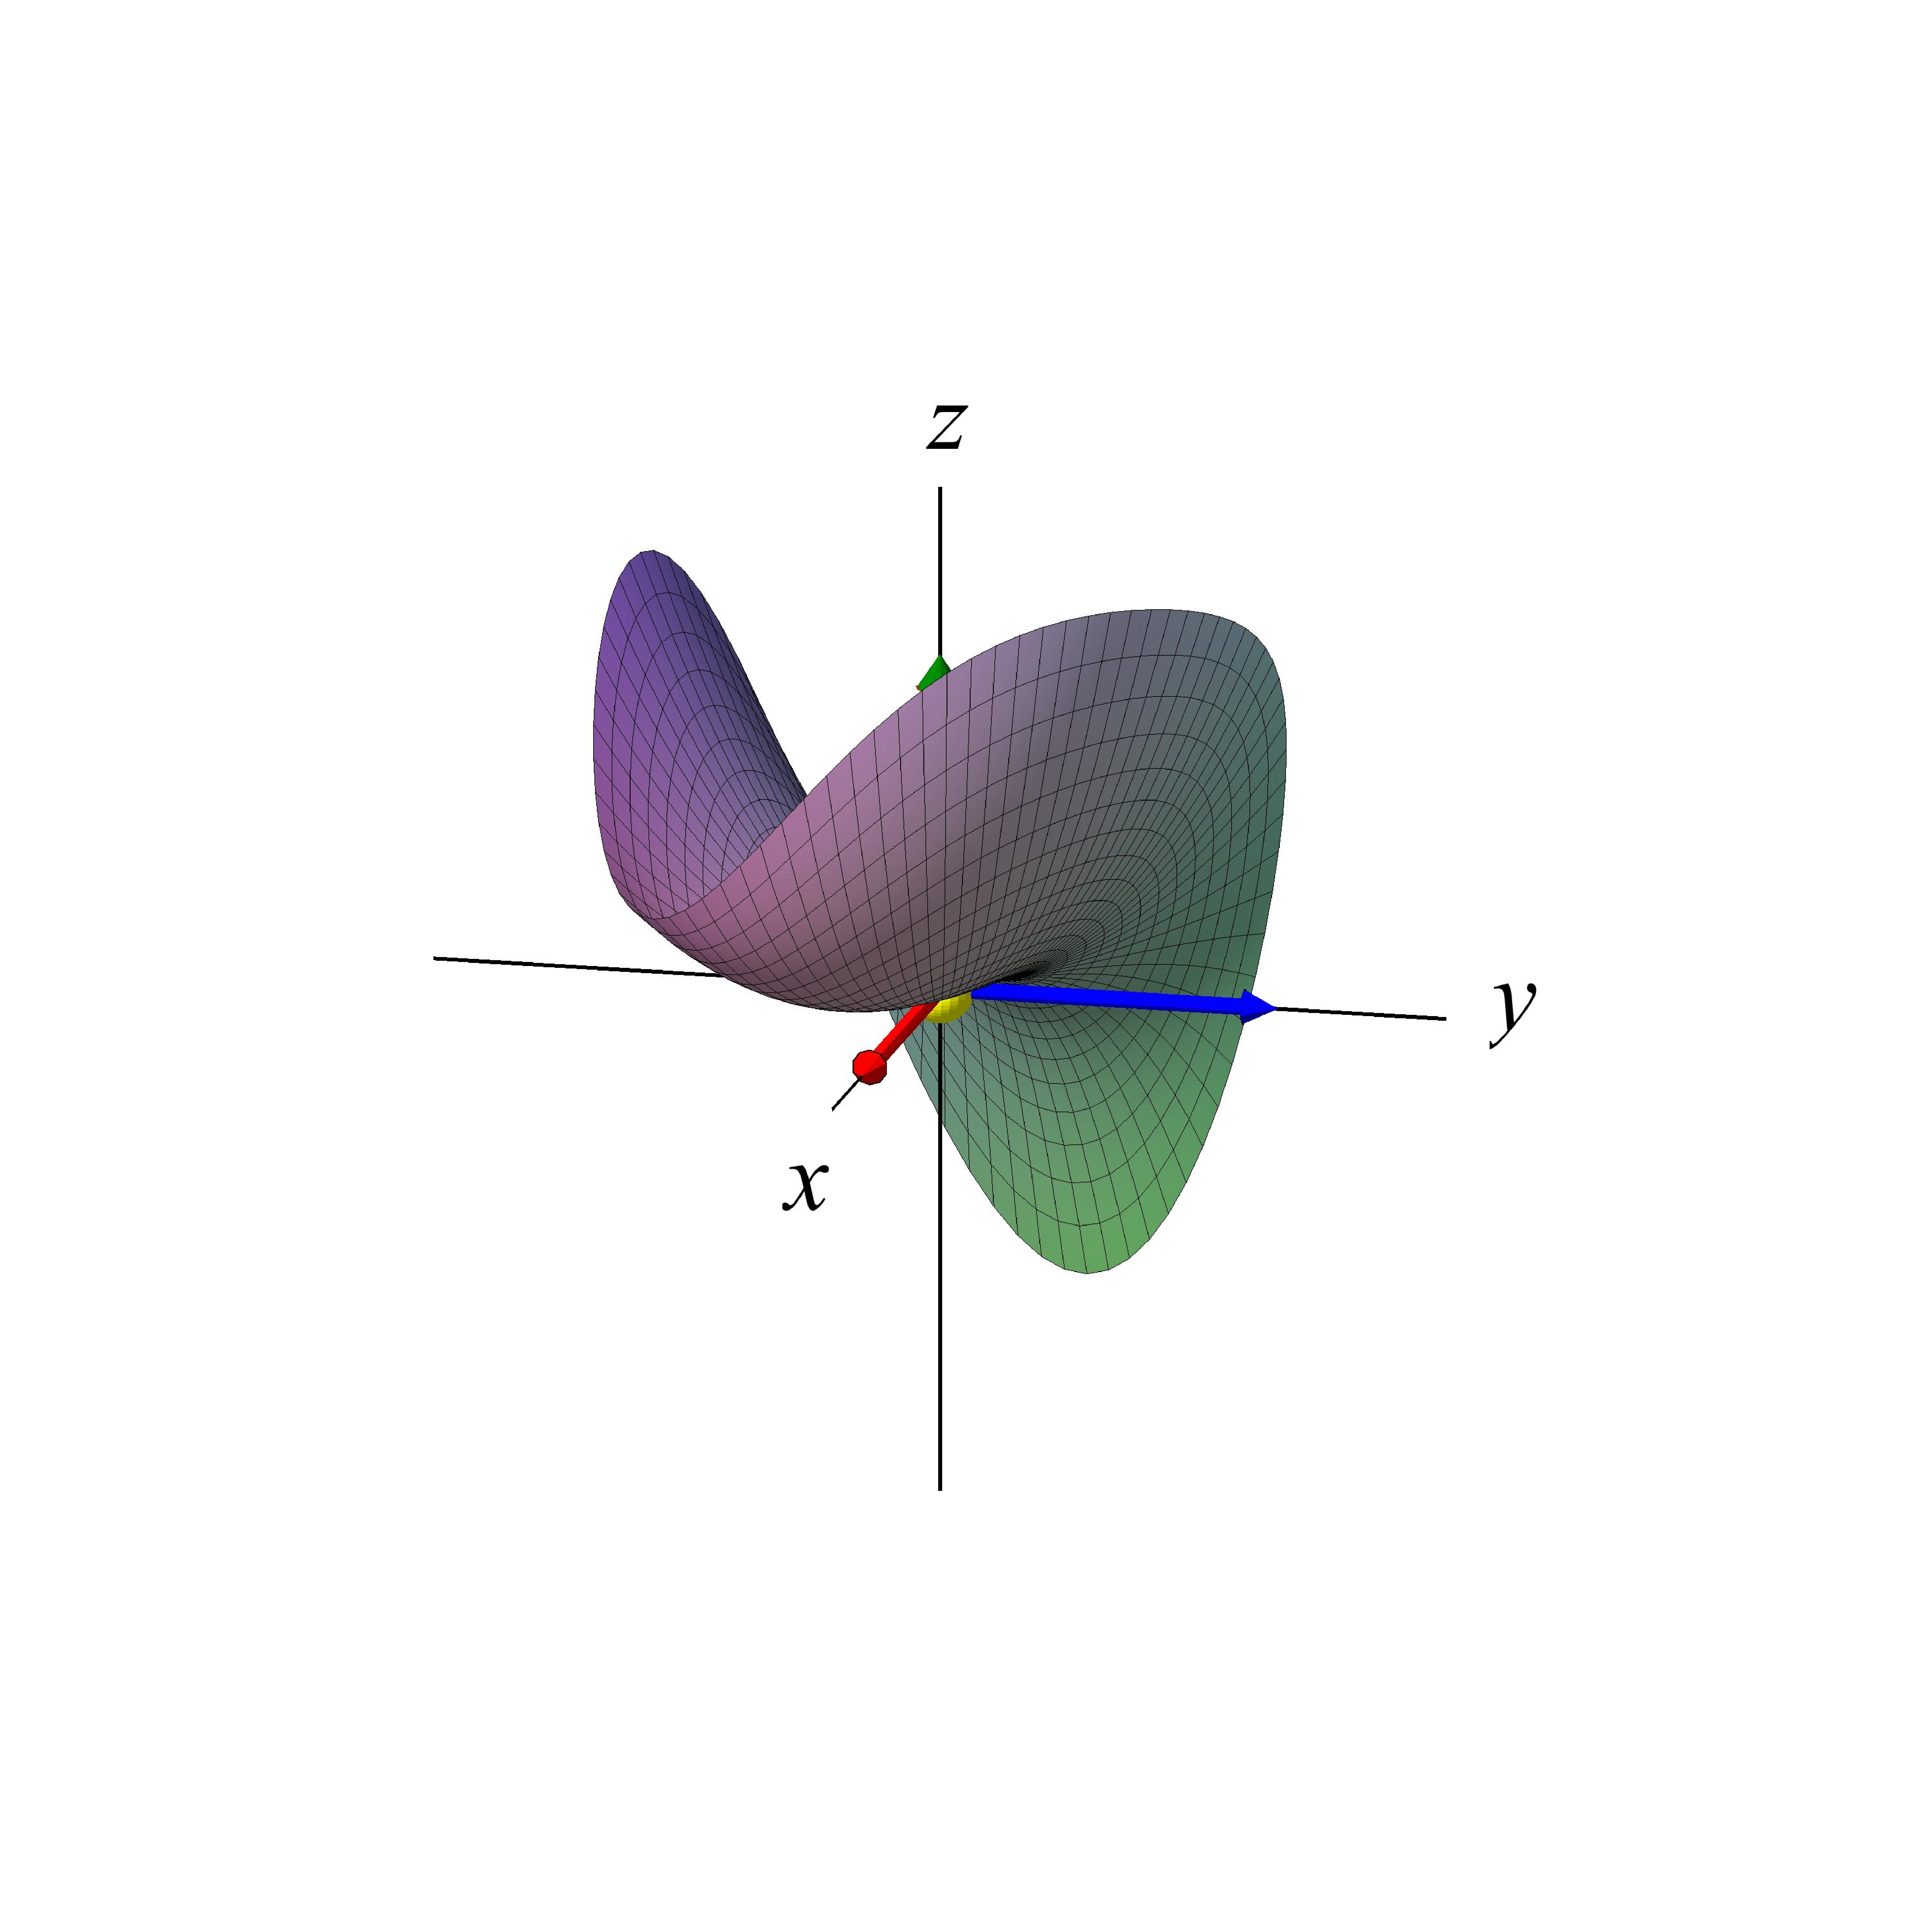
\includegraphics[height=60mm]{plotVar2Fig3.pdf}  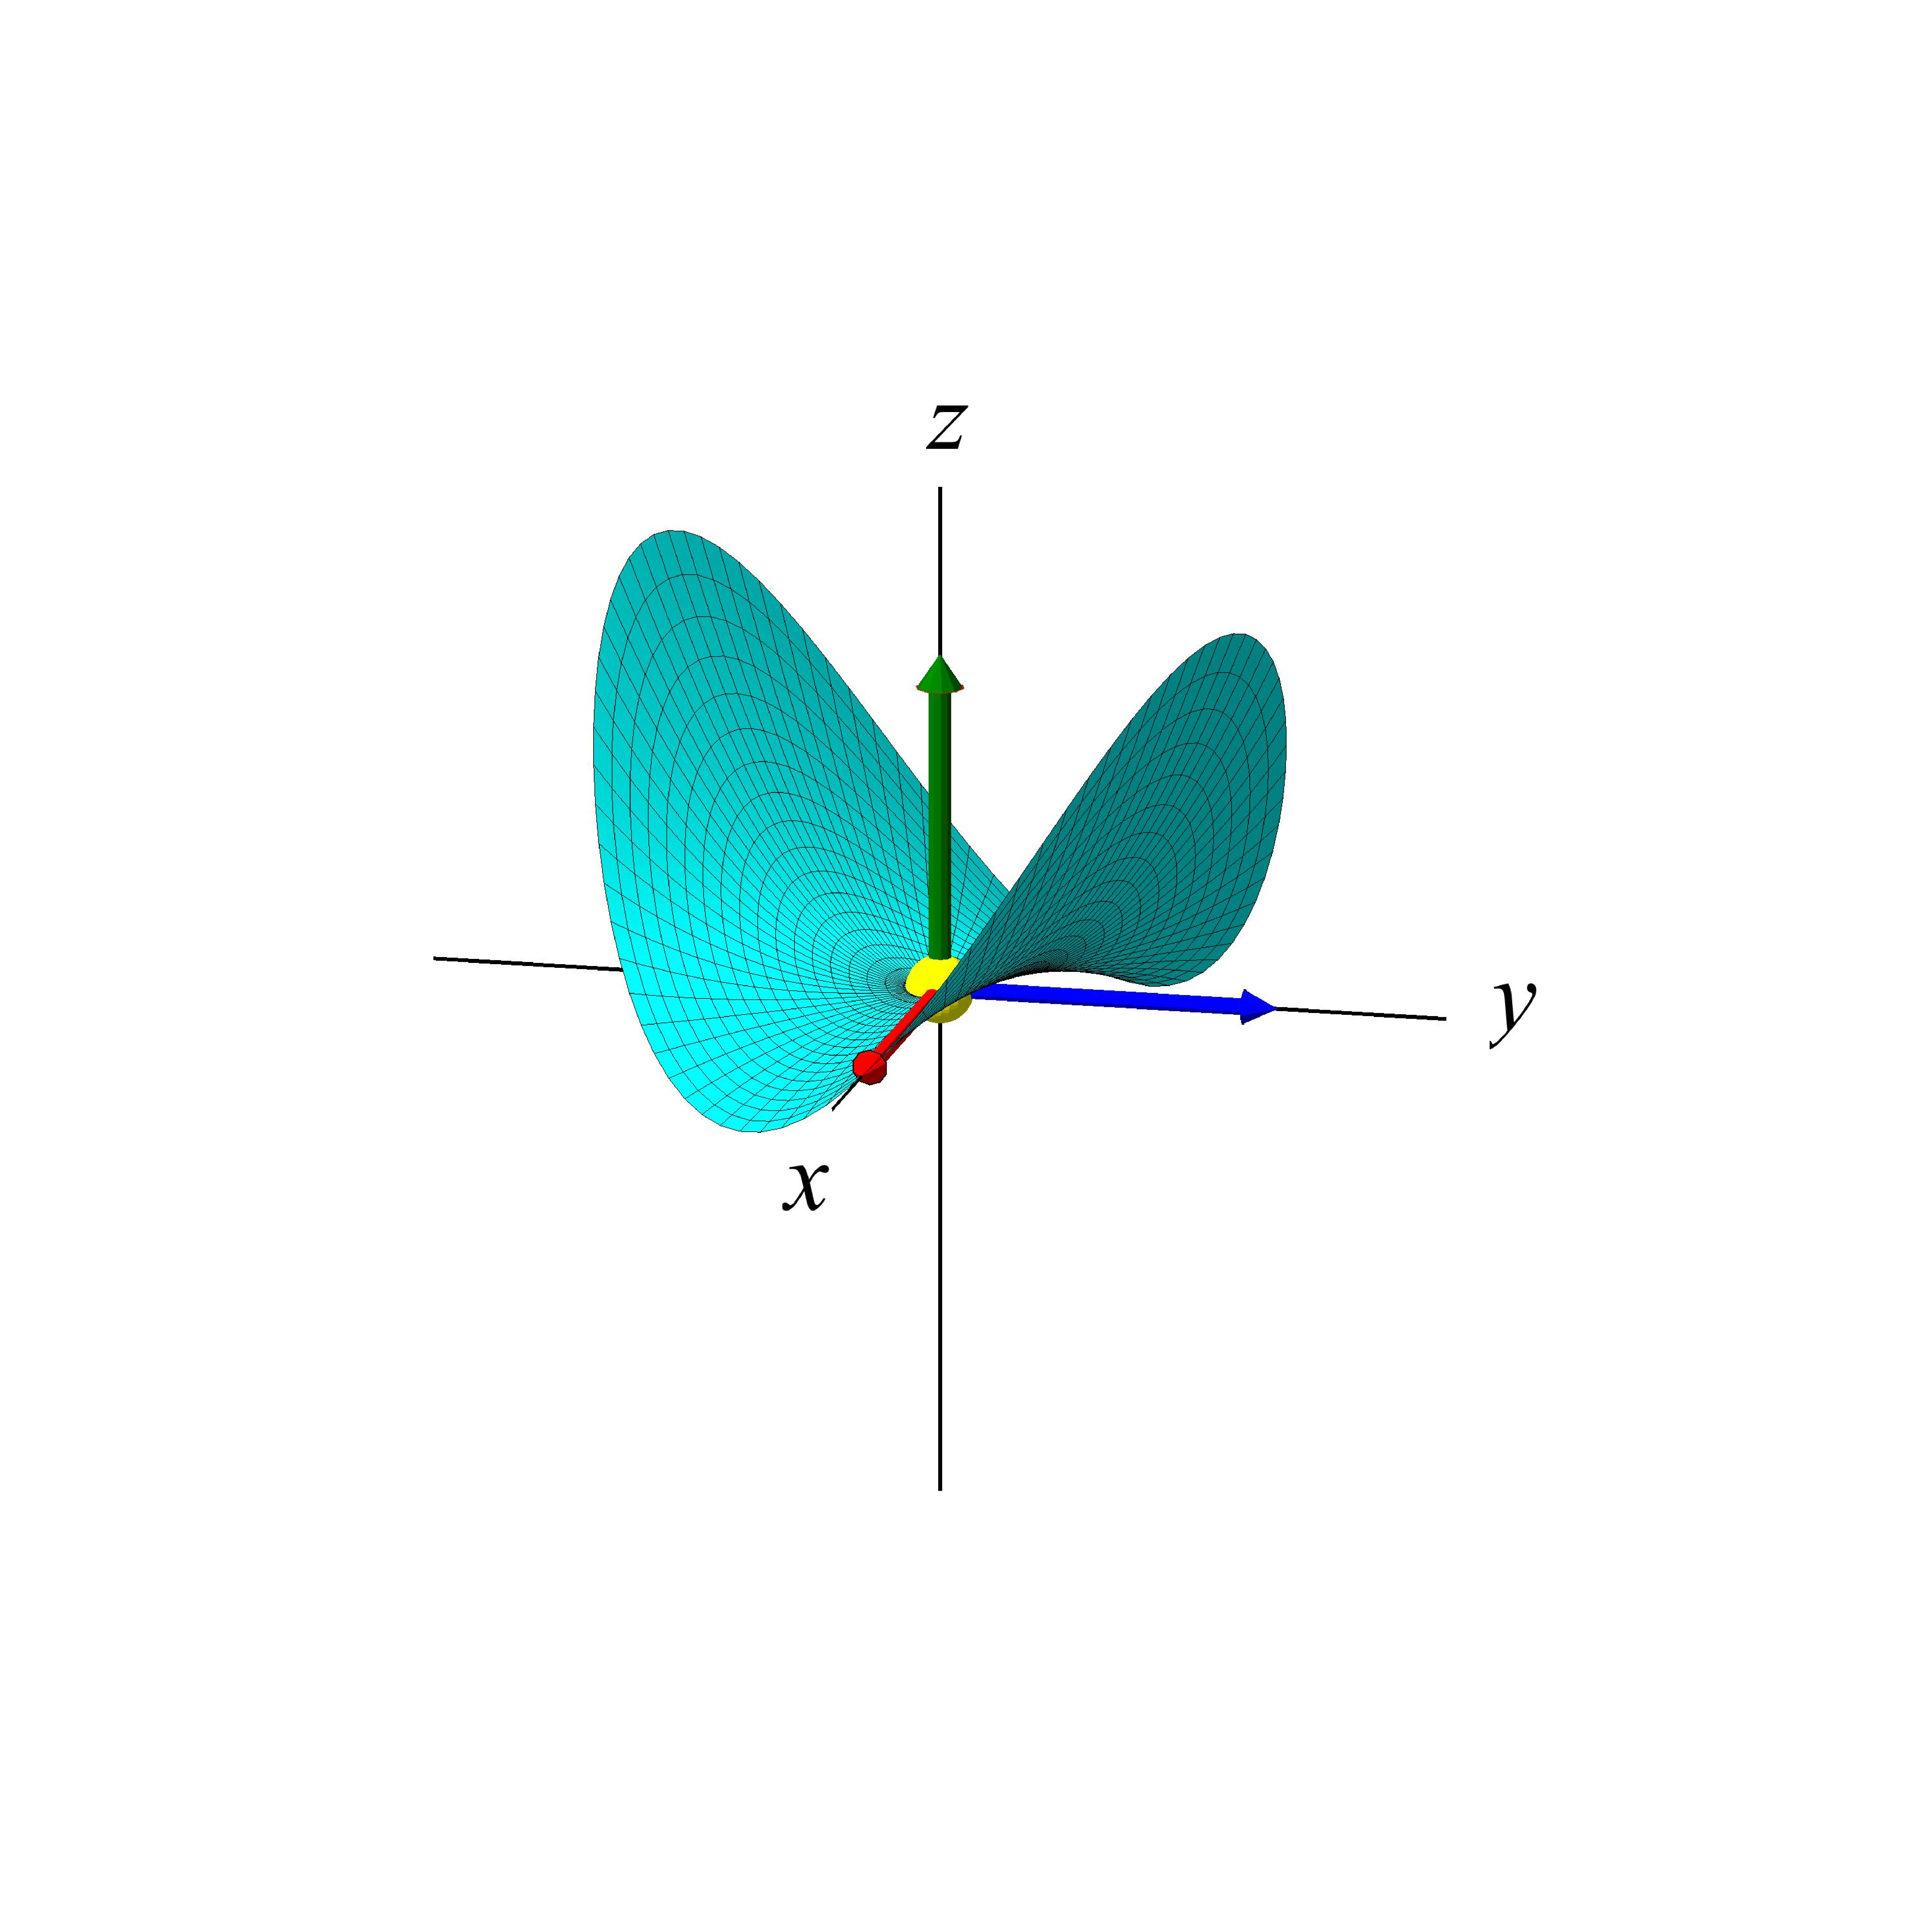
\includegraphics[height=60mm]{plotVar2App3.pdf}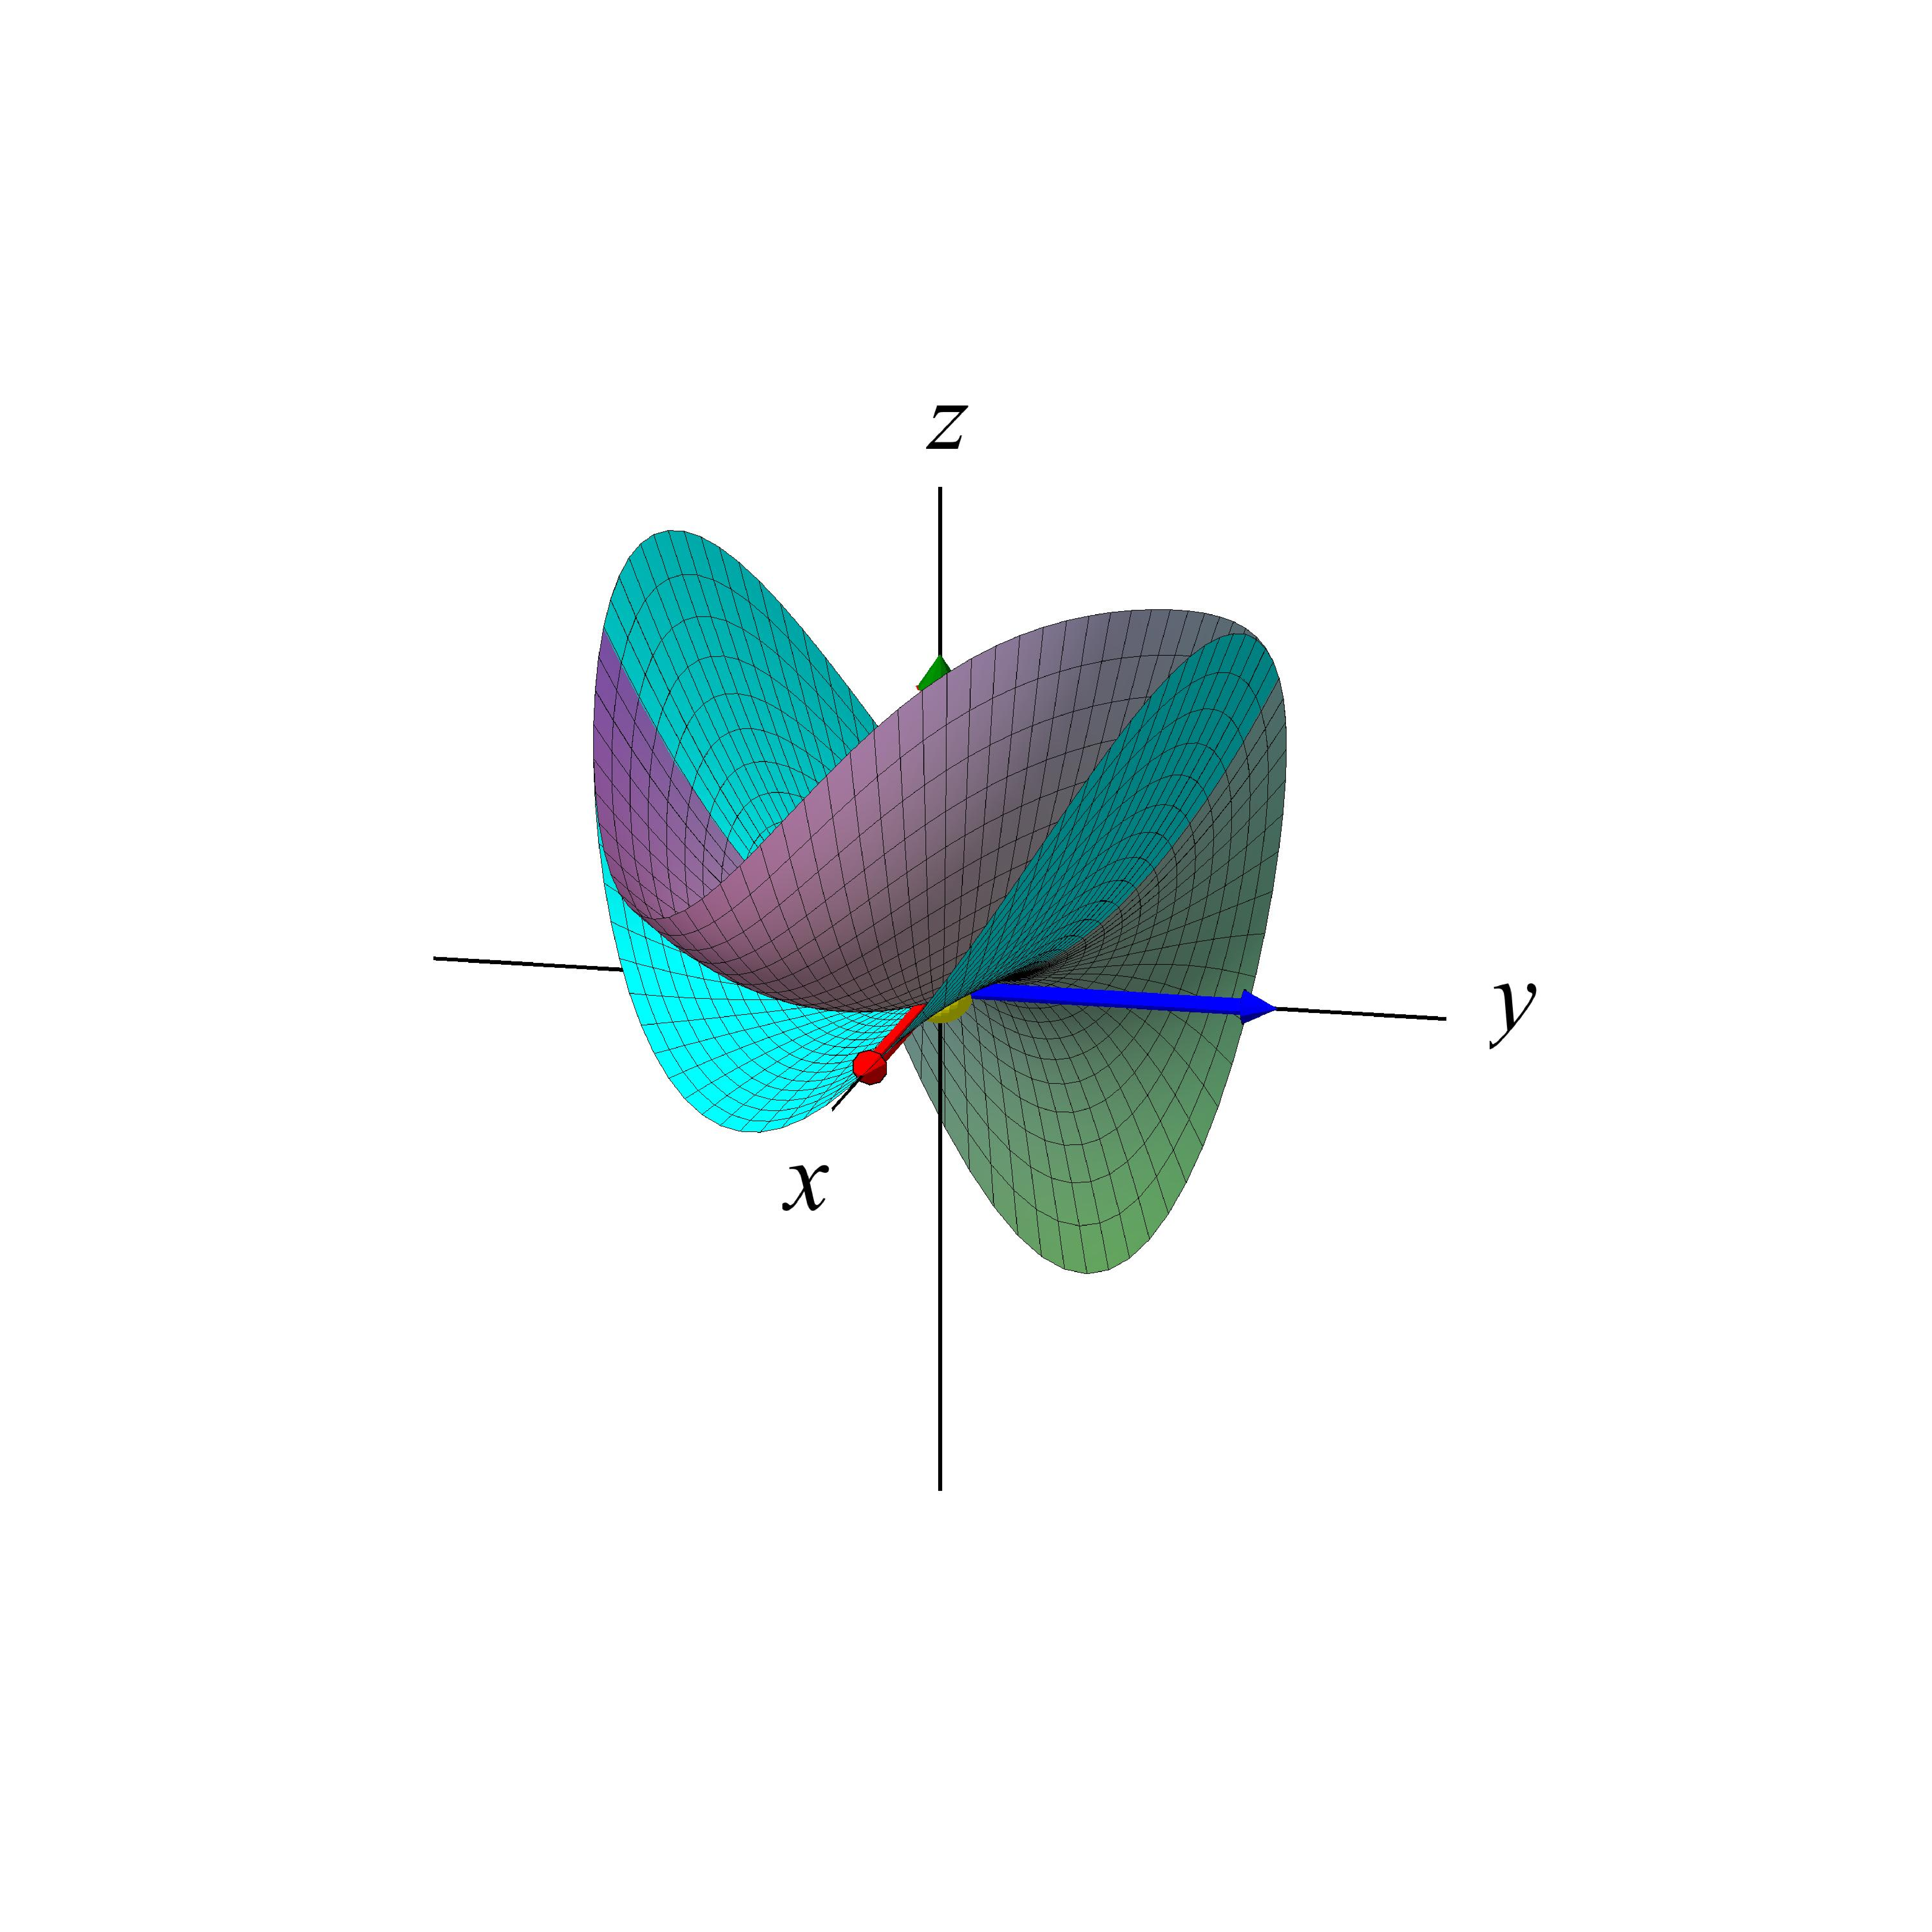
\includegraphics[height=60mm]{plotVar2FigApp3.pdf}  }
\begin{center}
\caption{Grafen for funktionen $f(x,y)= x^{3} + y^{2} + x\cdot y$ er vist til venstre, grafen for det approksimerende andengrads-polynomium med udviklingspunkt $(0,0)$ er vist i midten, begge i samme plot til højre.} \label{figPosHess3}
\end{center}
\end{figure}

\begin{figure}[ht]
\centerline{ 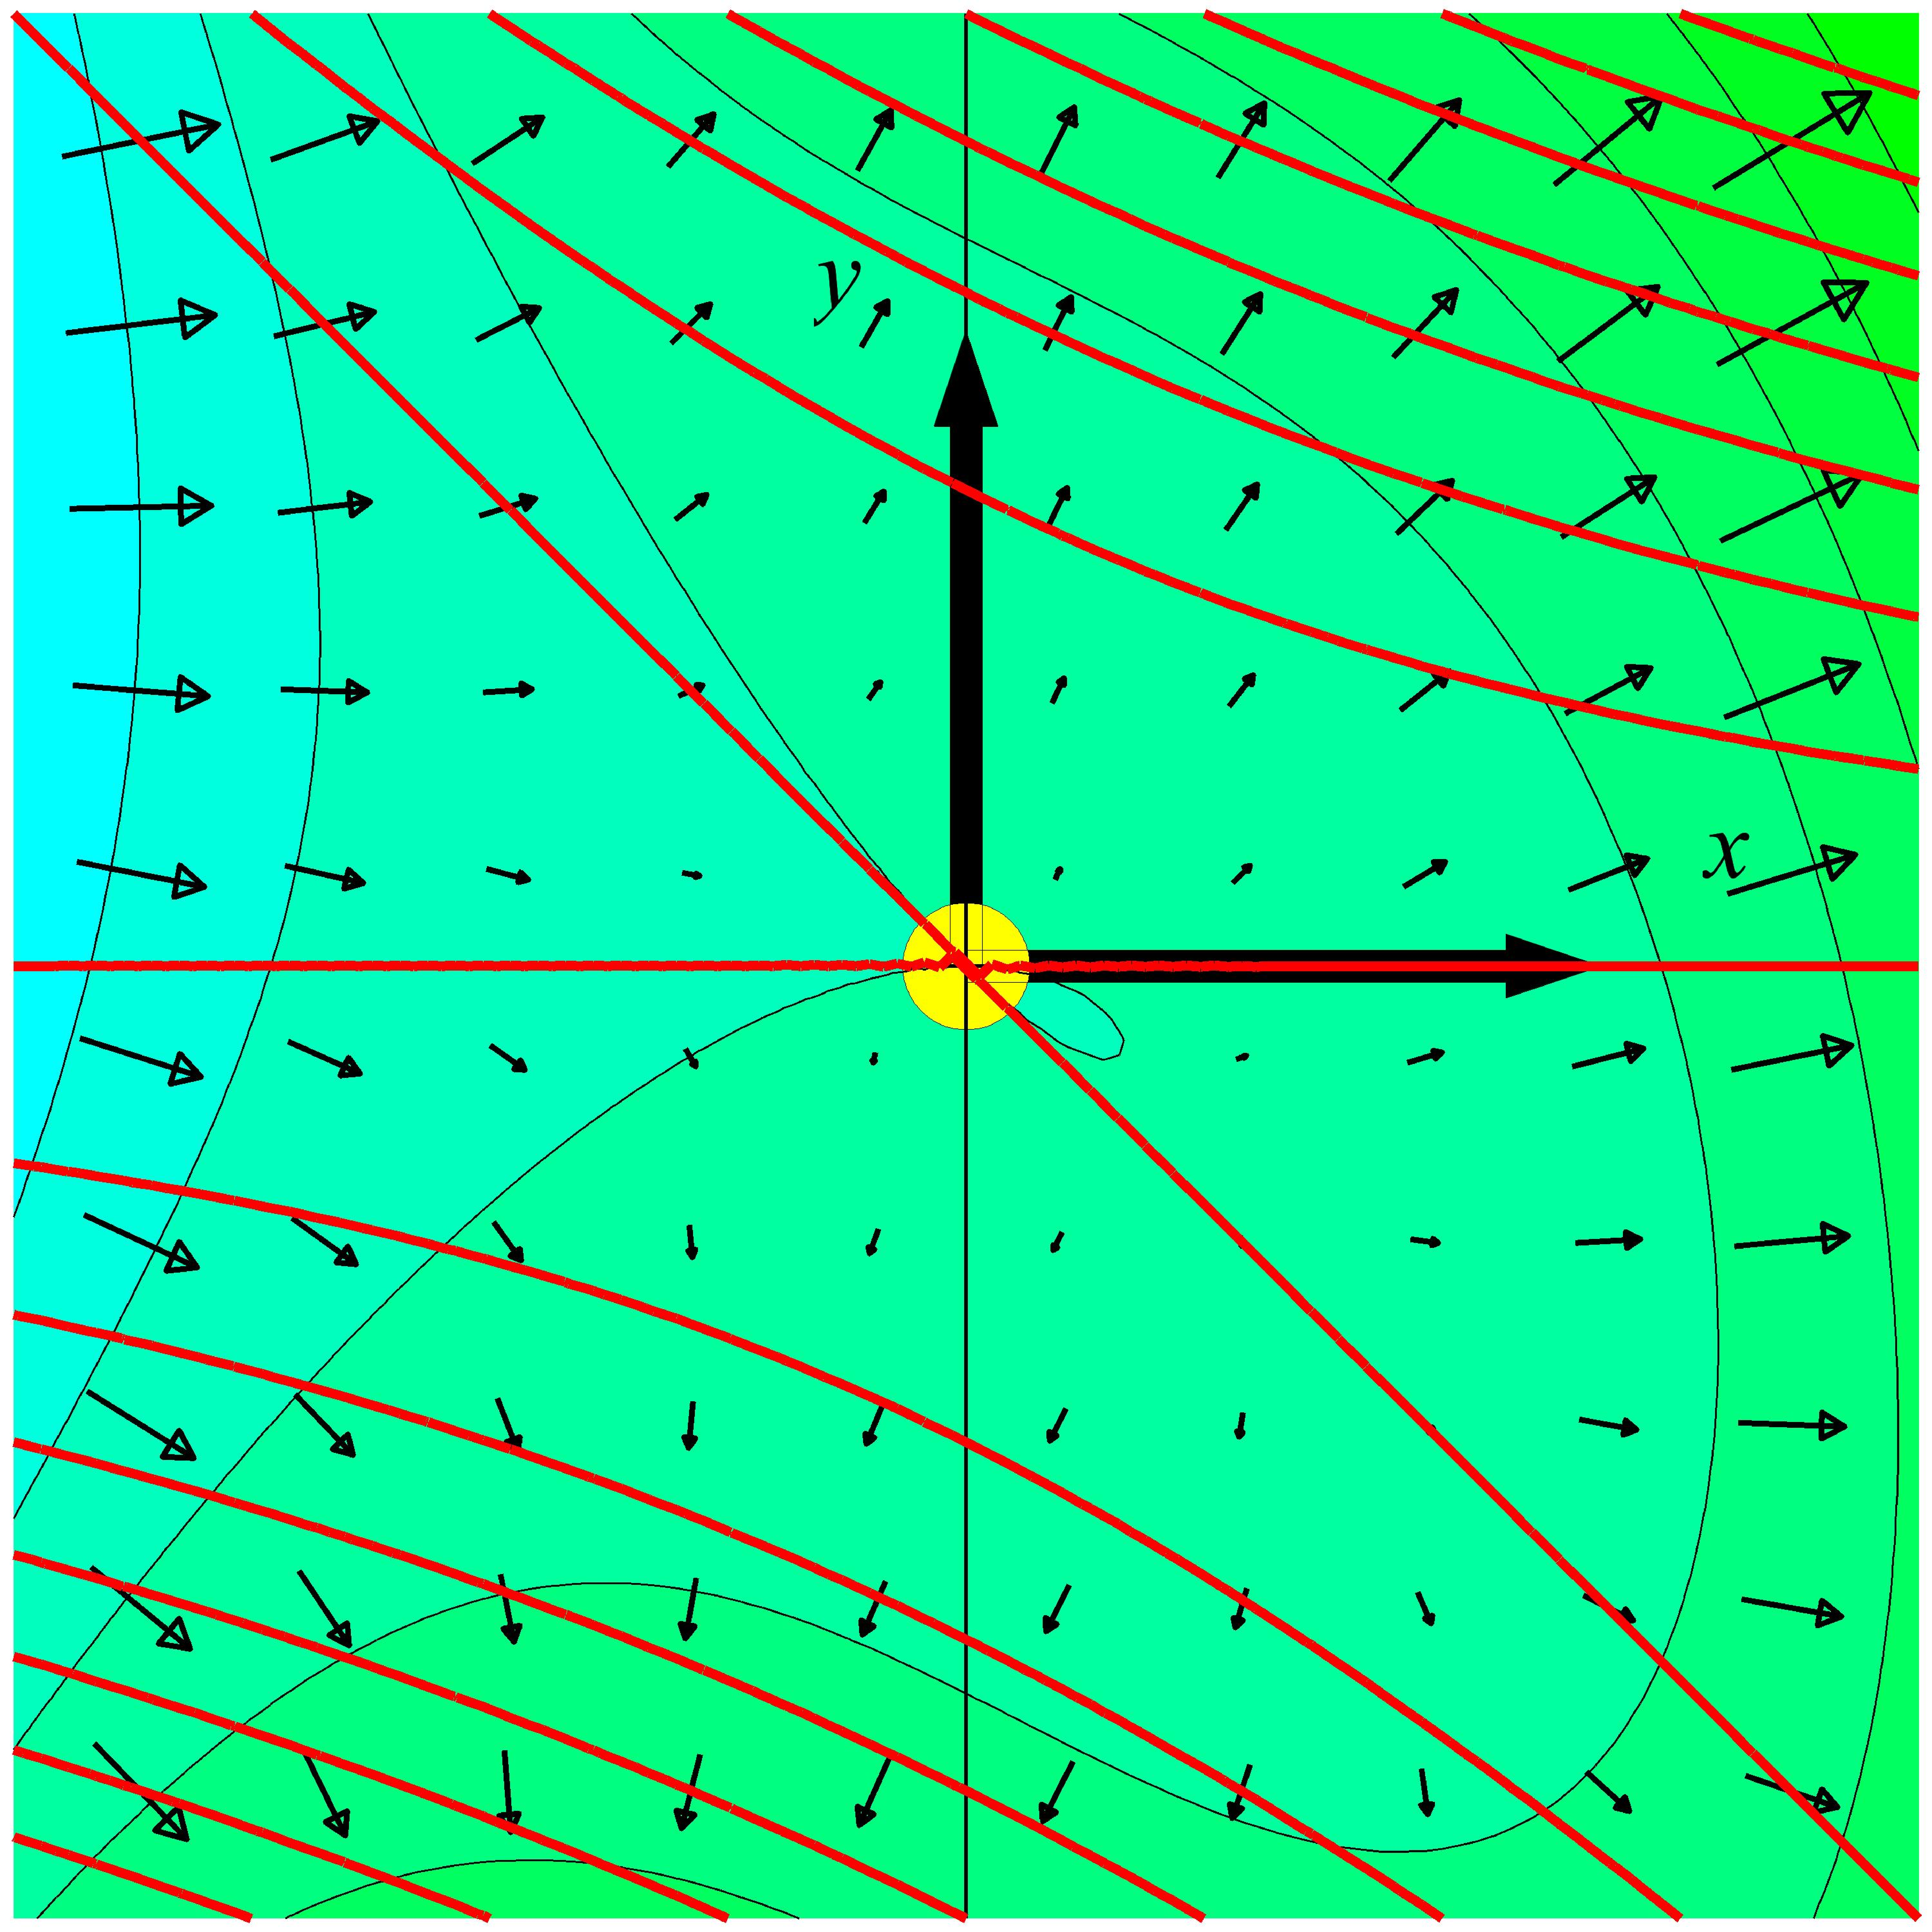
\includegraphics[height=55mm]{plotGrad3.pdf}}
\begin{center}
\caption{Niveaukurver (sorte) og gradientvektorfeltet for funktionen $f(x,y)= x^{3} + y^{2} + x\cdot y$ sammen med nogle niveaukurver (røde) for det approksimerende an\-dengrads\-polynomium for $f(x,y)$ omkring det stationære punkt $(x_{0}, y_{0}) = (0,0)$.} \label{figPosHessNiv3}
\end{center}
\end{figure}



\begin{exercise}
Funktionen $f(x,y) = x^{3} + y^{2} + x\cdot y$ som vi undersøgte i eksempel \ref{exampApprox3grad} har også et stationært punkt i $(x_{0}, y_{0}) = (1/12\, , \, -1/24)$. Undersøg, om dette stationære punkt er et lokalt maksimum eller et lokalt minimum eller ingen af delene for $f(x,y)$.
\end{exercise}


\begin{example}[Inspektion af stationært punkt] \label{exampStatInspec1}
Lad funktionen $f(x,y)$ være givet med følgende data i $\mathbb{R}^{2}$:
\begin{equation}
\begin{aligned}
f(x,y) &= \sin(x)\cdot\cos(x\cdot y) \quad , \\
\bm{\nabla}f(x,y) &= \left(\cos(x)\cos(x\cdot y) - y\cdot \sin(x)\cdot\sin(x\cdot y), -x \cdot \sin(x)\cdot \sin(x \cdot y)  \right) \quad .
\end{aligned}
\end{equation}
Så er $(x_{0}, y_{0}) = (\pi/2, 0)$ et stationært punkt for $f(x,y)$ og i det punkt har vi
\begin{equation}
\mathbf{H}f(\pi/2, 0) = \left[
                                                                           \begin{array}{cc}
                                                                             -1 & 0 \\
                                                                             0 & -\pi^{2}/4\\
                                                                           \end{array}
                                                                         \right]
\end{equation}
I det stationære punkt har Hesse-matricen således egenværdierne $-1$ og $-\pi^{2}/4$. Vi konklu\-derer, at det stationære punkt er et egentligt lokalt maksimumpunkt for $f(x,y)$ i over\-ens\-stem\-mel\-se med inspektion af figur \ref{figStatInspec1} -- og i overensstemmelse med hjælpesætning \ref{lemmaEkstrema2Var}.
Det approksimerende andengradspolynomium for $f(x,y)$ med udviklingspunkt i det stationære punkt $(x_{0}, y_{0})= (\pi/2, 0)$ er:
\begin{equation}
\begin{aligned}
P_{2, (\pi/2, 0)}(x,y) &= 1 - \frac{1}{2} \left( x - \frac{\pi}{2} \right)^2 - \frac{1}{2} \cdot \frac{\pi^{2}}{4} \cdot y^2 \\
&= \left(1 - \frac{\pi^{2}}{8}\right) + \frac{\pi}{2}\cdot x - \frac{1}{2}\cdot x^{2}  - \frac{\pi^{2}}{8} \cdot y^{2} \quad.
\end{aligned}
\end{equation}
\end{example}


\begin{figure}[ht]
\centerline{ 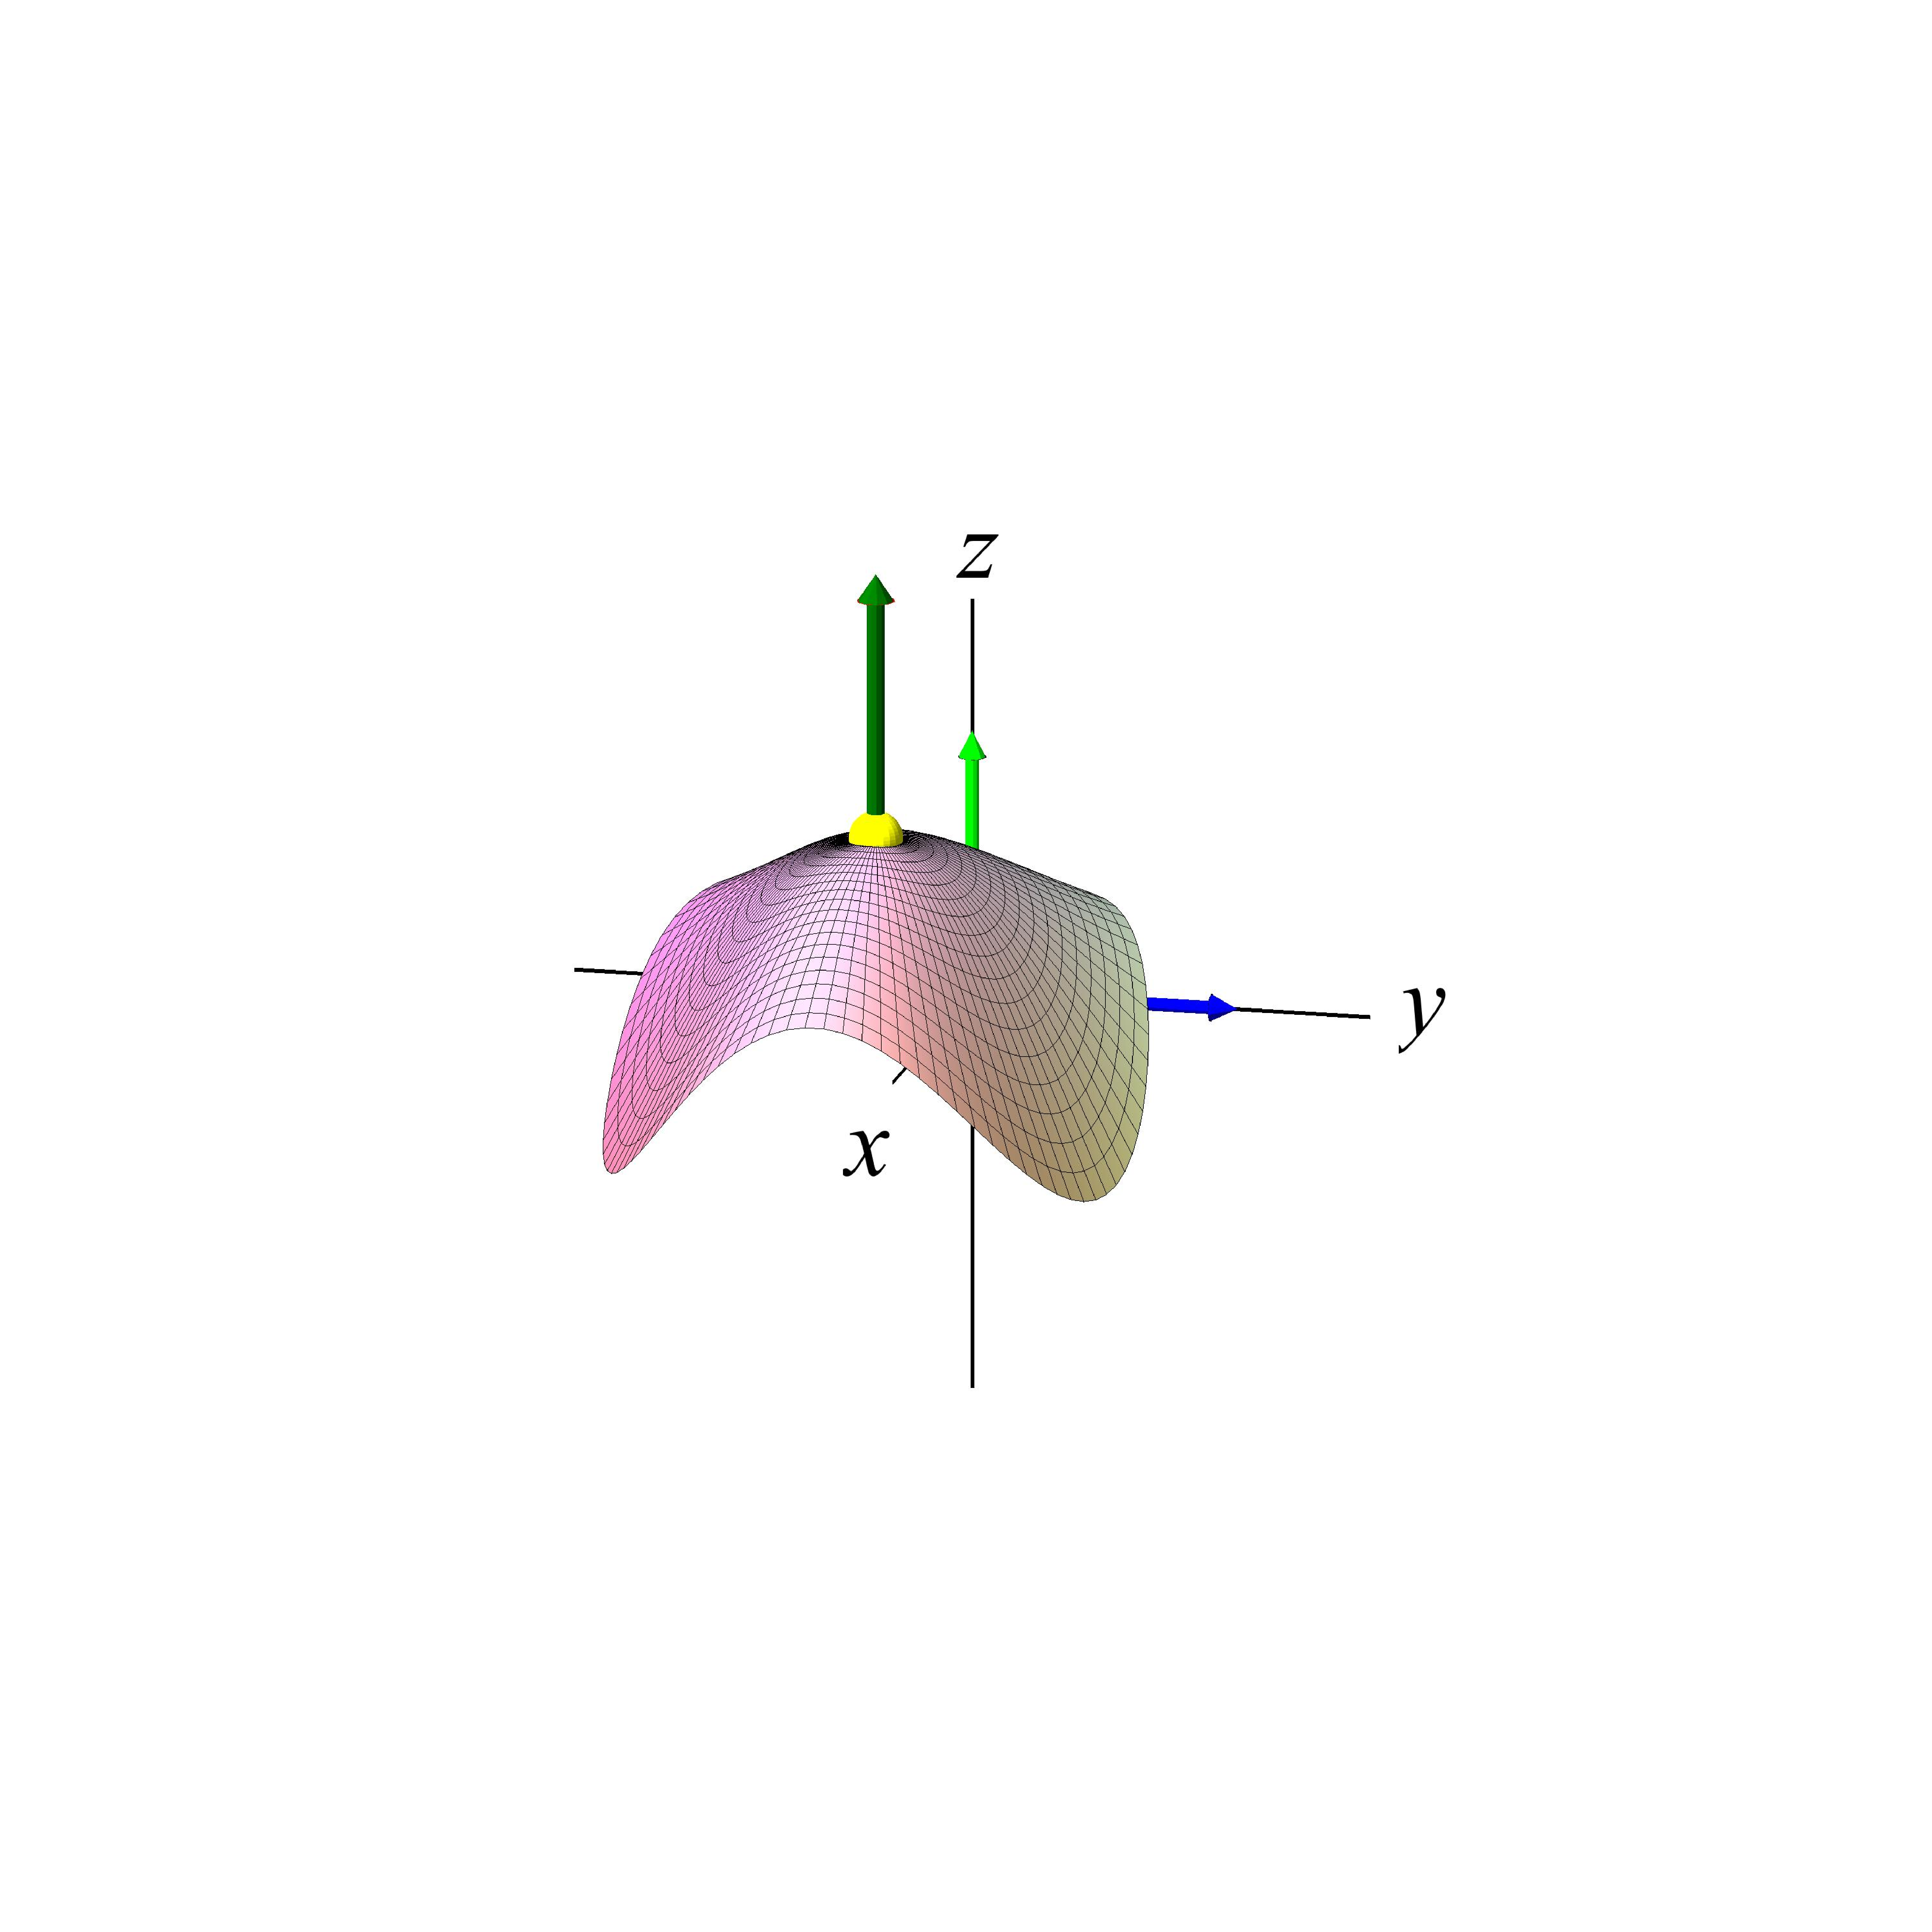
\includegraphics[height=55mm]{plotVar2Fig2.pdf} 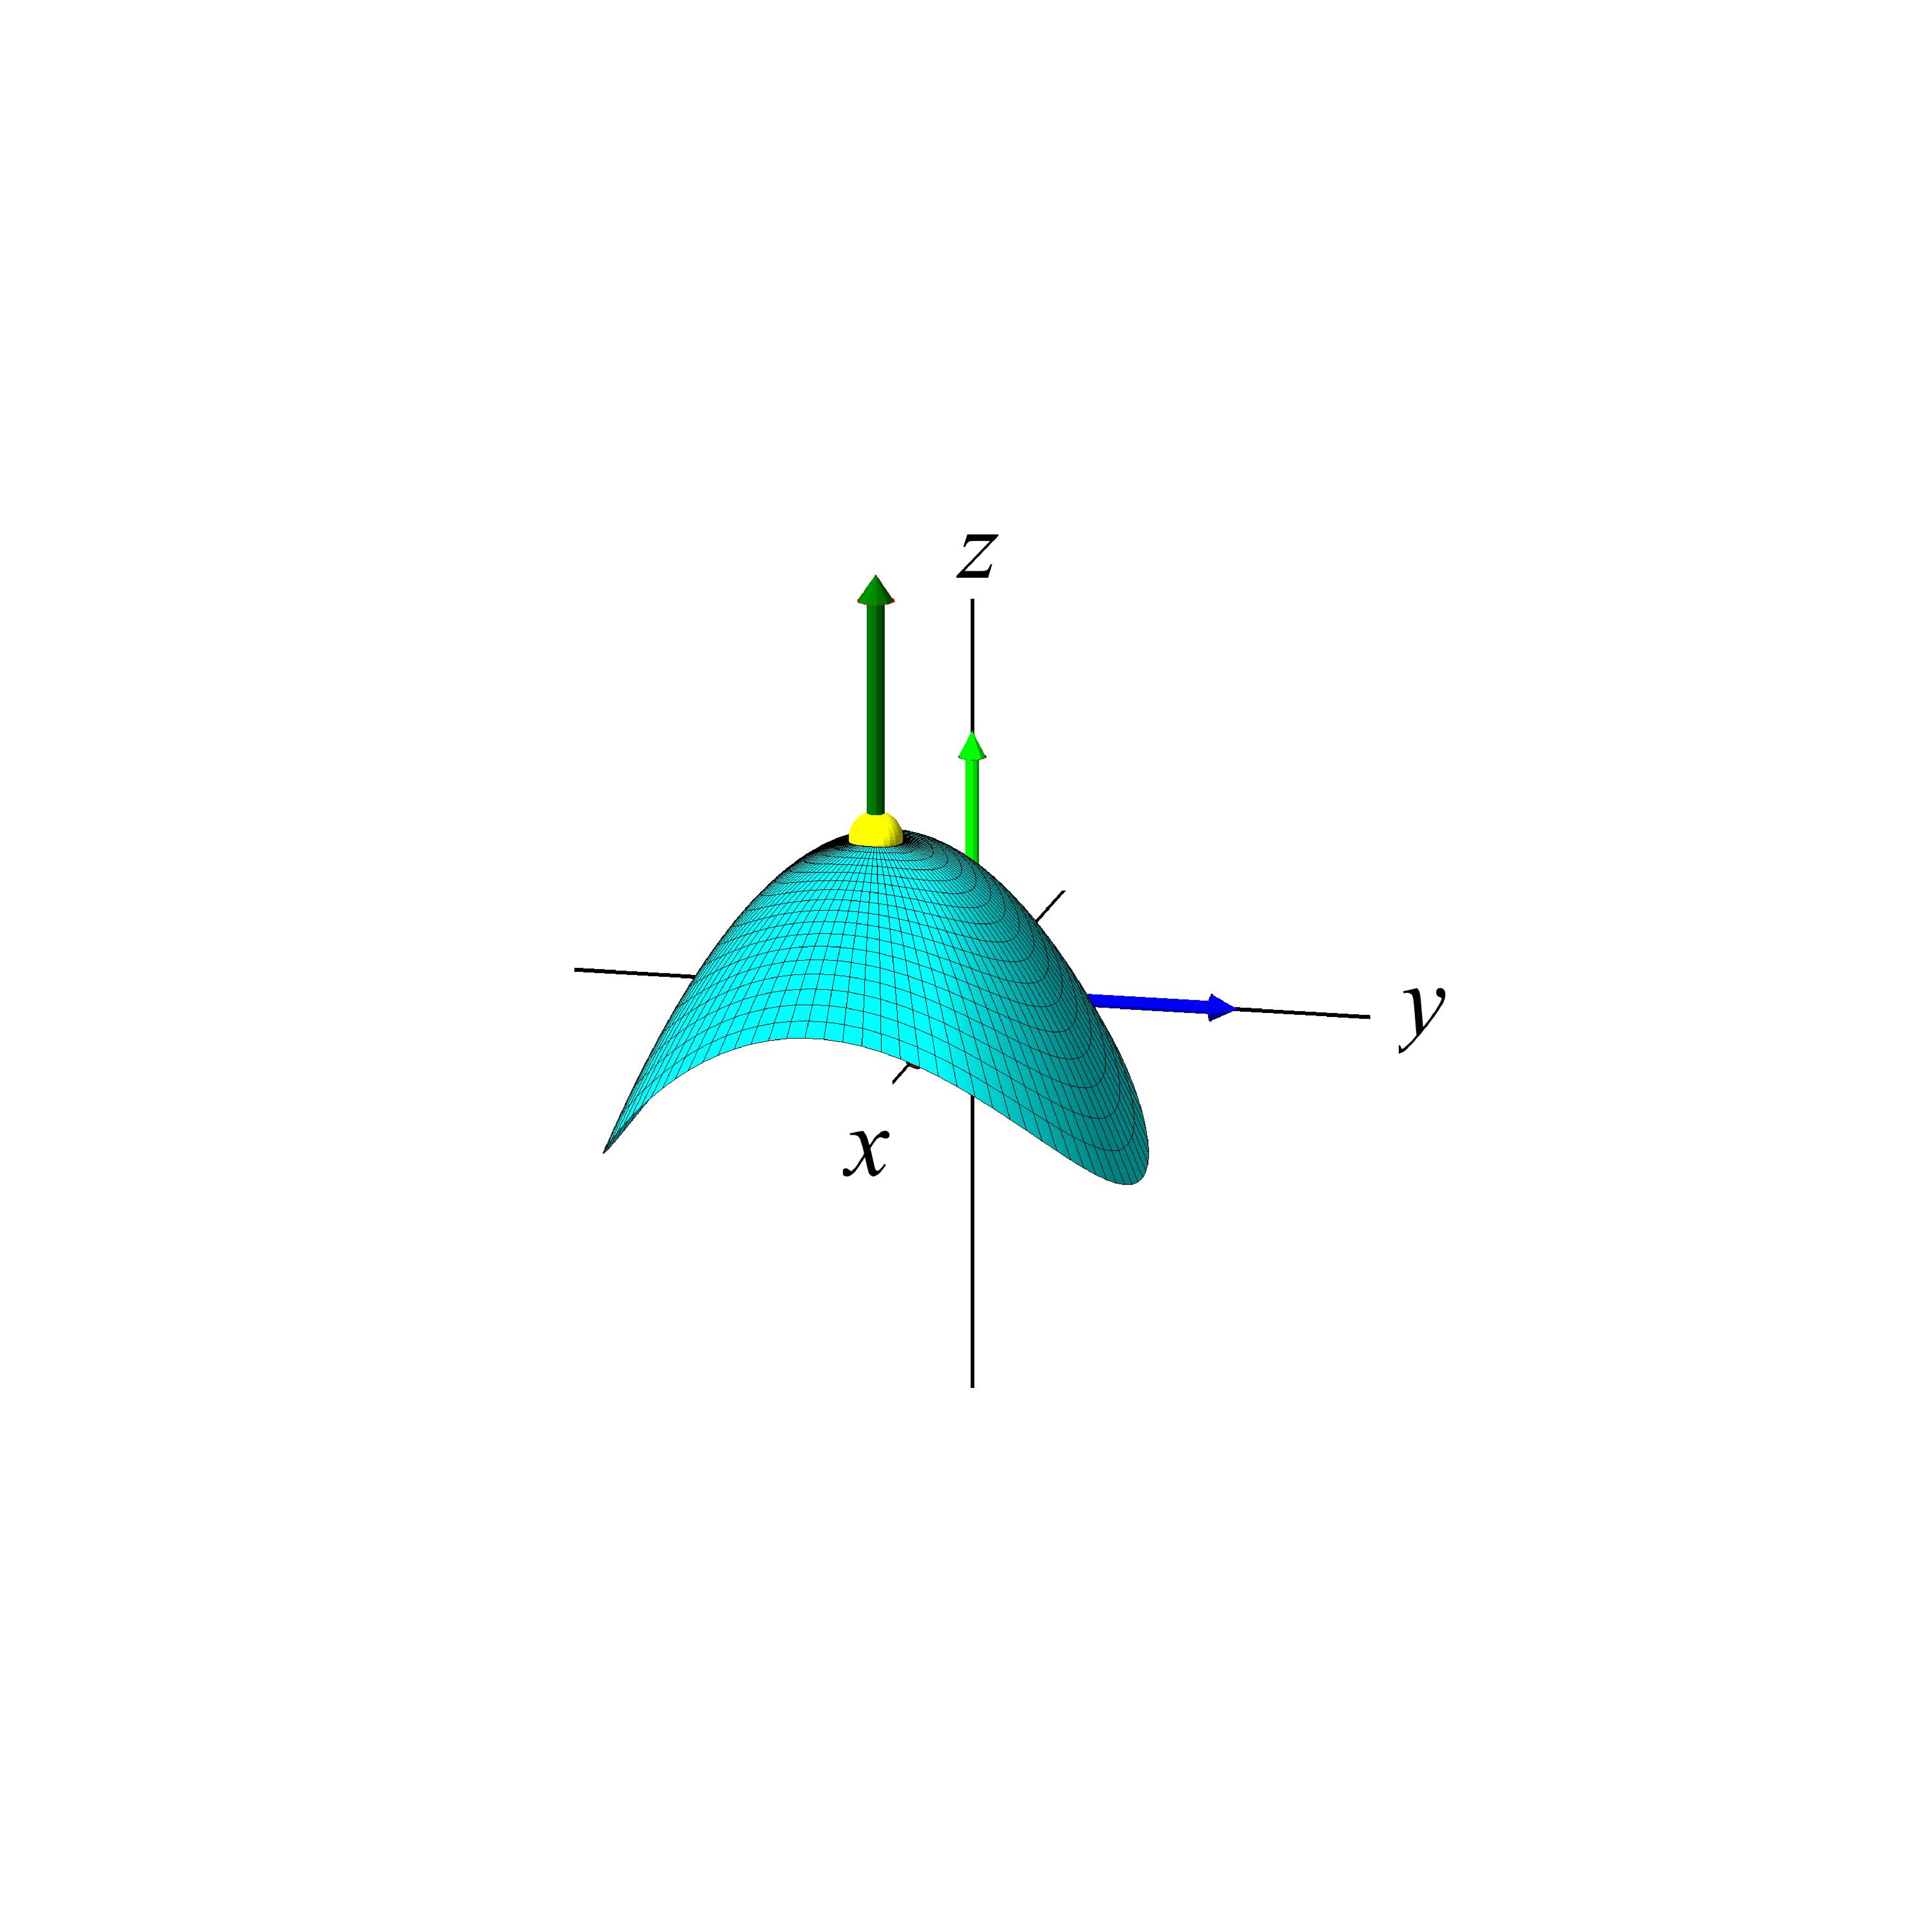
\includegraphics[height=55mm]{plotVar2App2.pdf}  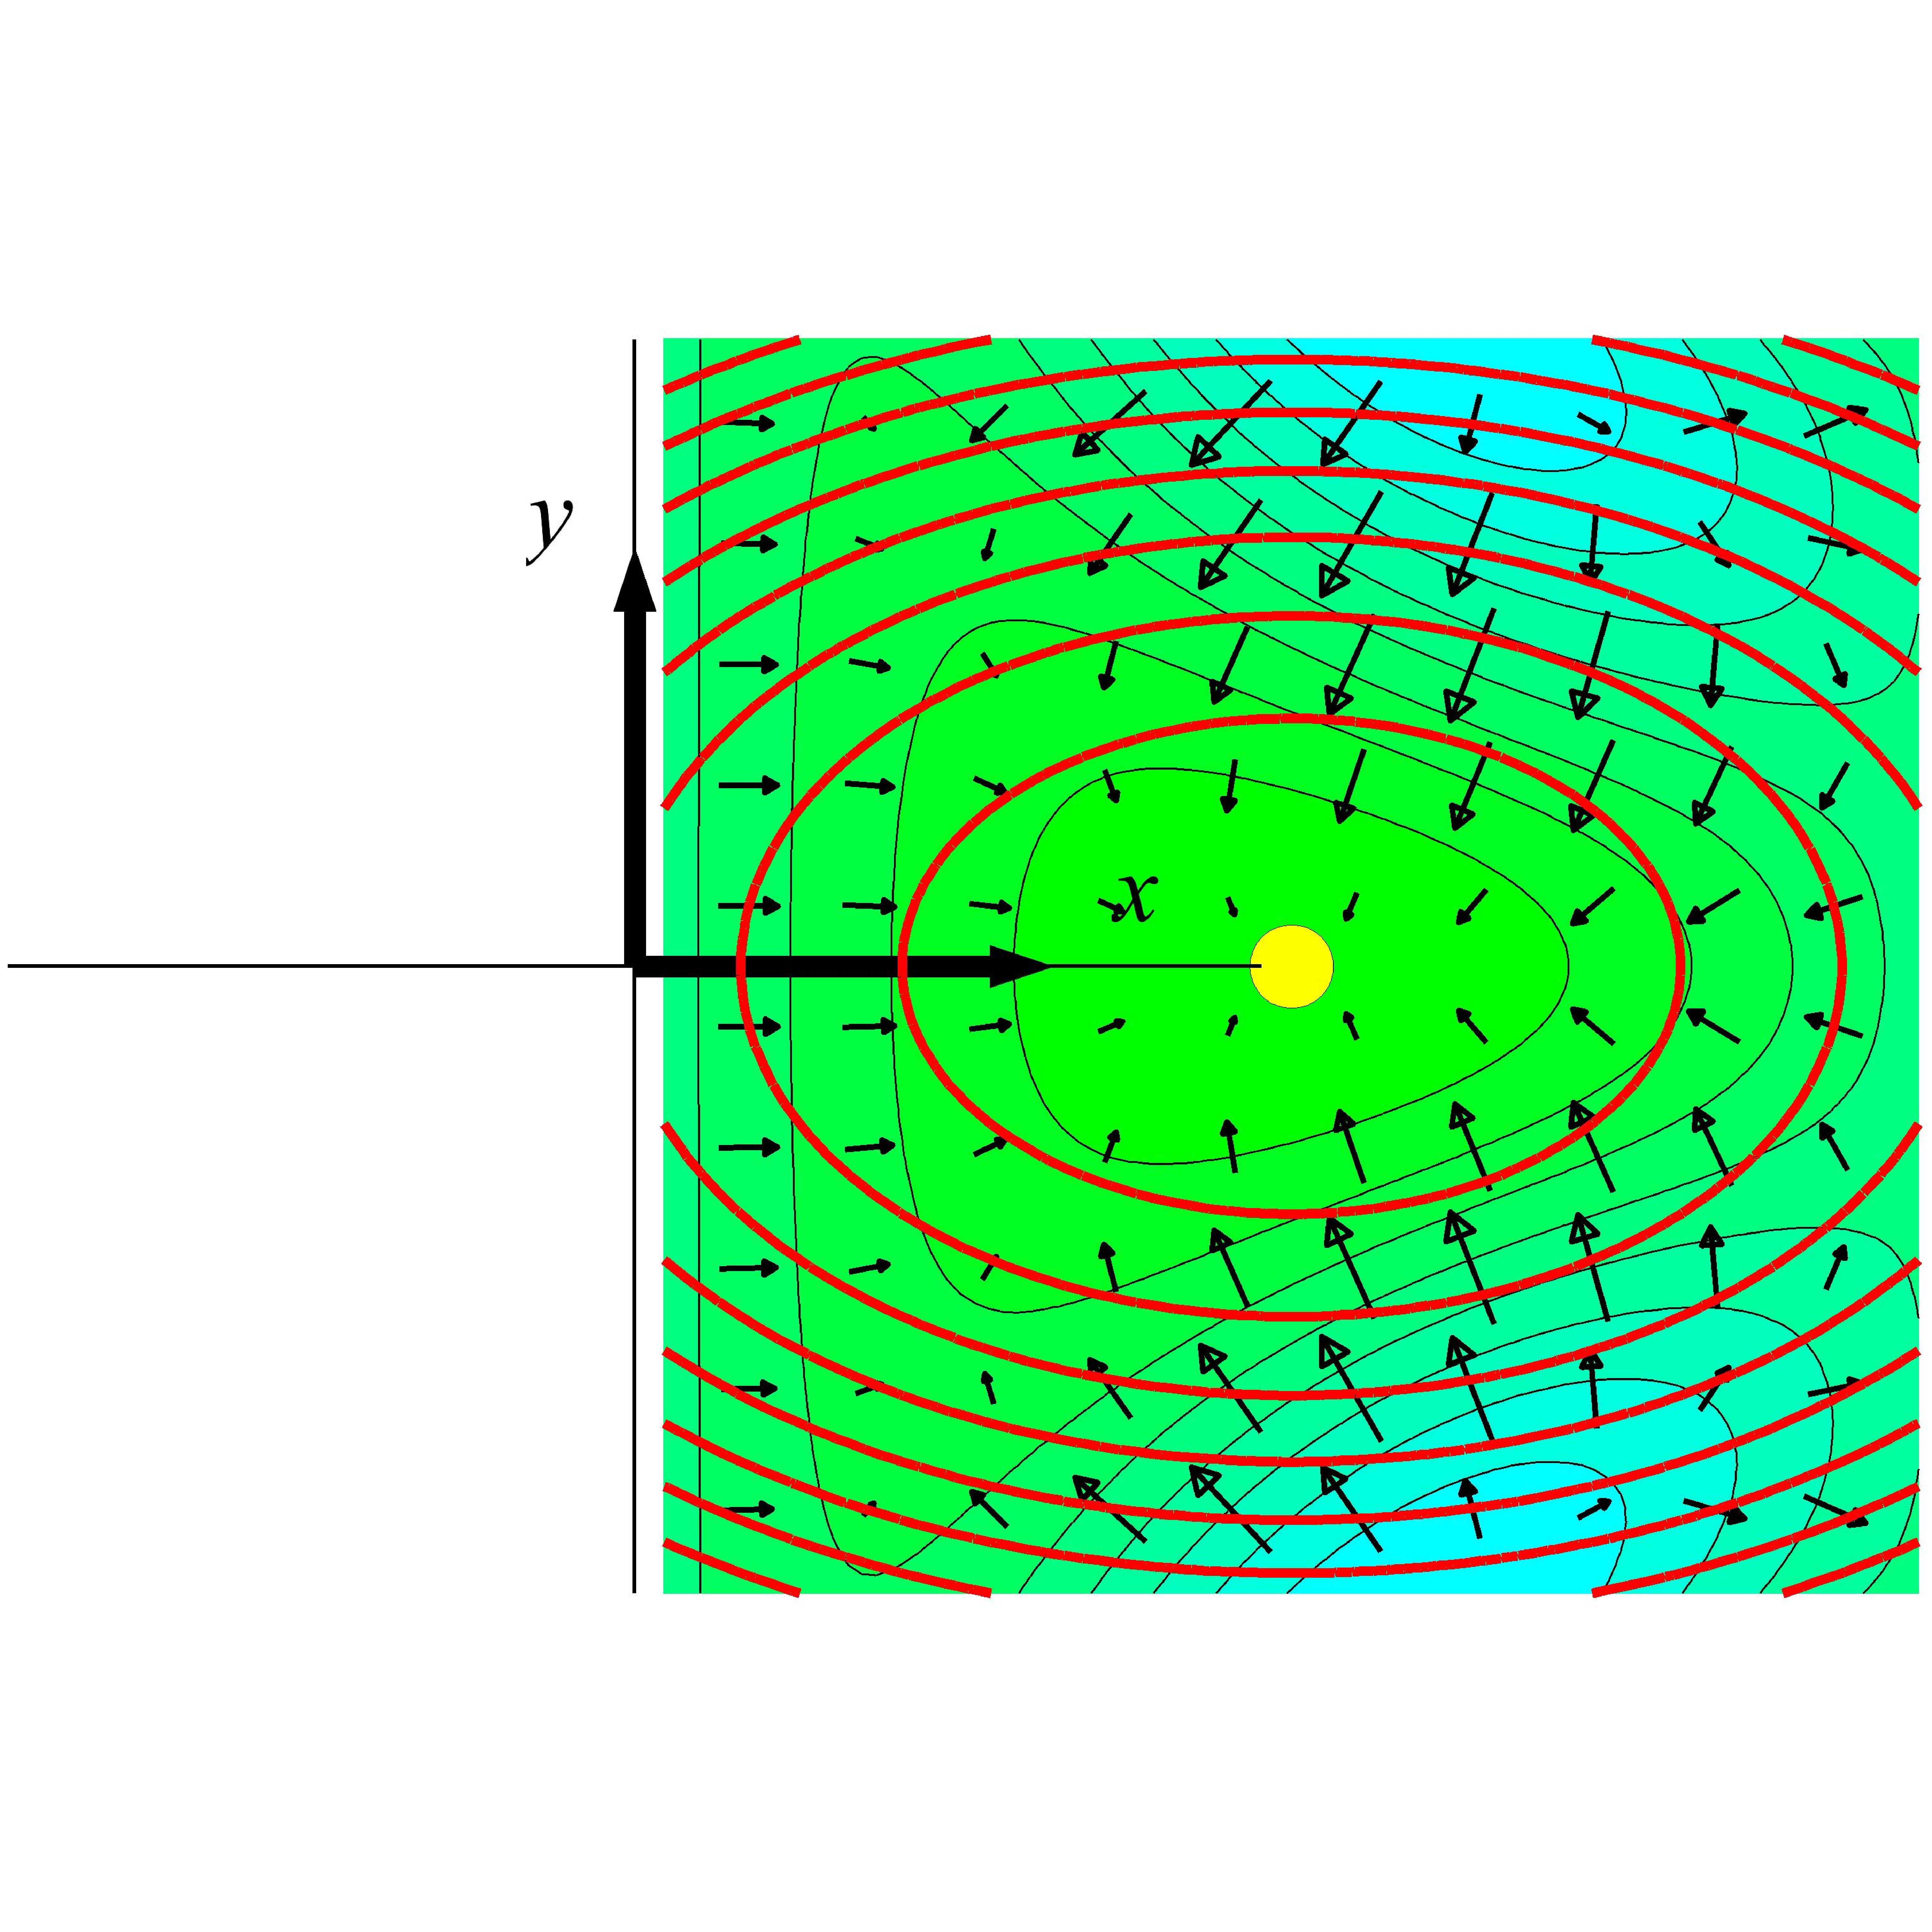
\includegraphics[height=55mm]{plotGrad2.pdf} }
\begin{center}
\caption{Til venstre: Grafen for funktionen $f(x,y) = \sin(x)\cdot\cos(x\cdot y)$.  I midten: Grafen for det approksimerende andengradspolynomium for $f(x,y)$ med udviklingspunkt i det stationære punkt $(\pi/2, 0)$. Til højre: Gradientvektorfeltet for funktionen $f(x,y)$, dens niveaukurver (sorte) samt niveaukurver for det approksimerende andengradspolynomium (røde).} \label{figStatInspec1}
\end{center}
\end{figure}



\begin{example}[Inspektion af stationært punkt] \label{exampStatInspec2}
Lad funktionen $f(x,y)$ være givet med følgende data i $\mathbb{R}^{2}$:
\begin{equation}
\begin{aligned}
f(x,y) &= 1+ x^{2} + (1-y)^{2} + x\cdot y \quad , \\
\bm{\nabla}f(x,y) &=  (2\cdot x + y, 2\cdot y -2 + x)  \quad .
\end{aligned}
\end{equation}
Så er $(x_{0}, y_{0}) = (-2/3 \, , \, 4/3) $ et stationært punkt for $f(x,y)$ og i det punkt har vi som i alle andre punkter
\begin{equation}
\bm{H}f(x_{0},y_{0}) = \left[
                                                                           \begin{array}{cc}
                                                                             2 & 1 \\
                                                                             1 & 2\\
                                                                           \end{array}
                                                                         \right]
\end{equation}
I det stationære punkt har Hesse-matricen således egenværdierne $3$ og $1$. Vi konkluderer, at det stationære punkt er et egentligt lokalt minimumpunkt for $f(x,y)$ i overensstemmelse med inspektion af figur \ref{figStatInspec2} og i overensstemmelse med hjælpesætning\ref{lemmaEkstrema2Var}.

Det approksimerende andengradspolynomium for $f(x,y)$ med udviklingspunkt i det stationære punkt $(x_{0}, y_{0})= (\pi/2, 0)$ er funktionen selv:
\begin{equation}
P_{2, (-2/3 \, , \, 4/3)}(x,y) =   f(x,y)      \quad.
\end{equation}
\end{example}

\begin{figure}[ht]
\centerline{ 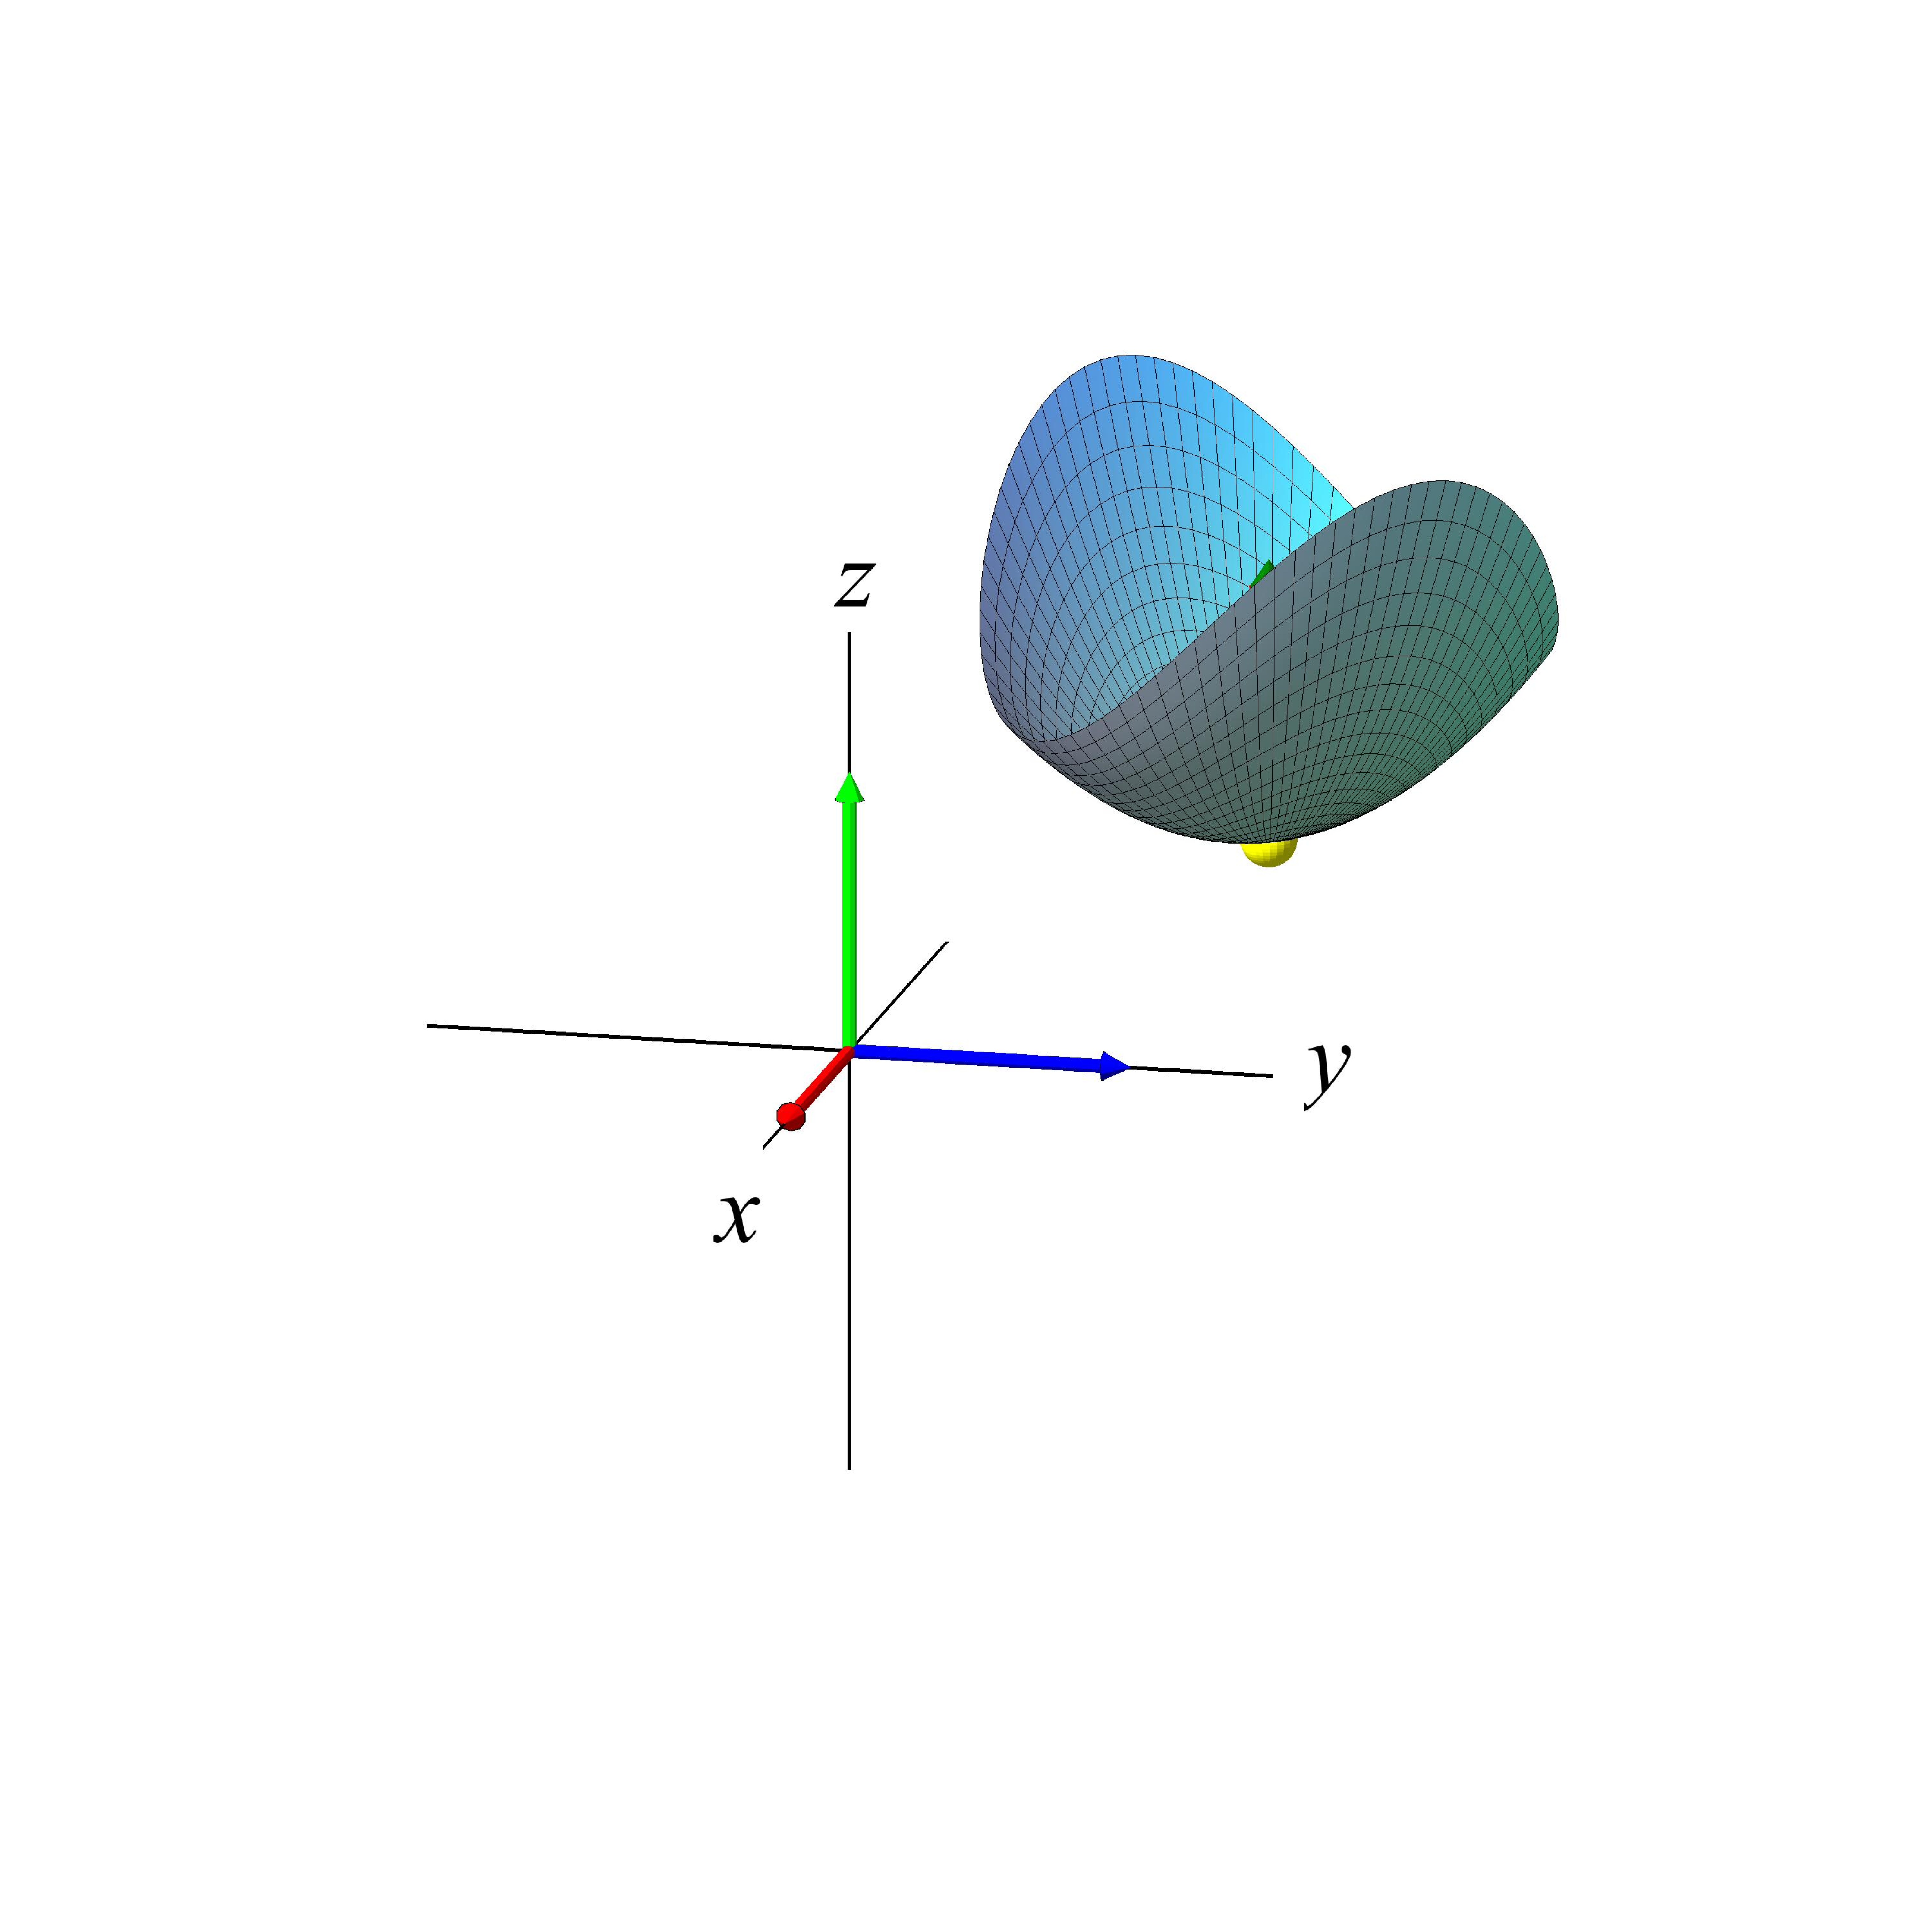
\includegraphics[height=75mm]{plotVar2Fig4.pdf} 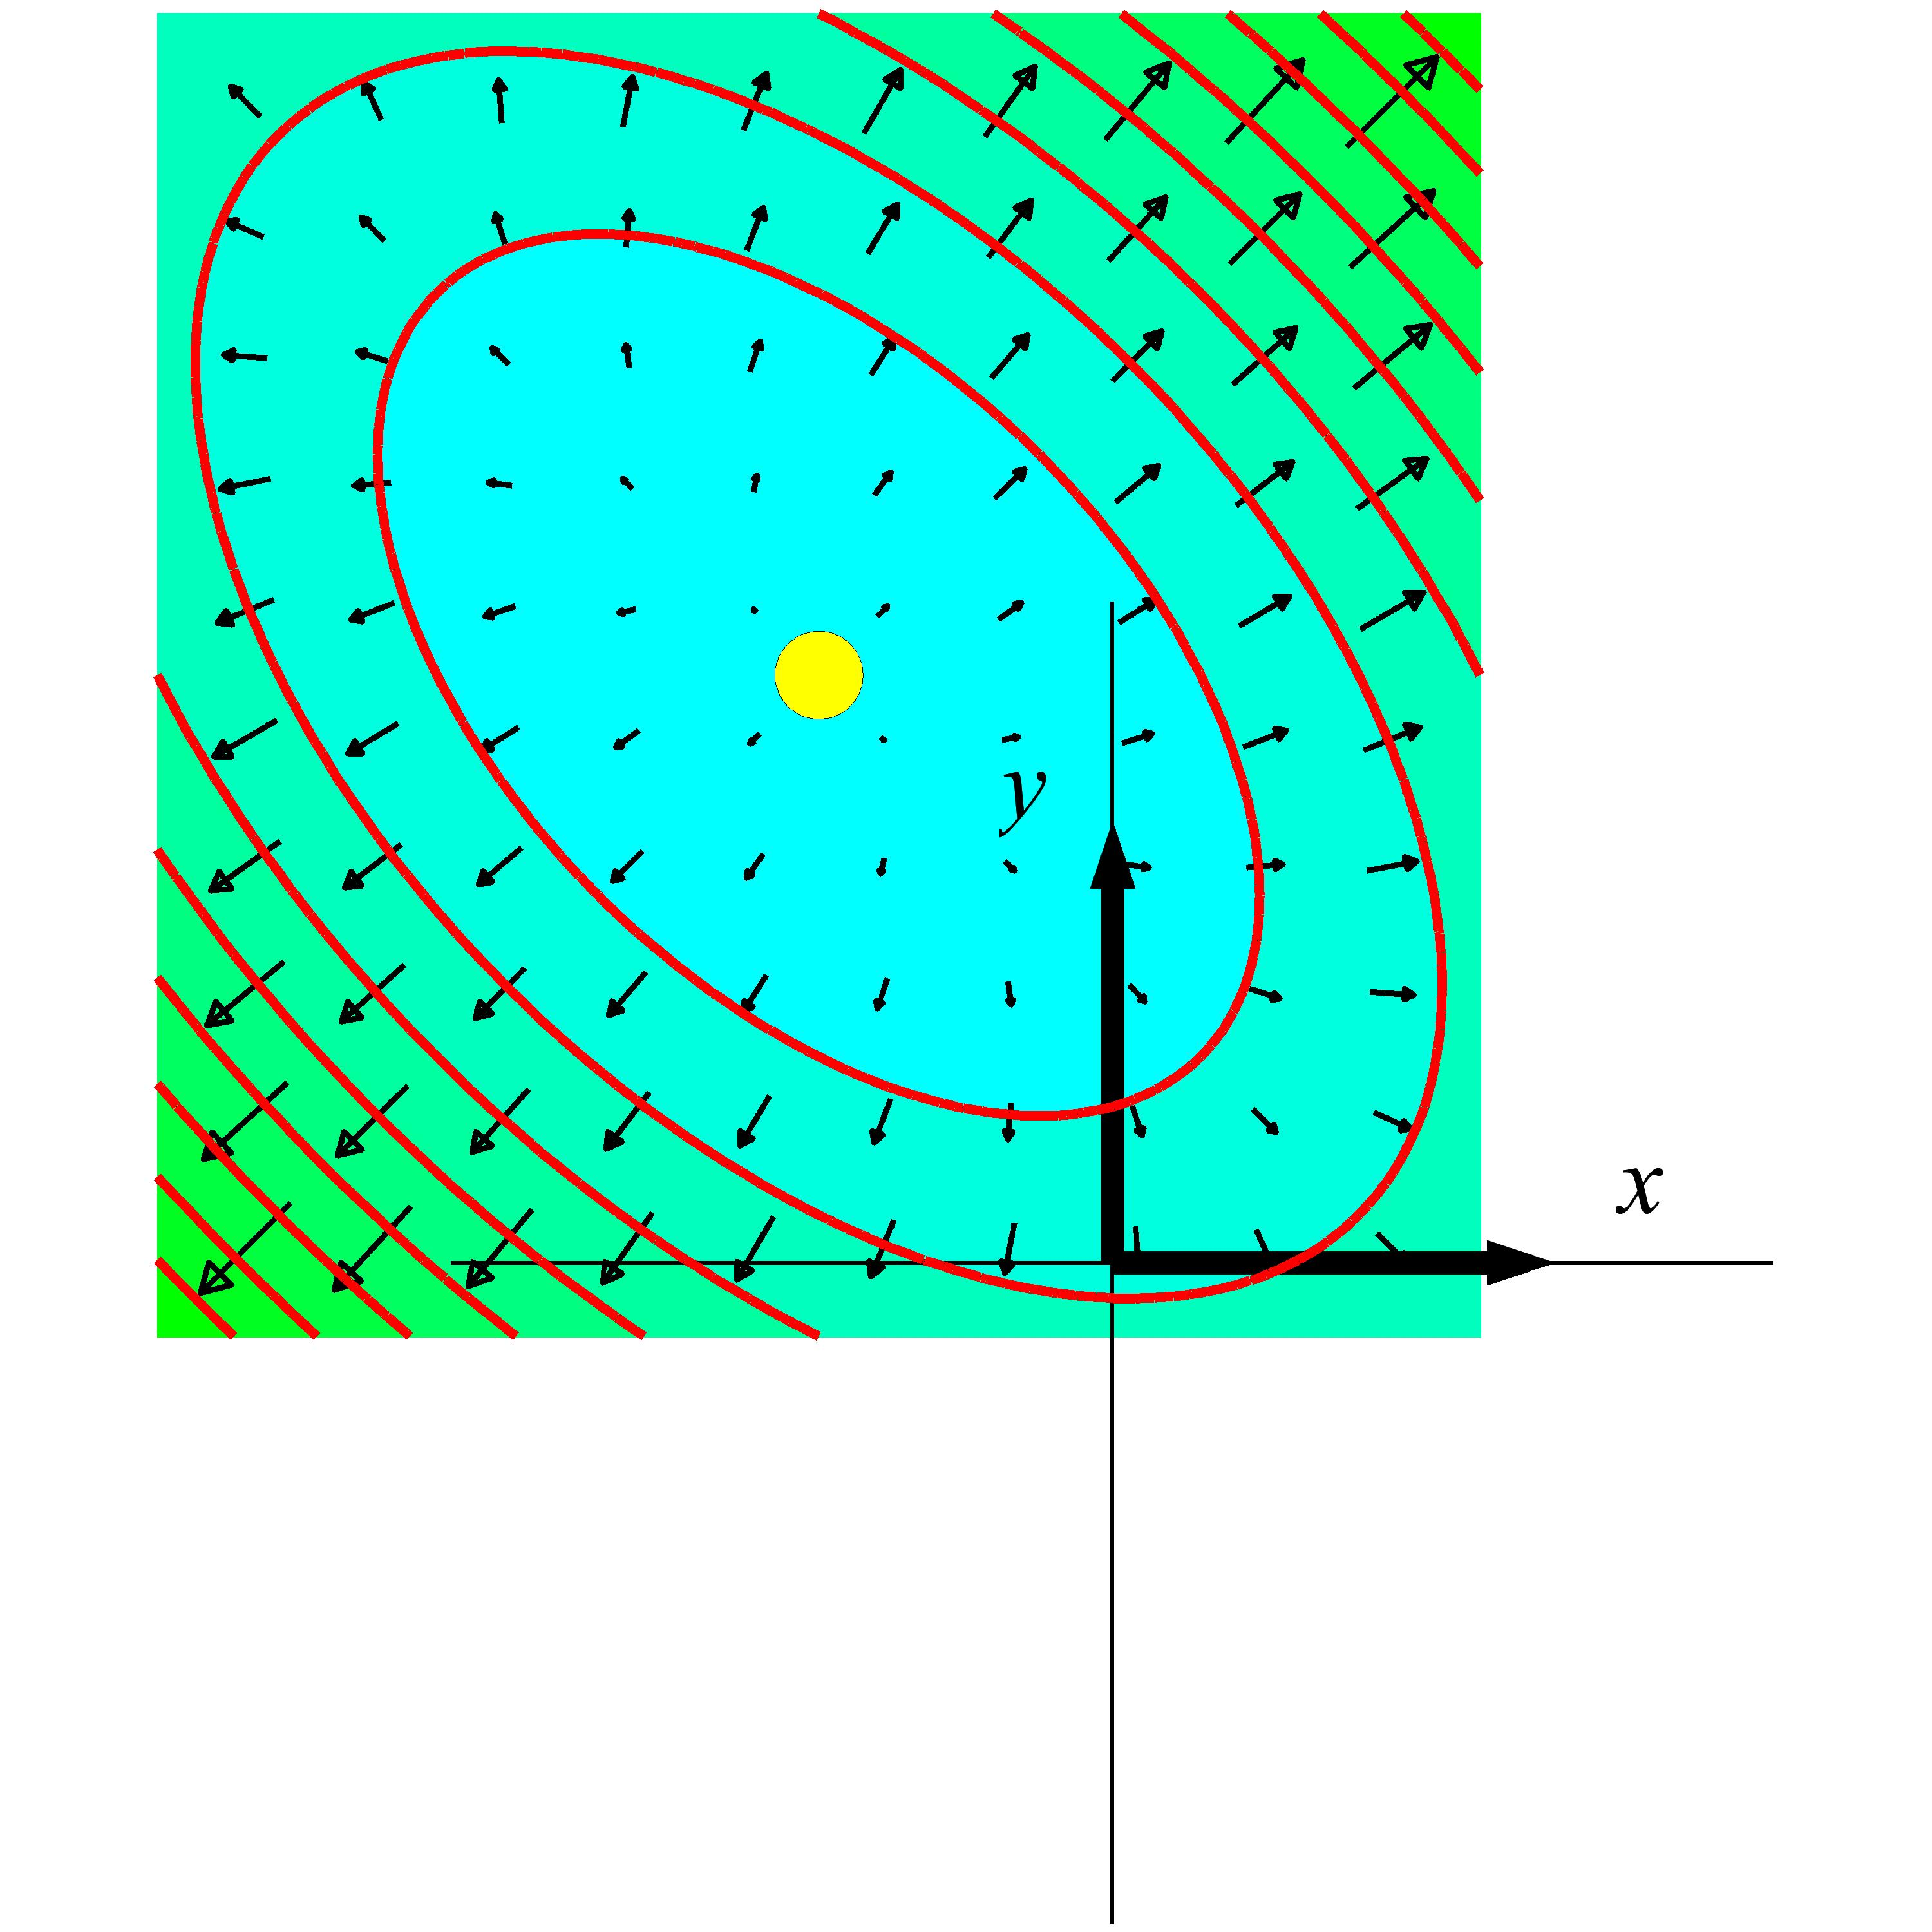
\includegraphics[height=55mm]{plotGrad4.pdf} }
\begin{center}
\caption{Til venstre: Grafen for funktionen $f(x,y) = 1+ x^{2} + (1-y)^{2} + x\cdot y $.  Til højre: Gradientvektorfeltet for funktionen $f(x,y)$, og dens niveaukurver (røde) omkring det stationære punkt $(x_{0}, y_{0}) = (-2/3 \, , \, 4/3)$. Bemærk, at funktionen er sit eget approksimerende andengradspolynomium med udviklingspunkt i det stationære punkt.} \label{figStatInspec2}
\end{center}
\end{figure}

%%%%%%%%%%%%%%%%%%%%%%%%%%%%%%%%%%%%%%%%%%%%%%%%%%%
%%%%%%%%%%%%%%%%%%%%%%%%%%%%%%%%%%%%%%%%%%%%%%%%%%%
%%%%%%%%%%%%%%%%%%%%%%%%%%%%%%%%%%%%%%%%%%%%%%%%%%%




\begin{example}[Inspektion af stationært punkt] \label{exampStatInspec3}
Lad funktionen $f(x,y)$ være givet med følgende data i $\mathbb{R}^{2}$:
\begin{equation}
\begin{aligned}
f(x,y) &= \frac{1}{2}\cdot \sin(\pi\cdot x^{2} + \pi \cdot y^{2}) \quad , \\
\bm{\nabla}f(x,y) &=  (\pi \cdot x\cdot \cos(\pi\cdot x^{2} + \pi \cdot y^{2}), \pi \cdot y\cdot \cos(\pi\cdot x^{2} + \pi \cdot y^{2}) ) \quad .
\end{aligned}
\end{equation}
Så er $(x_{0}, y_{0}) = (0, 1/\sqrt{2}) $ et (blandt rigtig mange) stationært punkt for $f(x,y)$ og i det punkt har vi
\begin{equation}
\bm{H}f(x_{0},y_{0}) = \left[
                                                                           \begin{array}{cc}
                                                                             0 & 0 \\
                                                                             0 & -\pi^{2}\\
                                                                           \end{array}
                                                                         \right]
\end{equation}
I det stationære punkt har Hesse-matricen således egenværdierne $0$ og $-\pi^{2}$. Hjælpesætning \ref{lemmaEkstrema2Var} kan derfor ikke afgøre, om vi har lokalt maksimum eller minimum i punktet. Men da $f(0, 1/\sqrt{2}) = 1/2$, som er den maksimale værdi $f(x,y)$ kan antage, så er $(0, 1/\sqrt{2})$ et lokalt masimumpunkt for $f(x,y)$ men det er ikke et egentligt lokalt maksimumpunkt fordi alle punkter på hele cirklen $x^{2} + y^{2} = 1/2$ er også lokale maksimumpunkter for $f(x,y)$. Se også figur \ref{figStatInspec3}.


\end{example}

\begin{figure}[ht]
\centerline{ 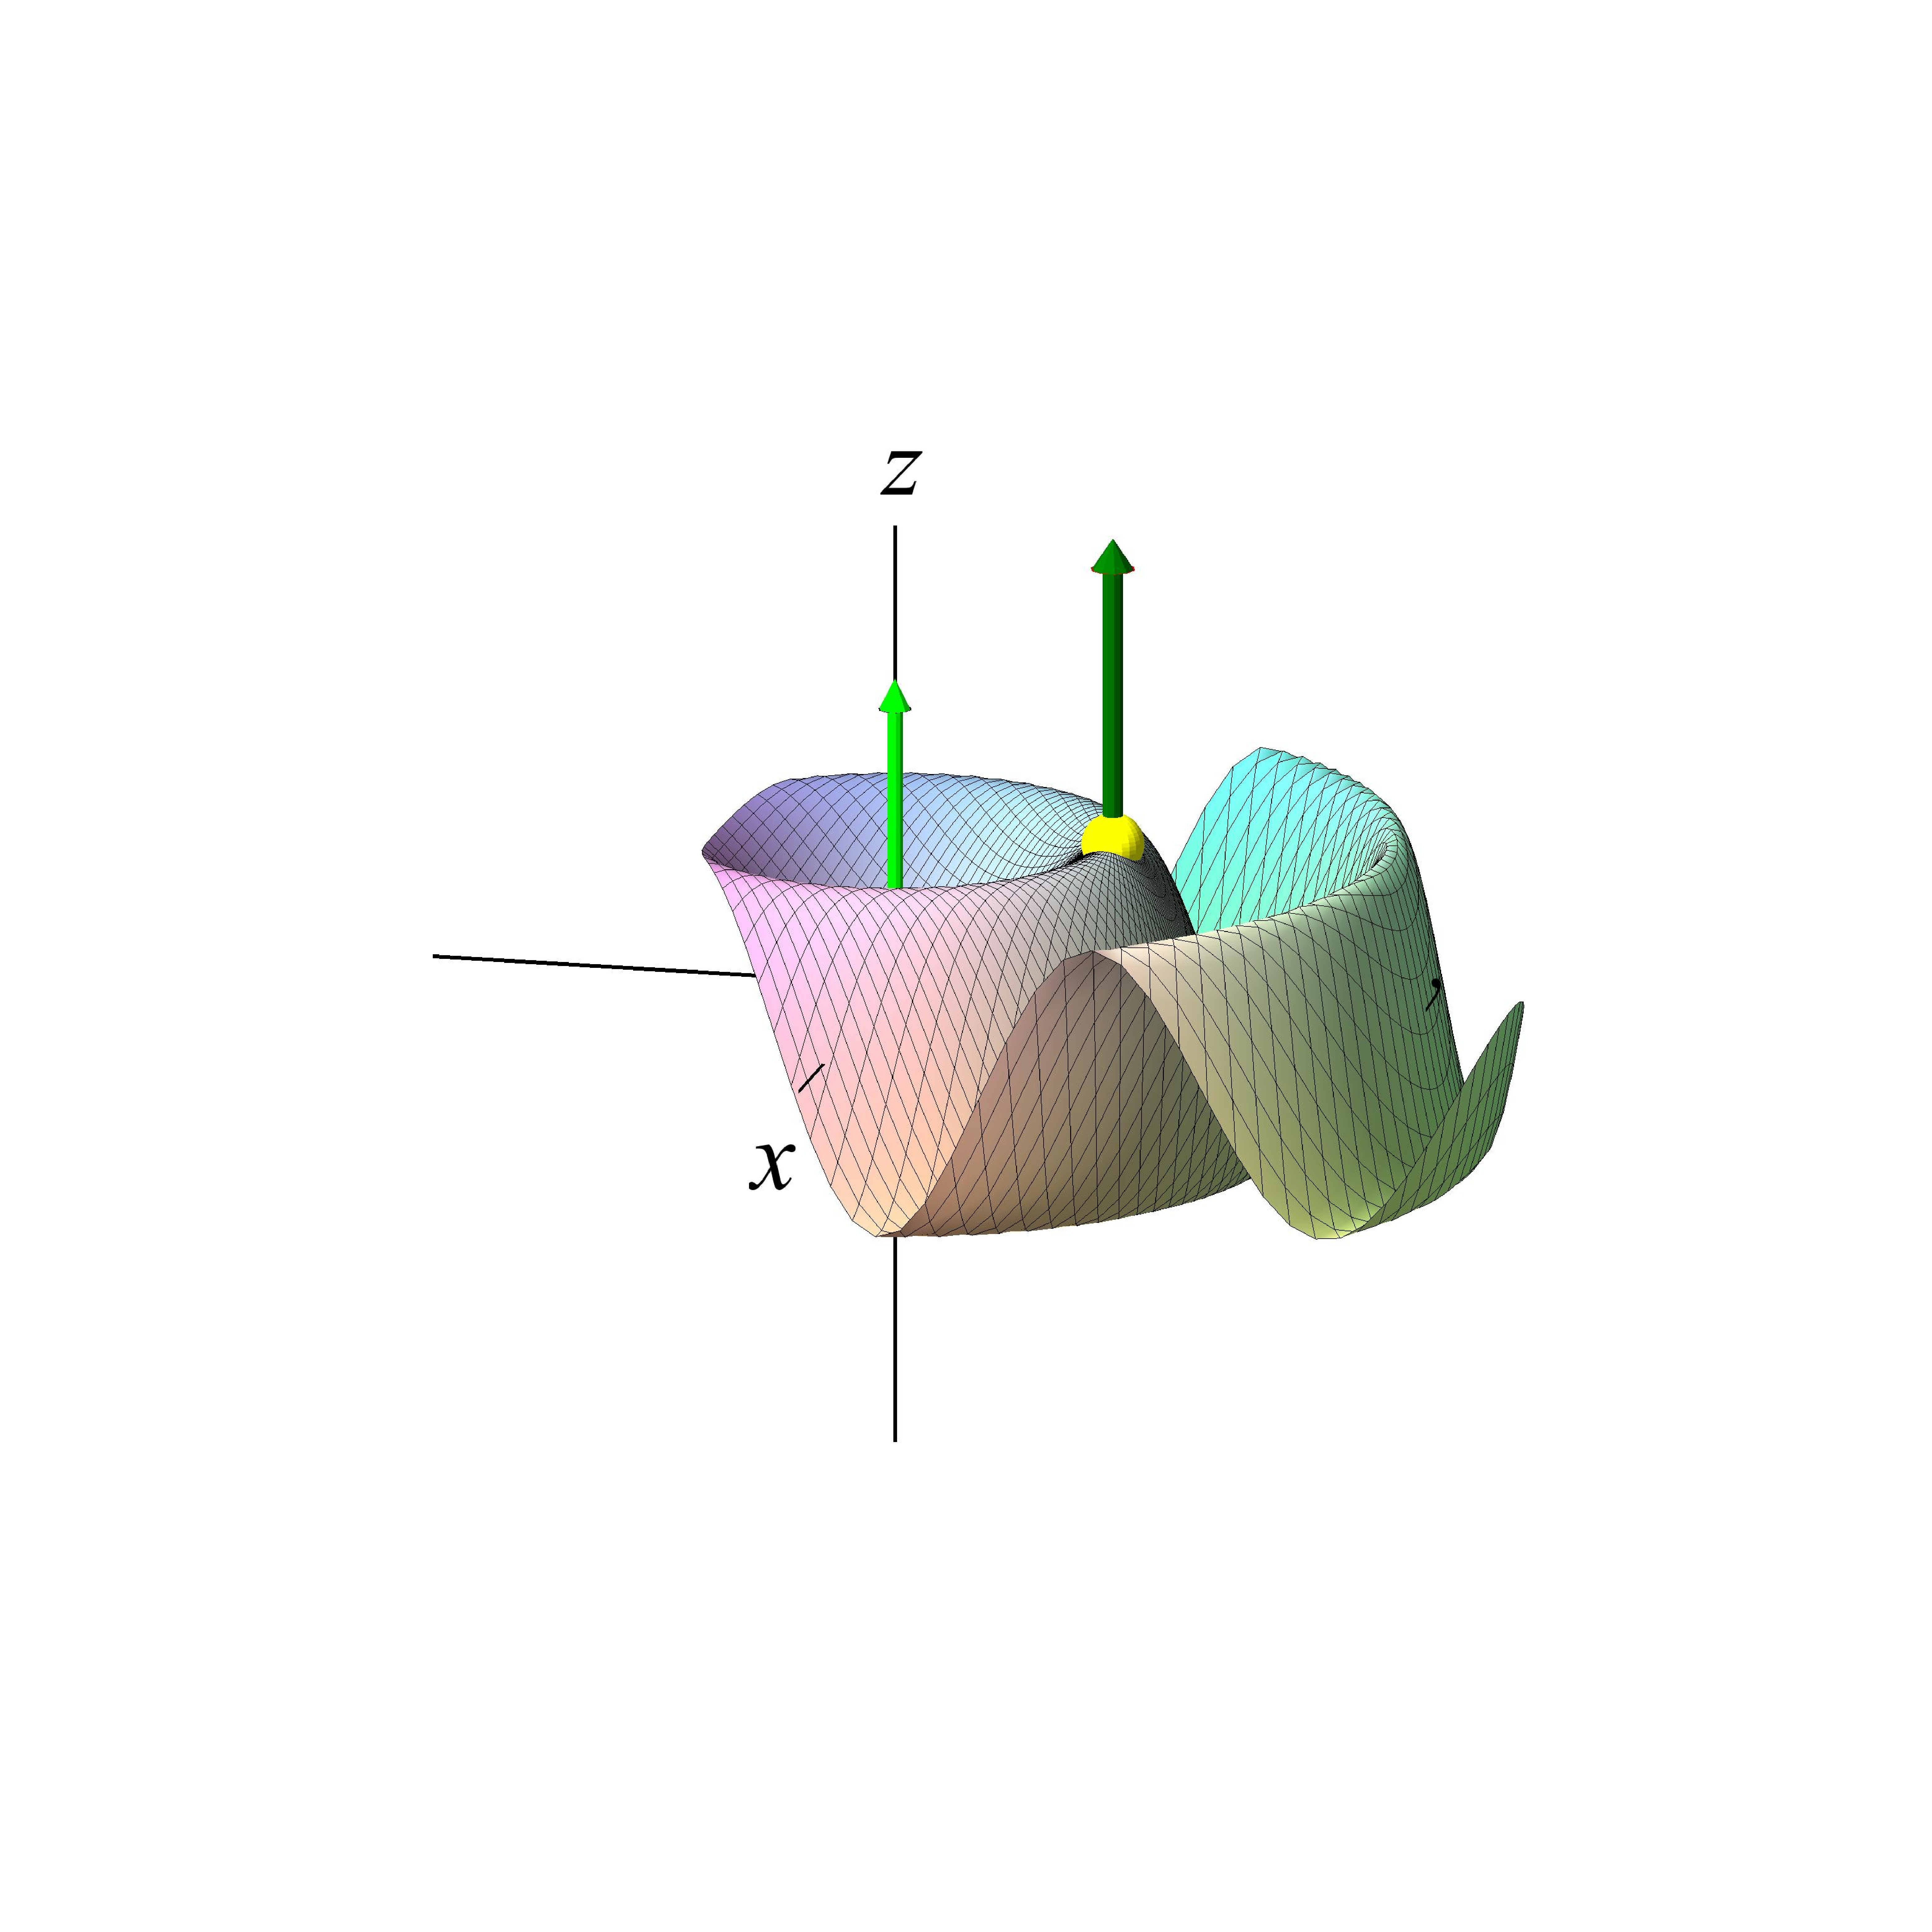
\includegraphics[height=55mm]{plotVar2Fig7.pdf}  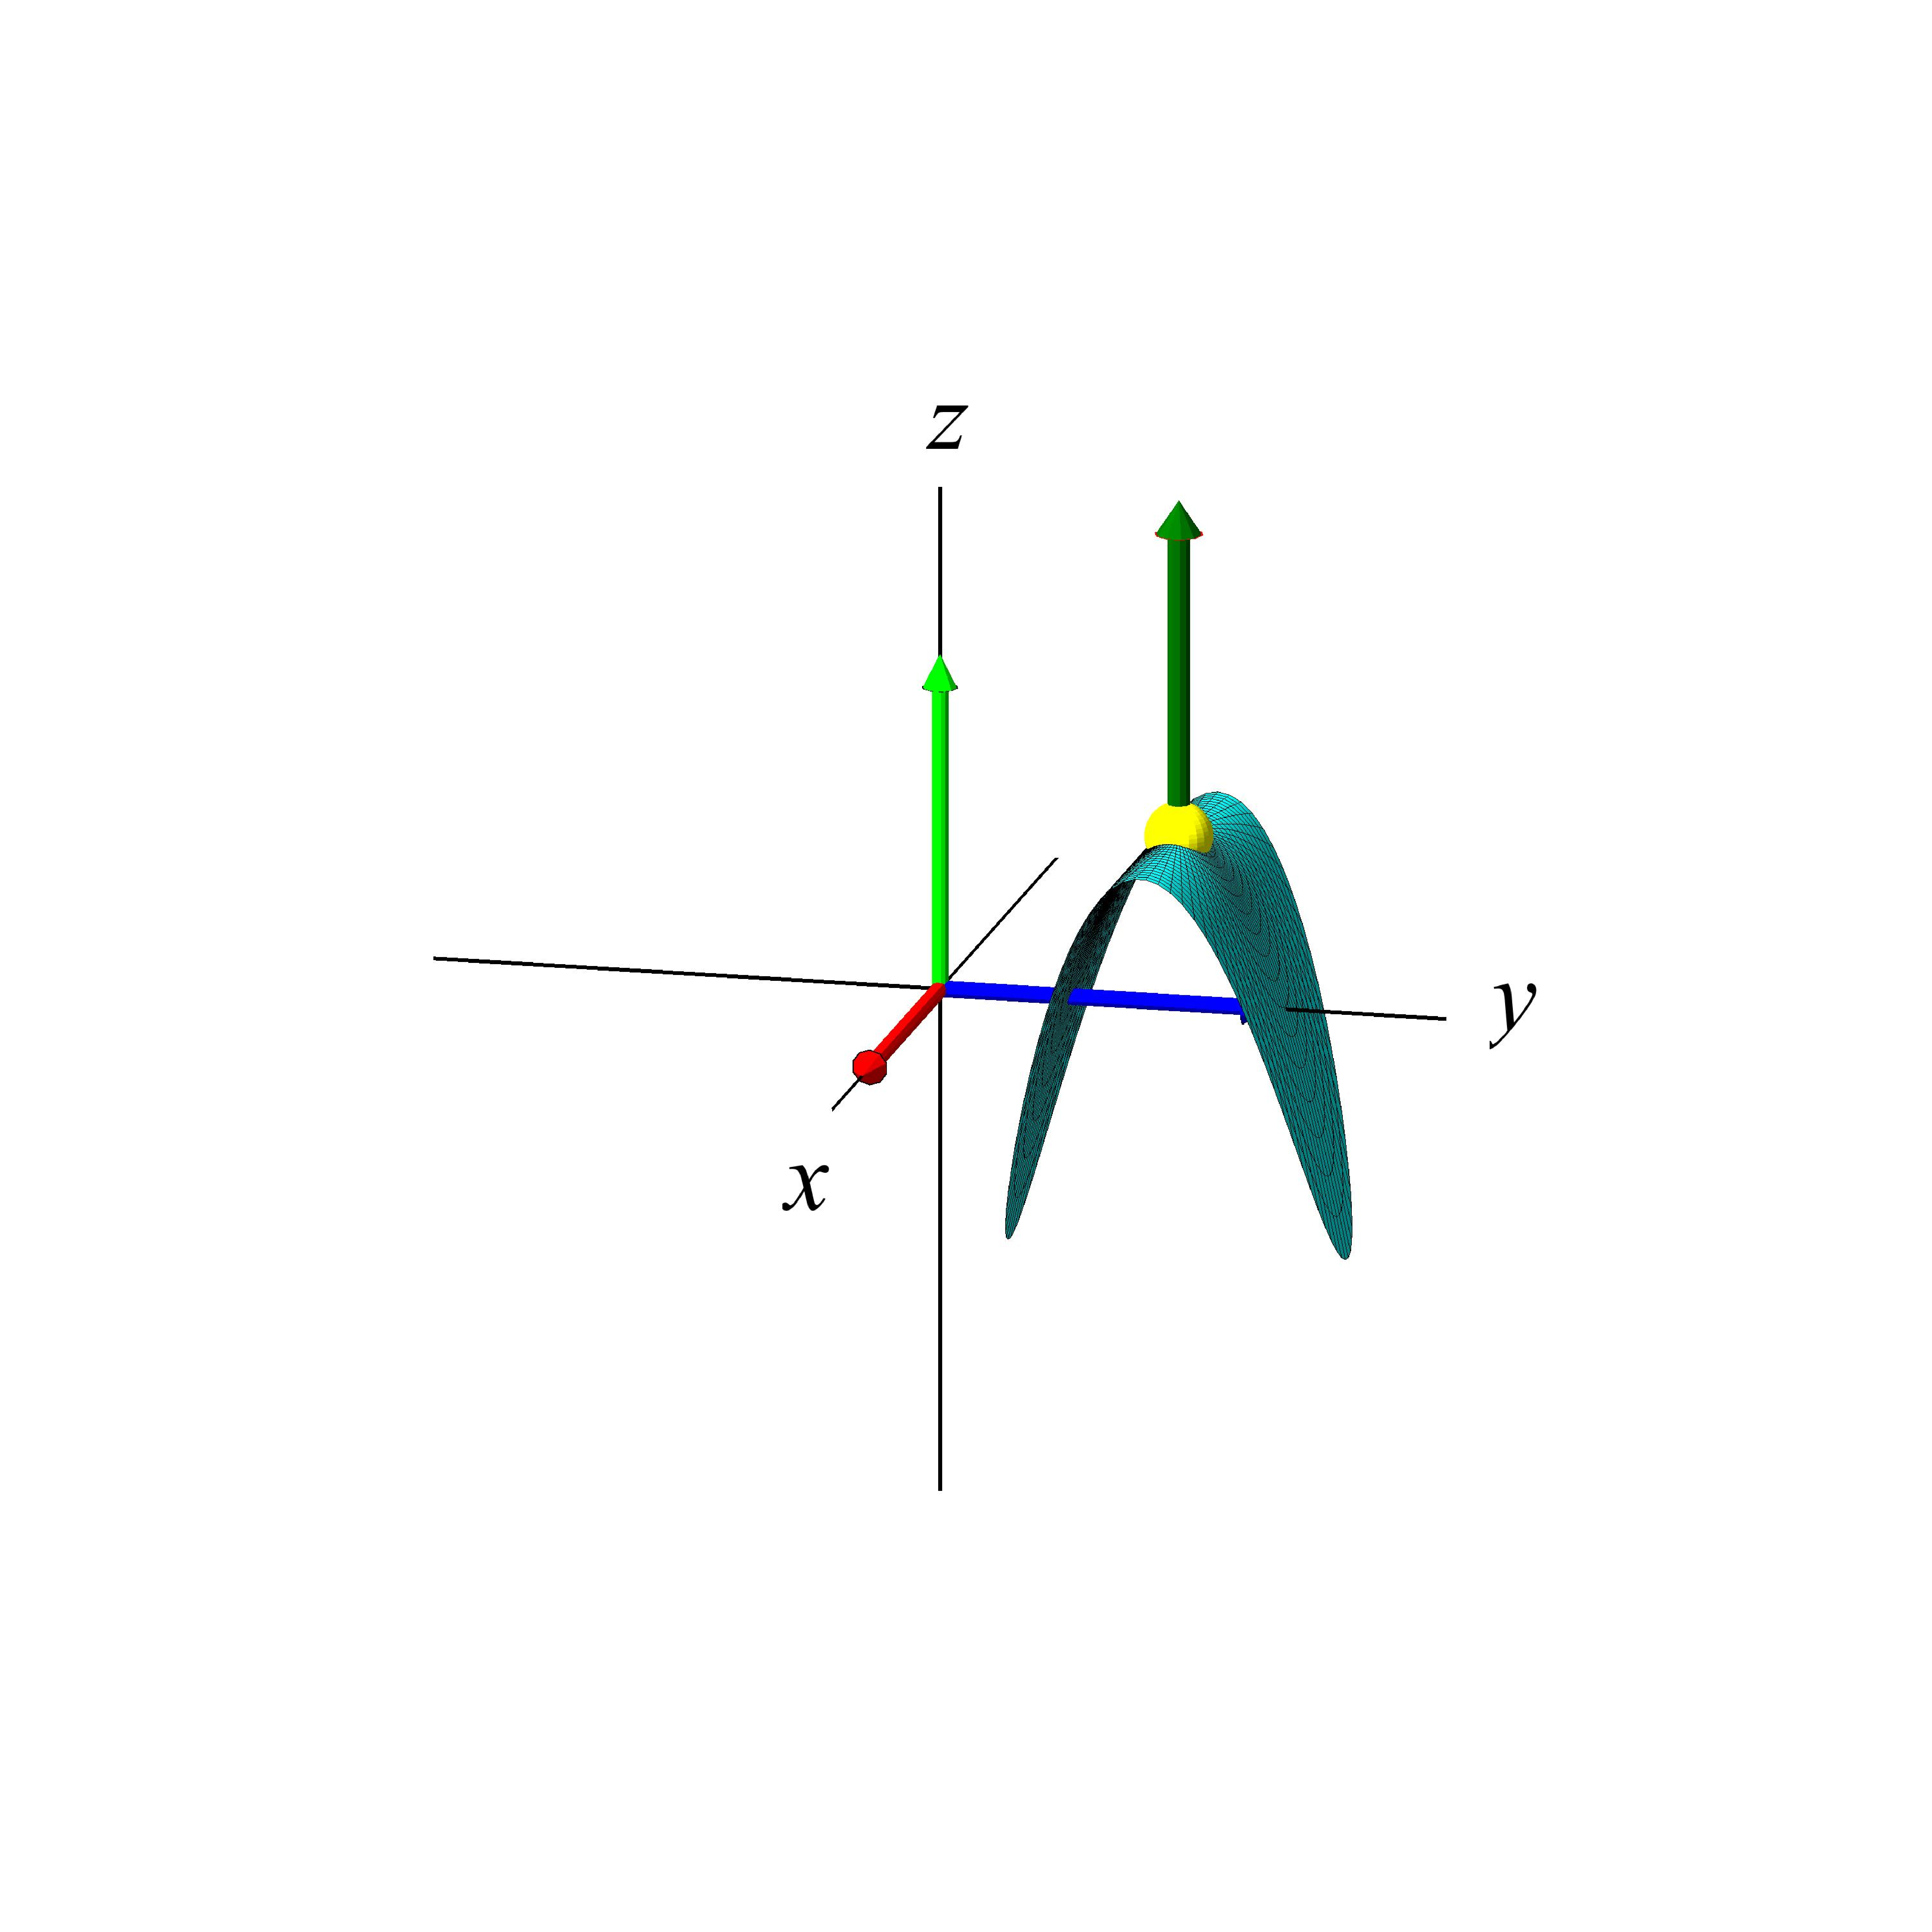
\includegraphics[height=55mm]{plotVar2App7.pdf}  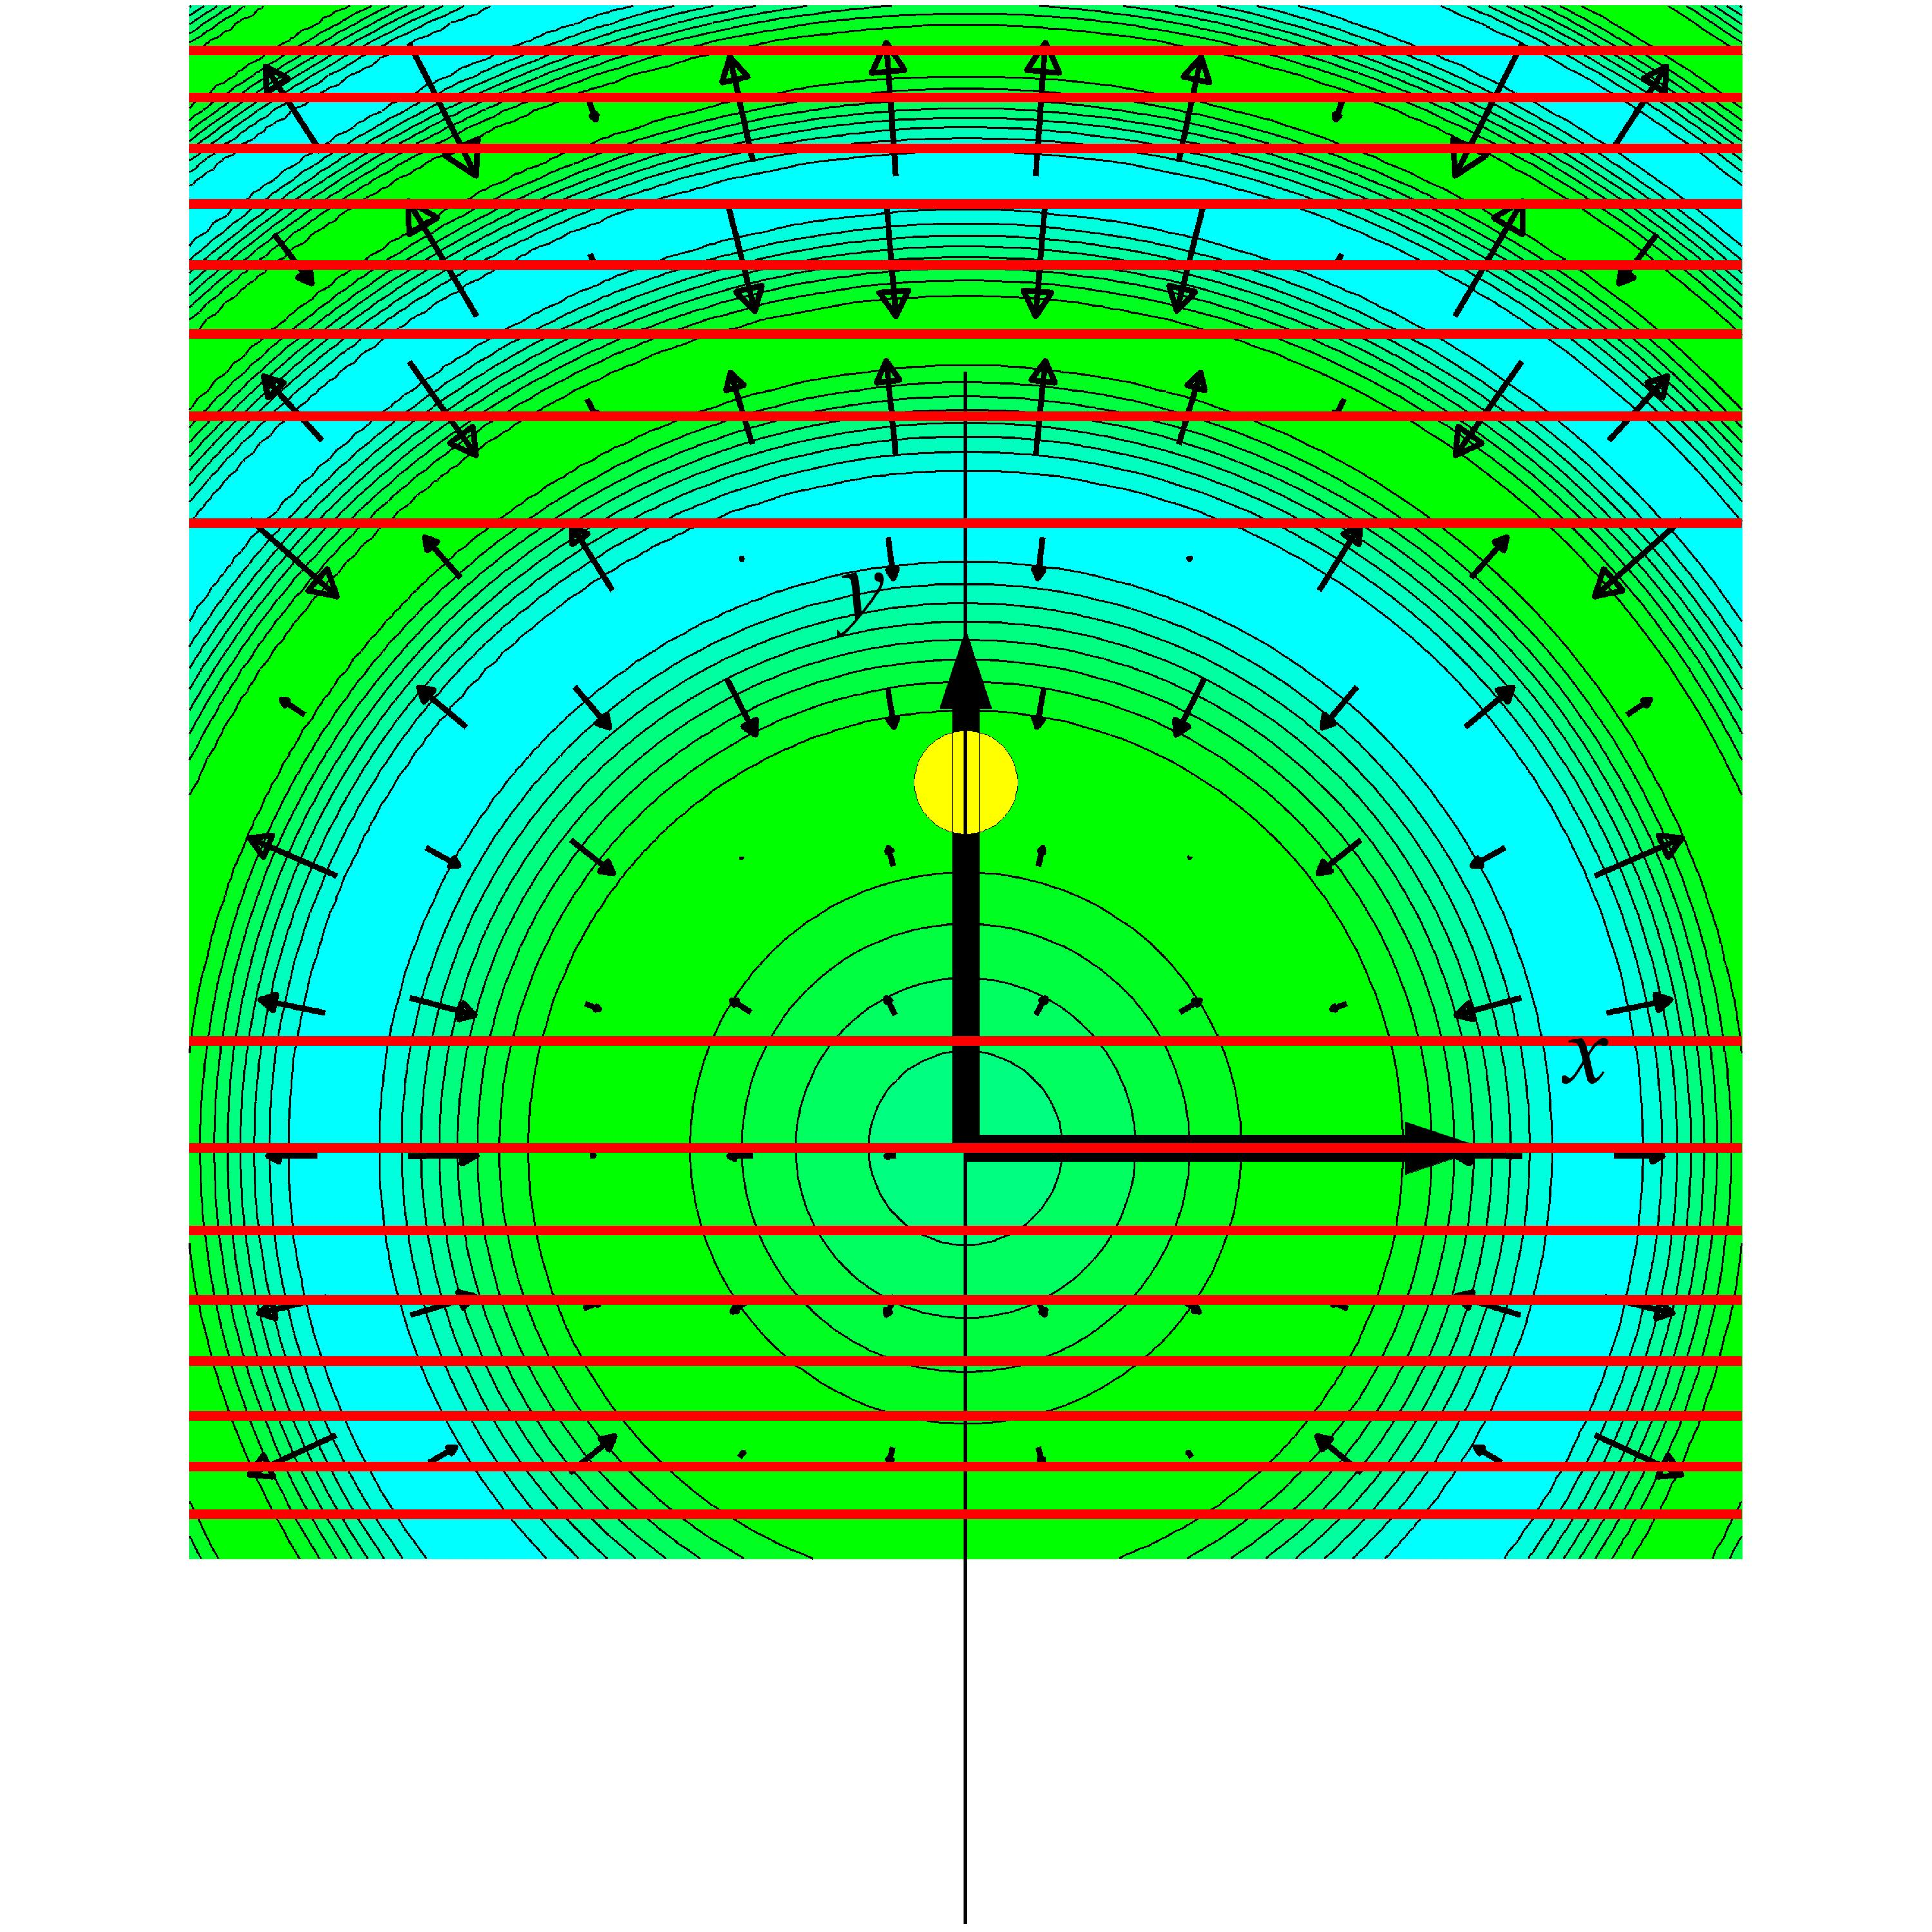
\includegraphics[height=55mm]{plotGrad7.pdf}}
\begin{center}
\caption{Til venstre: Grafen for funktionen $f(x,y) = \frac{1}{2}\cdot \sin(\pi\cdot x^{2} + \pi \cdot y^{2}) $. I midten: Det approksimerende andengradspolynomium for funktionen med udviklingspunkt $(0, 1/\sqrt{2})$. Til højre: Gradientvektorfeltet for funktionen $f(x,y)$, og dens niveaukurver (sorte) samt niveaukurver for det approksimerende andengradspolynomium (røde) omkring det stationære punkt $(x_{0}, y_{0}) = (0, 1/\sqrt{2})$.} \label{figStatInspec3}
\end{center}
\end{figure}




\begin{example}[Inspektion af stationært punkt] \label{exampStatInspec4}
Vi ser på en  funktion $f(x,y)$ som er defineret ved
\begin{equation}
f(x,y) =  \frac{1}{5}\cdot \left( 1 - (1-y)^{2} -x^{2}\right) \cdot \left( 4 - (2-y)^{2} - x^{2} \right) \quad .
\end{equation}
Så er $(x_{0}, y_{0}) = (0, 0) $ et stationært punkt for $f(x,y)$ og i det punkt har vi
\begin{equation}
\bm{H}f(0,0) = \left[
                                                                           \begin{array}{cc}
                                                                             0 & 0 \\
                                                                             0 & 16/5\\
                                                                           \end{array}
                                                                         \right]
\end{equation}
I det stationære punkt har Hesse-matricen således egenværdierne $0$ og $16/5$. Hjælpesætning \ref{lemmaEkstrema2Var} kan derfor ikke afgøre, om vi har lokalt maksimum eller minimum i punktet.  Det er dog forholdsvis let at se, at der vilkårligt tæt på $(0,0)$ findes punkter $(x,y)$ hvor funktionsværdierne $f(x,y)$ er negative og at der også vilkårligt tæt på $(0,0)$ findes punkter $(x,y)$ hvor funktionsværdierne $f(x,y)$ er positive. Se figur \ref{figStatInspec4}. Det stationære punkt $(0,0)$ er derfor ikke lokalt minimumpunkt for $f(x,y)$.
\end{example}

\begin{figure}[ht]
\centerline{ 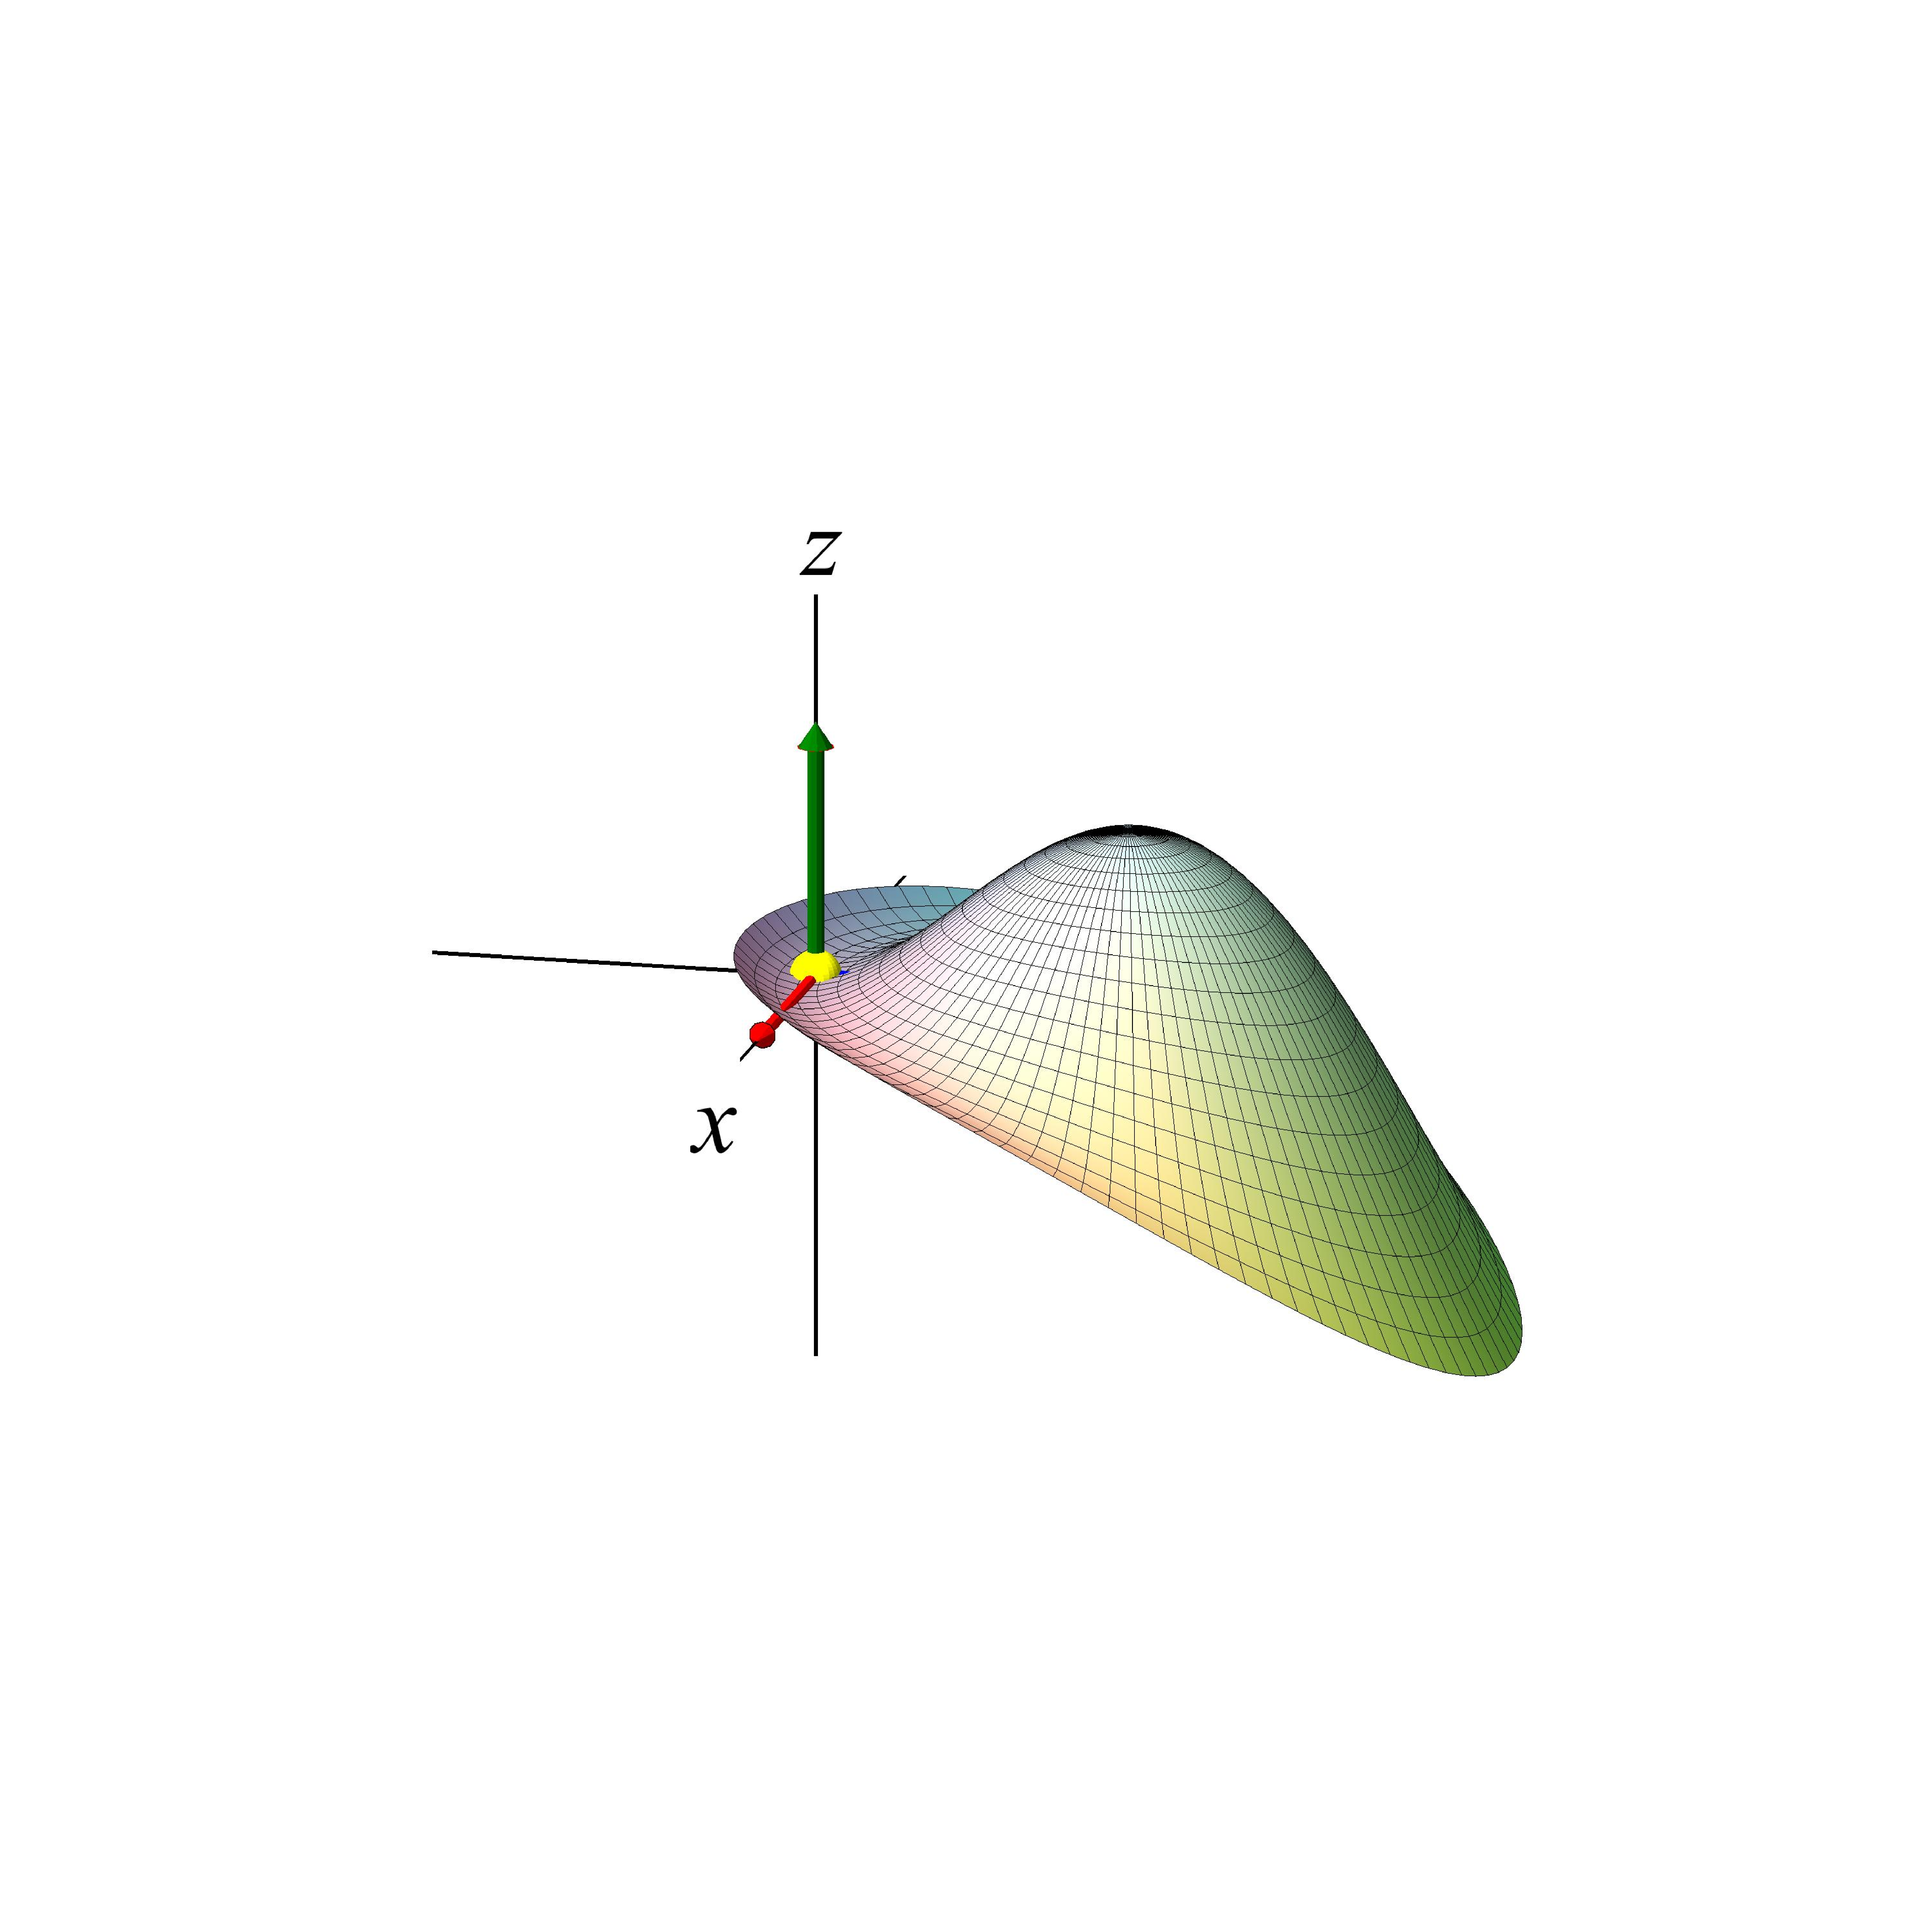
\includegraphics[height=55mm]{plotVar2Fig8.pdf}  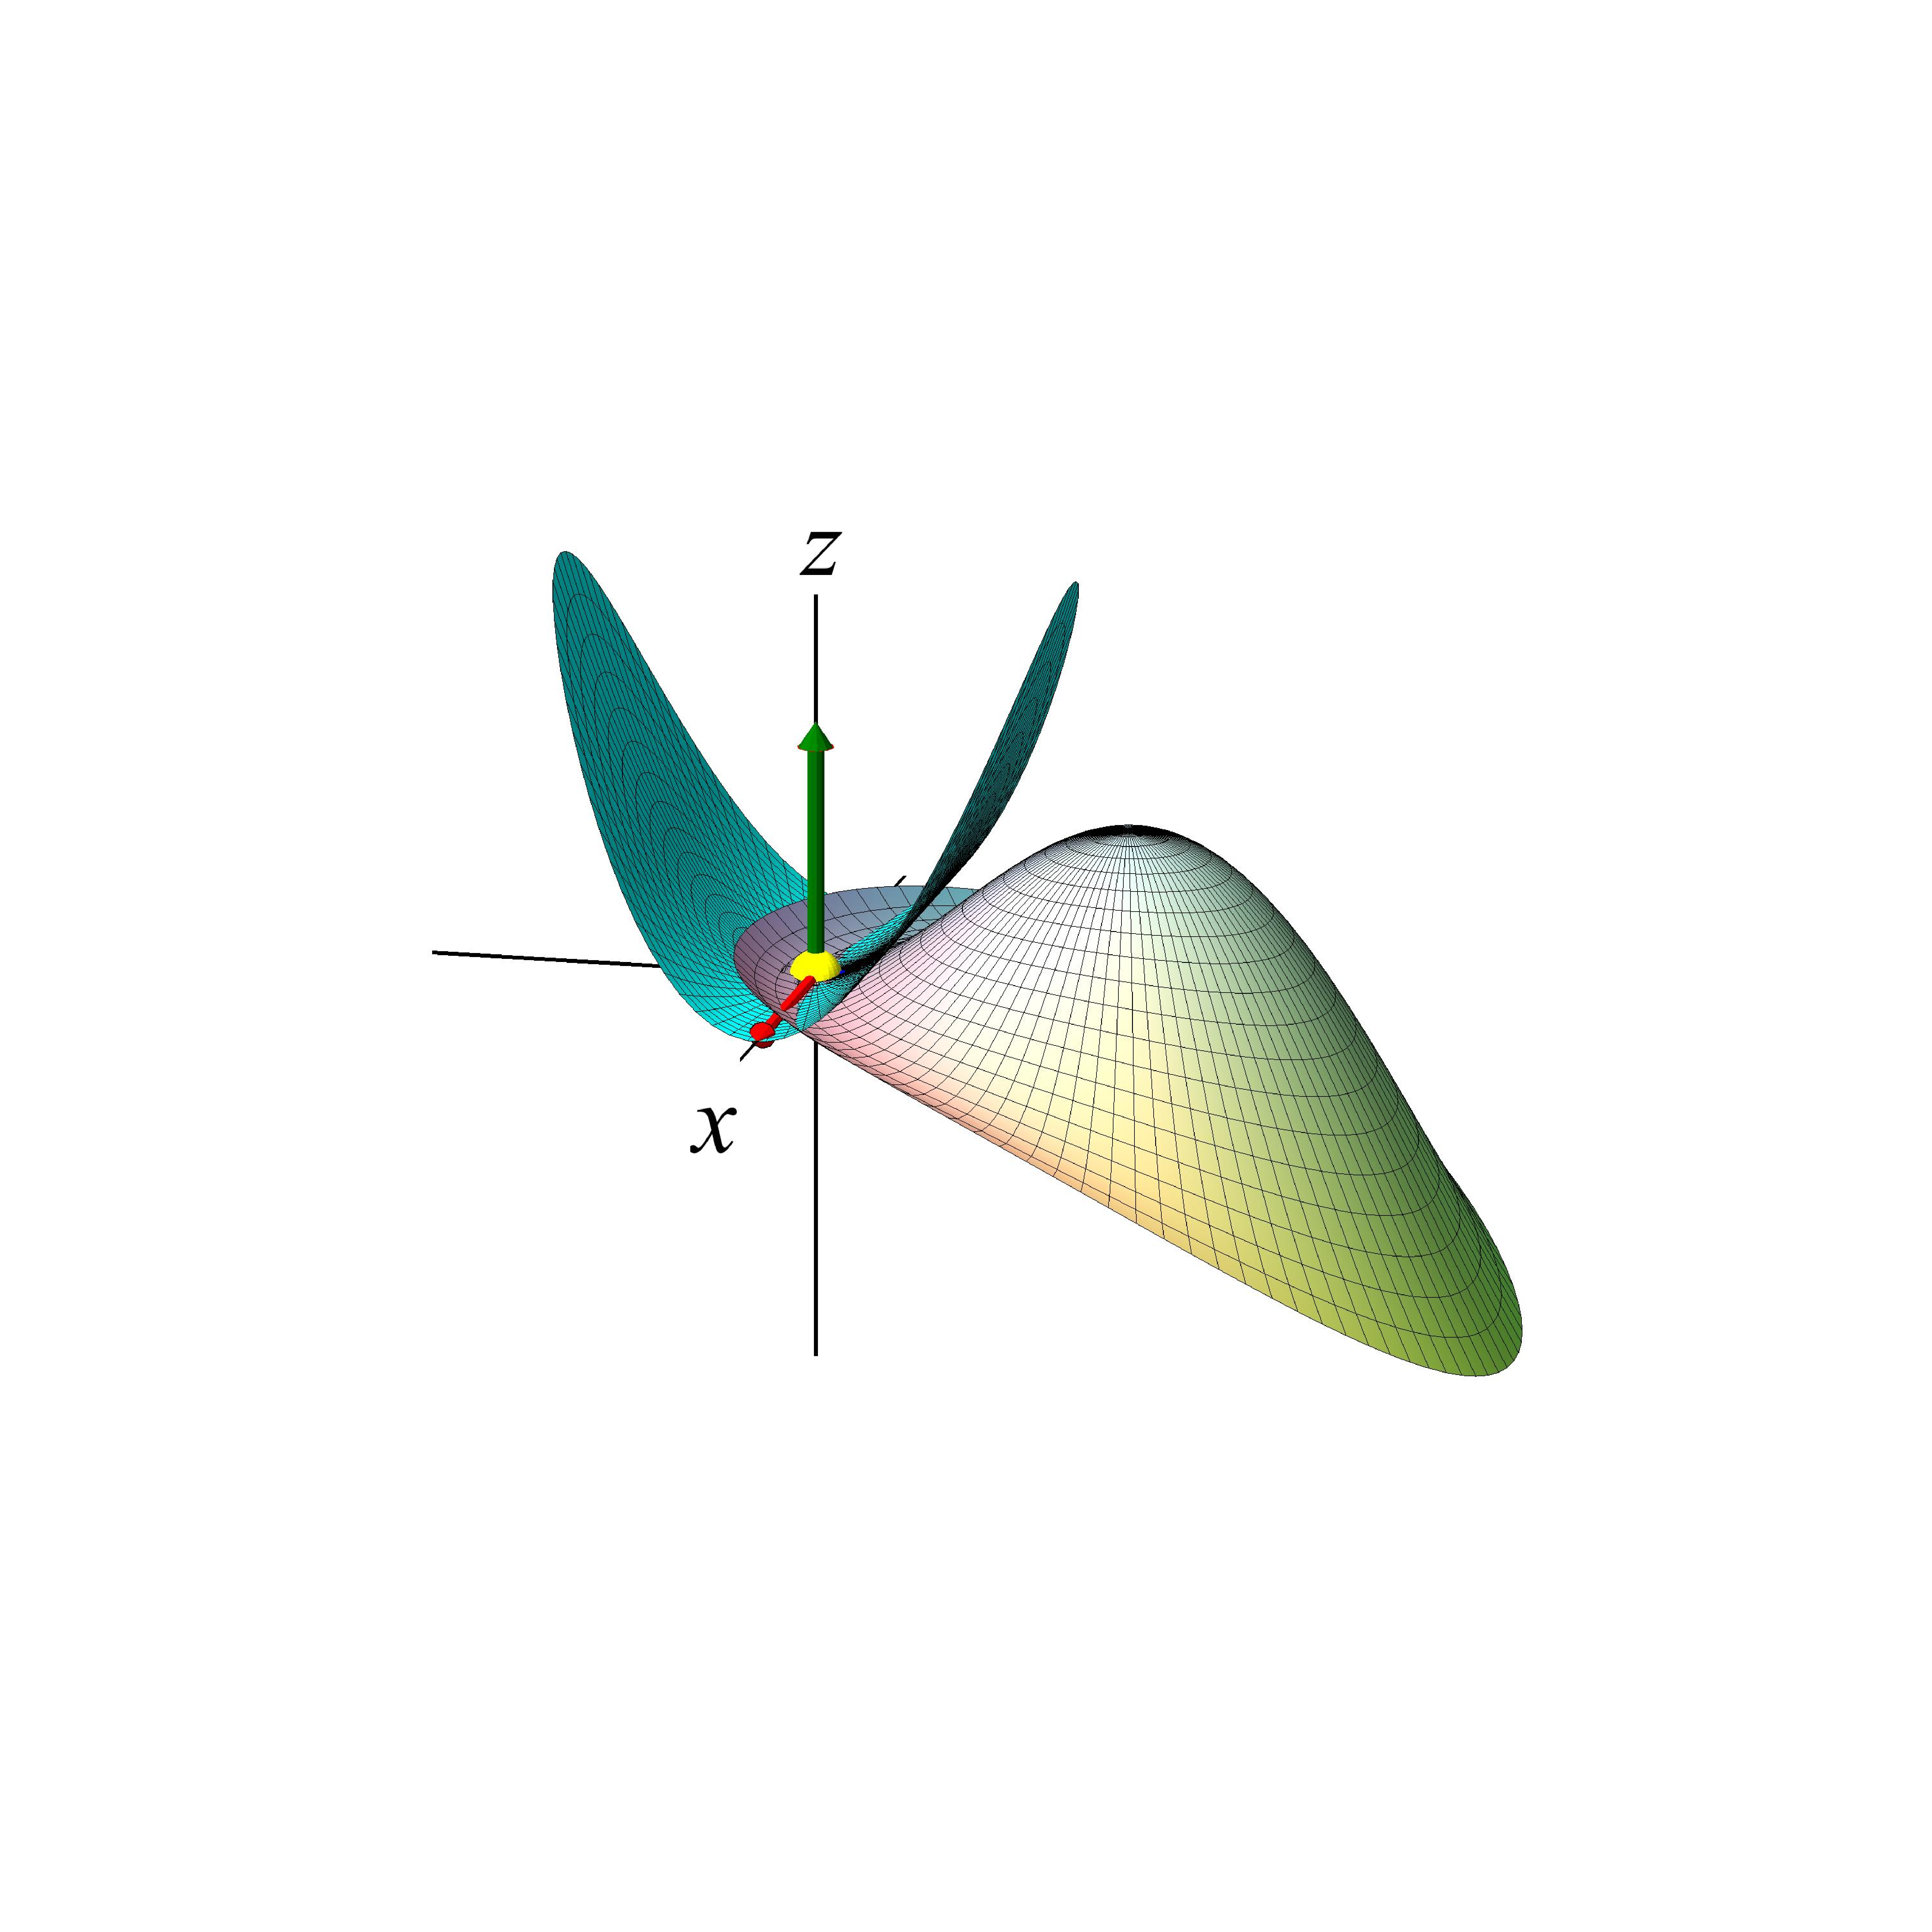
\includegraphics[height=55mm]{plotVar2FigApp8.pdf}  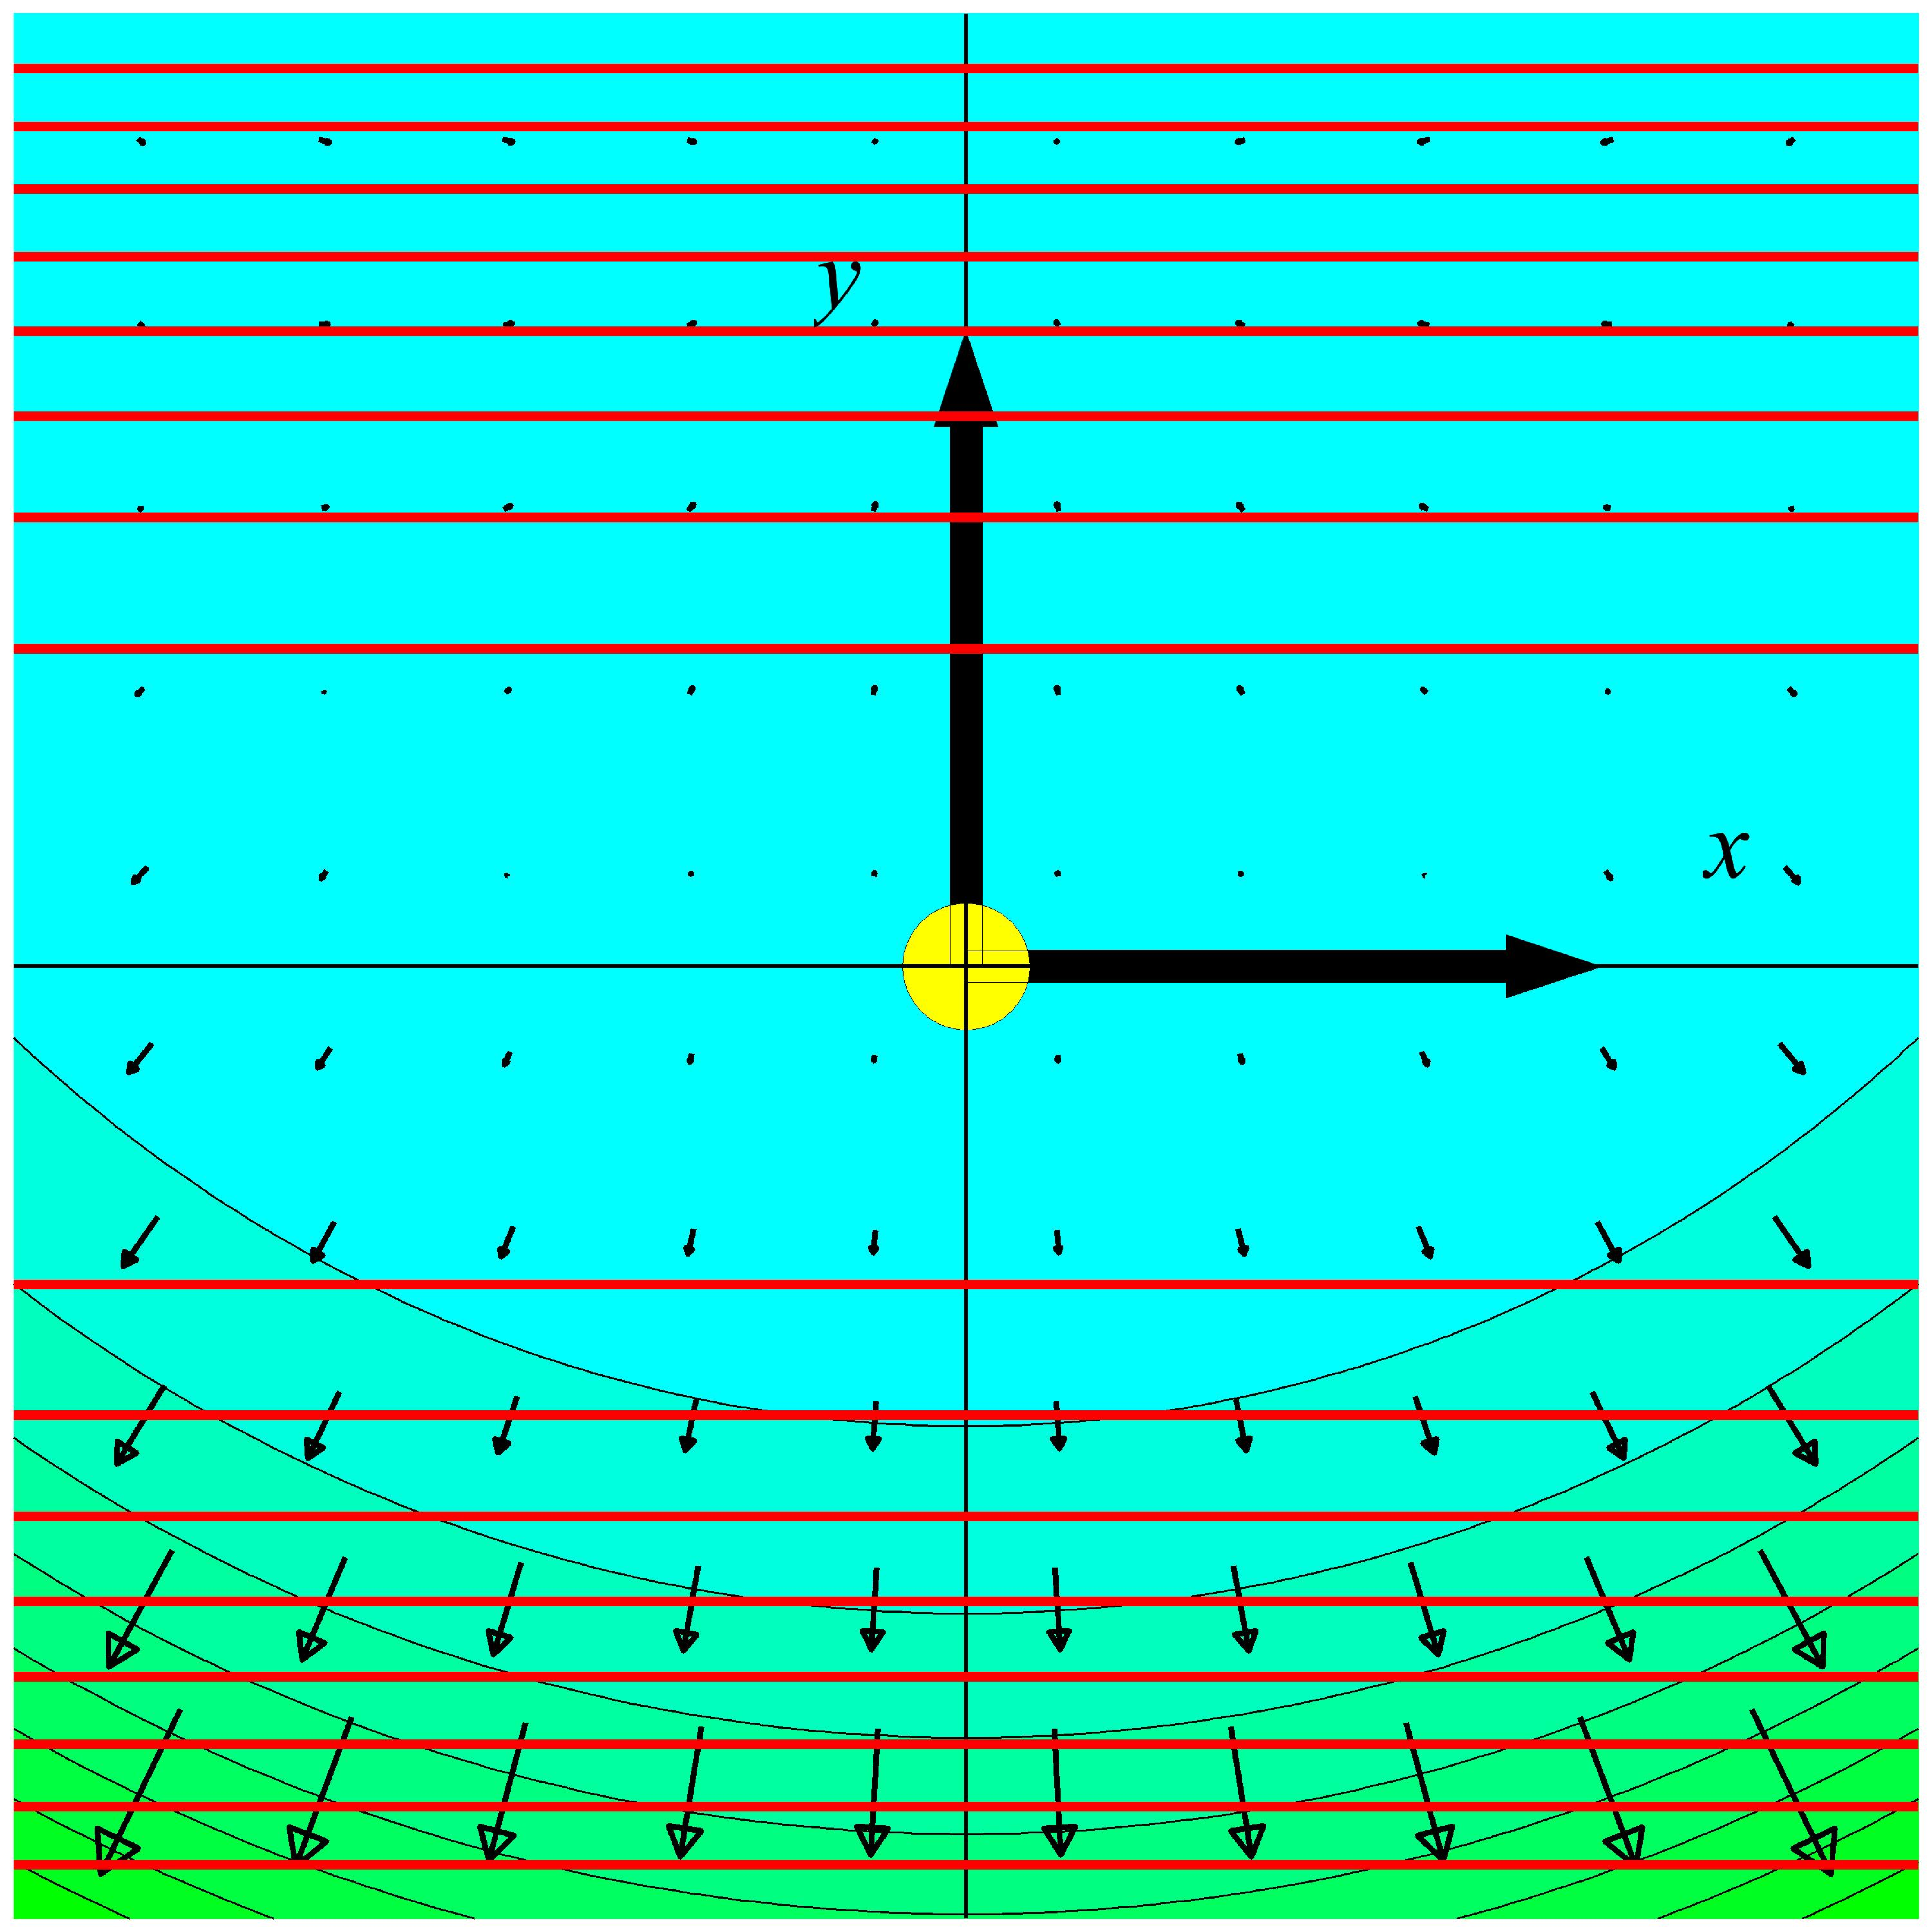
\includegraphics[height=55mm]{plotGrad8.pdf}}
\begin{center}
\caption{Til venstre: Grafen for funktionen $f(x,y) = \frac{1}{5}\cdot \left( 1 - (1-y)^{2} -x^{2}\right) \cdot \left( 4 - (2-y)^{2} - x^{2} \right)$. I midten: Grafen for $f(x,y)$ sammen med det approksimerende andengradspolynomium for funktionen med udviklingspunkt $(0, 0)$. Til højre: Gradientvektorfeltet for funktionen $f(x,y)$ og dens niveaukurver (sorte) samt niveaukurver for det approksimerende andengradspolynomium (røde) omkring det stationære punkt $(x_{0}, y_{0}) = (0, 0)$.} \label{figStatInspec4}
\end{center}
\end{figure}




\begin{aha}
Den funktion, der inspiceres i eksempel \ref{exampStatInspec4} har følgende forbavsende egenskab: Lad $\mathbf{r}(u)$ være parameterfremstillingen for en vilkårlig ret linje gennem $\mathbf{r}(0) = (0,0)$. Så har den sammensatte (højde-)funktion $h(u) = f(\mathbf{r}(u))$ et egentligt lokalt minimum i $u=0$. Dette forekommer altså til trods for, at funktionen $f(x,y)$ ikke selv har noget lokalt minimum i $(0,0)$. En fyldestgørende funktionsundersøgelse af en funktion af to variable omkring et stationært punkt kan altså ikke opnås ved blot at undersøge restriktionerne af funktionen til de rette  linjer igennem punktet!
\end{aha}



%%%%%%%%%%%%%%%%%%%%%%%%%%%%%%%%%%%%%%%%%%%%%%%%%%%
%%%%%%%%%%%%%%%%%%%%%%%%%%%%%%%%%%%%%%%%%%%%%%%%%%%
%%%%%%%%%%%%%%%%%%%%%%%%%%%%%%%%%%%%%%%%%%%%%%%%%%%



\begin{summary}
Denne eNote handler om analyse af funktioner af to variable.
\begin{itemize}
\item Vi bruger den kompakte notation for gradientvektorfeltet og Hesse-matricen som er givet ved
de afledede af $f(x,y)$ til og med anden orden:
\begin{equation}
\bm{\nabla}f(x_{0}, y_{0}) = (f'_{x}(x_{0}, y_{0}), f'_{y}(x_{0}, y_{0})) \quad ,
\end{equation}
\begin{equation}
\mathbf{H}f(x_{0}, y_{0}) = \left[
                              \begin{array}{cc}
                                f''_{xx}(x_{0}, y_{0}) & f''_{xy}(x_{0}, y_{0}) \\
                                f''_{yx}(x_{0}, y_{0}) & f''_{yy}(x_{0}, y_{0}) \\
                              \end{array}
                            \right] \quad .
\end{equation}
\item Det approksimerende polynomium af anden grad for $f(x,y)$ er så givet ved:

\begin{equation}
\begin{aligned}
P_{2, (x_{0}, y_{0})}(x,y) &= f(x_{0}, y_{0}) + \bm{\nabla}f(x_{0}, y_{0}) \bm{\cdot} (x-x_{0}, y-y_{0}) \\
&+ \frac{1}{2}\cdot \left[
                                          \begin{array}{cc}
                                            x-x_{0} & y-y_{0} \\
                                          \end{array}
                                        \right] \cdot \bm{H}f(x_{0}, y_{0})\cdot \left[
                                                                                   \begin{array}{c}
                                                                                         x-x_{0}  \\
                                                                                         y-y_{0}  \\
                                                                                   \end{array}                                                                                \right] \quad .
\end{aligned}
\end{equation}
\item Taylor's grænseformel for funktioner af to variable kan dermed skrives
\begin{equation}
\begin{aligned}
f(x,y) &= f(x_{0}, y_{0}) + \bm{\nabla}f(x_{0}, y_{0}) \bm{\cdot} (x-x_{0}, y-y_{0}) \\
&\phantom{abcdefghij}+ \frac{1}{2}\cdot \left[
                                          \begin{array}{cc}
                                            x-x_{0} & y-y_{0} \\
                                          \end{array}
                                        \right] \cdot \bm{H}f(x_{0}, y_{0})\cdot \left[
                                                                                   \begin{array}{c}
                                                                                         x-x_{0}  \\
                                                                                         y-y_{0}  \\
                                                                                   \end{array}
                                                                                 \right]\\
&\phantom{abcdefghij}+\rho^{2}_{(x_{0}, y_{0})}(x,y)\cdot \varepsilon_{f}(x-x_{0}, y-y_{0}) \quad .
\end{aligned}
\end{equation}
\item Stationære punkter $(x_{0}, y_{0})$ for funktioner $f(x,y)$ af to variable er karakteriserede ved at $\bm{\nabla}f(x_{0}, y_{0}) = (0,0)$.
\item Egenværdierne for Hesse-matricen i et stationært punkt kan hjælpe med at afgøre, om punktet er et egentligt lokalt maksimum- eller minimum-punkt for en glat funktion $f(x,y)$. Hvis egenværdierne er positive, så er punktet et egentligt lokalt minimumpunkt. Hvis de begge er negative, så er punktet et egentligt lokalt maksimumpunkt. Hvis egenværdierne begge er forskellige fra $0$ og har modsatte fortegn, så er der hverken maksimum- eller minimum-punkt i det stationære punkt.
\end{itemize}
\end{summary}



%%%%%%%%%%%%%%%%%%%%%%%%%%%%%%%%%%%%%%%%%%%%%
%%%%%%%%%%%%%%%%%%%%%%%%%%%%%%%%%%%%%%%%%%%%%
%%% HER SKAL DU STOPPE MED AT SKRIVE %%%%%%%%
%%%%%%%%%%%%%%%%%%%%%%%%%%%%%%%%%%%%%%%%%%%%%
%%%%%%%%%%%%%%%%%%%%%%%%%%%%%%%%%%%%%%%%%%%%%


\end{document} 

%%%%%%%%%%%%%%%%%%%%%%%%%%%%%%%%%%%%%%%%%%%%%%%%%%%
%%%%%%%%%%%%%%%%%%%%%%%%%%%%%%%%%%%%%%%%%%%%%%%%%%% 